% ---------------------------------------------------------------------------
%                   LATEX TEMPLATE FOR MARL PhD THESIS
% ---------------------------------------------------------------------------

% Taemin Cho put together a nice LaTeX class, that Oriol Nieto modified.
% Eric Humphrey added all of this sweet content, and made it available to
% the rest of MARLities.

% Everything is based on Harish Bhanderi's PhD/MPhil template, then Uni Cambridge
% http://www-h.eng.cam.ac.uk/help/tpl/textprocessing/ThesisStyle/
% corrected and extended in 2007 by Jakob Suckale, then MPI-CBG PhD programme
% and made available through OpenWetWare.org - the free biology wiki

%: Style file for Latex NYU-MARL:
% This template package can be found in ./Latex/Classes/
% It aims to follow the official NYU-Steinhardt guidelines:
%       http://steinhardt.nyu.edu/doctoral/dissertation/formatting
\documentclass[oneside, 12pt, letterpaper]{Latex/Classes/NYUdissertation}

%: Macro file for Latex
% Macros help you summarise frequently repeated Latex commands.
% Here, they are placed in an external file /Latex/Macros/MacroFile1.tex
% An macro that you may use frequently is the figuremacro (see introduction.tex)
% This file contains macros that can be called up from connected TeX files
% It helps to summarise repeated code, e.g. figure insertion (see below).

% insert a centered figure with caption and description
% parameters 1:filename, 2:title, 3:description and label
\newcommand{\figuremacro}[3]{
	\begin{figure}[htbp]
		\centering
		\includegraphics[width=1\textwidth]{#1}
		\caption[#2]{\textbf{#2} - #3}
		\label{#1}
	\end{figure}
}

% insert a centered figure with caption and description AND WIDTH
% parameters 1:filename, 2:title, 3:description and label, 4: textwidth
% textwidth 1 means as text, 0.5 means half the width of the text
\newcommand{\figuremacroW}[4]{
	\begin{figure}[htbp]
		\centering
		\includegraphics[width=#4\textwidth]{#1}
		\caption[#2]{\textbf{#2} - #3}
		\label{#1}
	\end{figure}
}

% inserts a figure with wrapped around text; only suitable for NARROW figs
% o is for outside on a double paged document; others: l, r, i(inside)
% text and figure will each be half of the document width
% note: long captions often crash with adjacent content; take care
% in general: above 2 macro produce more reliable layout
\newcommand{\figuremacroN}[3]{
	\begin{wrapfigure}{o}{0.5\textwidth}
		\centering
		\includegraphics[width=0.48\textwidth]{#1}
		\caption[#2]{{\small\textbf{#2} - #3}}
		\label{#1}
	\end{wrapfigure}
}

% predefined commands by Harish
\newcommand{\PdfPsText}[2]{
  \ifpdf
     #1
  \else
     #2
  \fi
}

\newcommand{\IncludeGraphicsH}[3]{
  \PdfPsText{\includegraphics[height=#2]{#1}}{\includegraphics[bb = #3, height=#2]{#1}}
}

\newcommand{\IncludeGraphicsW}[3]{
  \PdfPsText{\includegraphics[width=#2]{#1}}{\includegraphics[bb = #3, width=#2]{#1}}
}

\newcommand{\InsertFig}[3]{
  \begin{figure}[!htbp]
    \begin{center}
      \leavevmode
      #1
      \caption{#2}
      \label{#3}
    \end{center}
  \end{figure}
}


%%% Local Variables: 
%%% mode: latex
%%% TeX-master: "~/Documents/LaTeX/CUEDThesisPSnPDF/thesis"
%%% End: 


%: ----------------------------------------------------------------------
%:                  TITLE PAGE: name, degree,..
% ----------------------------------------------------------------------
% below is to generate the title page with crest and author name

%if output to PDF then put the following in PDF header
\ifpdf
    \pdfinfo { /Title  (An Exploration of Deep Learning in Content-Based Music Informatics)
               /Creator (TeX)
               /Producer (pdfTeX)
               /Author (Eric J. Humphrey ejhumphrey@nyu.edu)
               % /CreationDate (D:YYYYMMDDhhmmss)  %format D:YYYYMMDDhhmmss
               % /ModDate (D:YYYYMMDDhhmm)
               /Subject (Music Technology)
               /Keywords (Deep Learning, Digital Signal Processing, Music Informatics) }
         \pdfcatalog { /PageMode (/UseOutlines)
                  /OpenAction (fitbh)  }
\fi

\title{\doublespacing An Exploration of Deep Learning in Content-Based Music Informatics}

\threecommittee
{Professor Juan P. Bello, Chairperson}
{Professor Yann LeCun}
{Professor Panayotis Mavromatis}

\degree{Doctor of Philosophy}
\degreedate{2015}

% ----------------------------------------------------------------------
% The section below defines www links/email for author and institutions
% They will appear on the title page of the PDF and can be clicked

%: ----------------------- HELP: www links
% You can also see below how, www links are placed
% \href{http://www.something.net}{link text}

\author{\href{mailto:ejhumphrey@nyu.edu}{Eric J. Humphrey}}
\program{Program in \href{http://steinhardt.nyu.edu/music/technology/}{Music Technology}}
\department{Department of \href{http://steinhardt.nyu.edu/music/}{Music and Performing Arts Professions}}
\university{\href{http://www.nyu.edu/}{New York University}}
\crest{}%\includegraphics[width=3in]{NYUlogoLarge2597}}
\submittedtext{Submitted in partial fulfillment\\
  of the requirements for the degree of\\
  Doctor of Philosophy in the\\
  \href{http://steinhardt.nyu.edu/}{Steinhardt School of Culture, Education, and Human Development}}


% ----------------------------------------------------------------------

% turn of those nasty overfull and underfull hboxes
\hbadness=10000
\hfuzz=50pt
\makeindex

%:--------------------------------------------------------------
%:                  FRONT MATTER: dedications, abstract,..
% --------------------------------------------------------------

\begin{document}

%\hyphenpenalty=9000
%\frontmatter
\widowpenalty=10000
\clubpenalty=10000


%: ----------------------- generate cover page ------------------------
%\setstretch{1.2}
\maketitle  % command to print the title page with above variables
\makecopyright

%: ----------------------- abstract ------------------------

% Your institution may have specific regulations if you need an abstract and where it is to be placed in the document. The default here is just after title.

% 
% ----------------------------------------------------------------------
%                   LATEX TEMPLATE FOR PhD THESIS
% ----------------------------------------------------------------------

%: Style file for Latex
% Most style definitions are in the external file NYUdissertation
% In this template package, it can be found in ./Latex/Classes/

\documentclass[oneside, 12pt, letterpaper, nyustyle]{Latex/Classes/NYUdissertation}
%\documentclass[oneside, 12pt, letterpaper]{Latex/Classes/NYUdissertation}

%: Macro file for Latex
% Macros help you summarise frequently repeated Latex commands.
% Here, they are placed in an external file /Latex/Macros/MacroFile1.tex
% An macro that you may use frequently is the figuremacro (see introduction.tex)
% This file contains macros that can be called up from connected TeX files
% It helps to summarise repeated code, e.g. figure insertion (see below).

% insert a centered figure with caption and description
% parameters 1:filename, 2:title, 3:description and label
\newcommand{\figuremacro}[3]{
	\begin{figure}[htbp]
		\centering
		\includegraphics[width=1\textwidth]{#1}
		\caption[#2]{\textbf{#2} - #3}
		\label{#1}
	\end{figure}
}

% insert a centered figure with caption and description AND WIDTH
% parameters 1:filename, 2:title, 3:description and label, 4: textwidth
% textwidth 1 means as text, 0.5 means half the width of the text
\newcommand{\figuremacroW}[4]{
	\begin{figure}[htbp]
		\centering
		\includegraphics[width=#4\textwidth]{#1}
		\caption[#2]{\textbf{#2} - #3}
		\label{#1}
	\end{figure}
}

% inserts a figure with wrapped around text; only suitable for NARROW figs
% o is for outside on a double paged document; others: l, r, i(inside)
% text and figure will each be half of the document width
% note: long captions often crash with adjacent content; take care
% in general: above 2 macro produce more reliable layout
\newcommand{\figuremacroN}[3]{
	\begin{wrapfigure}{o}{0.5\textwidth}
		\centering
		\includegraphics[width=0.48\textwidth]{#1}
		\caption[#2]{{\small\textbf{#2} - #3}}
		\label{#1}
	\end{wrapfigure}
}

% predefined commands by Harish
\newcommand{\PdfPsText}[2]{
  \ifpdf
     #1
  \else
     #2
  \fi
}

\newcommand{\IncludeGraphicsH}[3]{
  \PdfPsText{\includegraphics[height=#2]{#1}}{\includegraphics[bb = #3, height=#2]{#1}}
}

\newcommand{\IncludeGraphicsW}[3]{
  \PdfPsText{\includegraphics[width=#2]{#1}}{\includegraphics[bb = #3, width=#2]{#1}}
}

\newcommand{\InsertFig}[3]{
  \begin{figure}[!htbp]
    \begin{center}
      \leavevmode
      #1
      \caption{#2}
      \label{#3}
    \end{center}
  \end{figure}
}


%%% Local Variables: 
%%% mode: latex
%%% TeX-master: "~/Documents/LaTeX/CUEDThesisPSnPDF/thesis"
%%% End: 


%: ----------------------------------------------------------------------
%:                  TITLE PAGE: name, degree,..
% ----------------------------------------------------------------------
% below is to generate the title page with crest and author name

%if output to PDF then put the following in PDF header
\ifpdf
    \pdfinfo { /Title  (Bear Claw Macaroon Tiramisu Cheesecake)
               /Creator (TeX)
               /Producer (pdfTeX)
               /Author (Your Name addy@nyu.edu)
               /Subject (Music Technology)
               /Keywords (Marzipan, jujubes, pudding, sesame snaps) }
         \pdfcatalog { /PageMode (/UseOutlines)
                  /OpenAction (fitbh)  }
\fi

\abstracttitle{\doublespacing Bear Claw Macaroon Tiramisu Cheesecake}

\threecommittee
{Professor I.~M. Smart, Chairperson}
{Professor Beardsley Wordsworth}
{Professor Norma Hazelwood}

\degree{Doctor of Philosophy}
\degreedate{2014}


% ----------------------------------------------------------------------
% The section below defines www links/email for author and institutions
% They will appear on the title page of the PDF and can be clicked

%: ----------------------- HELP: www links
% You can also see below how, www links are placed
% \href{http://www.something.net}{link text}

\author{\href{mailto:addy@nyu.edu}{Your Name}}
\program{Program in \href{http://steinhardt.nyu.edu/music/technology/}{Music Technology}}
\department{Department of \href{http://steinhardt.nyu.edu/music/}{Music and Performing Arts Professions}}
\university{\href{http://www.nyu.edu/}{New York University}}
\crest{\includegraphics[width=3in]{NYUlogoLarge2597}}
\submittedtext{Submitted in partial fulfillment\\
  of the requirements for the degree of\\
  Doctor of Philosophy in the\\
  \href{http://steinhardt.nyu.edu/}{Steinhardt School of Culture, Education, and Human Development}}

% ----------------------------------------------------------------------

% turn of those nasty overfull and underfull hboxes
\hbadness=10000
\hfuzz=50pt
\makeindex

\begin{document}

\frontmatter
%: ----------------------- generate cover page ------------------------
\setstretch{1.2}
\maketitle  % command to print the title page with above variables
%
% ----------------------------------------------------------------------
%                   LATEX TEMPLATE FOR PhD THESIS
% ----------------------------------------------------------------------

%: Style file for Latex
% Most style definitions are in the external file NYUdissertation
% In this template package, it can be found in ./Latex/Classes/

\documentclass[oneside, 12pt, letterpaper, nyustyle]{Latex/Classes/NYUdissertation}
%\documentclass[oneside, 12pt, letterpaper]{Latex/Classes/NYUdissertation}

%: Macro file for Latex
% Macros help you summarise frequently repeated Latex commands.
% Here, they are placed in an external file /Latex/Macros/MacroFile1.tex
% An macro that you may use frequently is the figuremacro (see introduction.tex)
% This file contains macros that can be called up from connected TeX files
% It helps to summarise repeated code, e.g. figure insertion (see below).

% insert a centered figure with caption and description
% parameters 1:filename, 2:title, 3:description and label
\newcommand{\figuremacro}[3]{
	\begin{figure}[htbp]
		\centering
		\includegraphics[width=1\textwidth]{#1}
		\caption[#2]{\textbf{#2} - #3}
		\label{#1}
	\end{figure}
}

% insert a centered figure with caption and description AND WIDTH
% parameters 1:filename, 2:title, 3:description and label, 4: textwidth
% textwidth 1 means as text, 0.5 means half the width of the text
\newcommand{\figuremacroW}[4]{
	\begin{figure}[htbp]
		\centering
		\includegraphics[width=#4\textwidth]{#1}
		\caption[#2]{\textbf{#2} - #3}
		\label{#1}
	\end{figure}
}

% inserts a figure with wrapped around text; only suitable for NARROW figs
% o is for outside on a double paged document; others: l, r, i(inside)
% text and figure will each be half of the document width
% note: long captions often crash with adjacent content; take care
% in general: above 2 macro produce more reliable layout
\newcommand{\figuremacroN}[3]{
	\begin{wrapfigure}{o}{0.5\textwidth}
		\centering
		\includegraphics[width=0.48\textwidth]{#1}
		\caption[#2]{{\small\textbf{#2} - #3}}
		\label{#1}
	\end{wrapfigure}
}

% predefined commands by Harish
\newcommand{\PdfPsText}[2]{
  \ifpdf
     #1
  \else
     #2
  \fi
}

\newcommand{\IncludeGraphicsH}[3]{
  \PdfPsText{\includegraphics[height=#2]{#1}}{\includegraphics[bb = #3, height=#2]{#1}}
}

\newcommand{\IncludeGraphicsW}[3]{
  \PdfPsText{\includegraphics[width=#2]{#1}}{\includegraphics[bb = #3, width=#2]{#1}}
}

\newcommand{\InsertFig}[3]{
  \begin{figure}[!htbp]
    \begin{center}
      \leavevmode
      #1
      \caption{#2}
      \label{#3}
    \end{center}
  \end{figure}
}


%%% Local Variables: 
%%% mode: latex
%%% TeX-master: "~/Documents/LaTeX/CUEDThesisPSnPDF/thesis"
%%% End: 


%: ----------------------------------------------------------------------
%:                  TITLE PAGE: name, degree,..
% ----------------------------------------------------------------------
% below is to generate the title page with crest and author name

%if output to PDF then put the following in PDF header
\ifpdf
    \pdfinfo { /Title  (Bear Claw Macaroon Tiramisu Cheesecake)
               /Creator (TeX)
               /Producer (pdfTeX)
               /Author (Your Name addy@nyu.edu)
               /Subject (Music Technology)
               /Keywords (Marzipan, jujubes, pudding, sesame snaps) }
         \pdfcatalog { /PageMode (/UseOutlines)
                  /OpenAction (fitbh)  }
\fi

\abstracttitle{\doublespacing Bear Claw Macaroon Tiramisu Cheesecake}

\threecommittee
{Professor I.~M. Smart, Chairperson}
{Professor Beardsley Wordsworth}
{Professor Norma Hazelwood}

\degree{Doctor of Philosophy}
\degreedate{2014}


% ----------------------------------------------------------------------
% The section below defines www links/email for author and institutions
% They will appear on the title page of the PDF and can be clicked

%: ----------------------- HELP: www links
% You can also see below how, www links are placed
% \href{http://www.something.net}{link text}

\author{\href{mailto:addy@nyu.edu}{Your Name}}
\program{Program in \href{http://steinhardt.nyu.edu/music/technology/}{Music Technology}}
\department{Department of \href{http://steinhardt.nyu.edu/music/}{Music and Performing Arts Professions}}
\university{\href{http://www.nyu.edu/}{New York University}}
\crest{\includegraphics[width=3in]{NYUlogoLarge2597}}
\submittedtext{Submitted in partial fulfillment\\
  of the requirements for the degree of\\
  Doctor of Philosophy in the\\
  \href{http://steinhardt.nyu.edu/}{Steinhardt School of Culture, Education, and Human Development}}

% ----------------------------------------------------------------------

% turn of those nasty overfull and underfull hboxes
\hbadness=10000
\hfuzz=50pt
\makeindex

\begin{document}

\frontmatter
%: ----------------------- generate cover page ------------------------
\setstretch{1.2}
\maketitle  % command to print the title page with above variables
%
% ----------------------------------------------------------------------
%                   LATEX TEMPLATE FOR PhD THESIS
% ----------------------------------------------------------------------

%: Style file for Latex
% Most style definitions are in the external file NYUdissertation
% In this template package, it can be found in ./Latex/Classes/

\documentclass[oneside, 12pt, letterpaper, nyustyle]{Latex/Classes/NYUdissertation}
%\documentclass[oneside, 12pt, letterpaper]{Latex/Classes/NYUdissertation}

%: Macro file for Latex
% Macros help you summarise frequently repeated Latex commands.
% Here, they are placed in an external file /Latex/Macros/MacroFile1.tex
% An macro that you may use frequently is the figuremacro (see introduction.tex)
\include{Latex/Macros/MacroFile1}

%: ----------------------------------------------------------------------
%:                  TITLE PAGE: name, degree,..
% ----------------------------------------------------------------------
% below is to generate the title page with crest and author name

%if output to PDF then put the following in PDF header
\ifpdf
    \pdfinfo { /Title  (Bear Claw Macaroon Tiramisu Cheesecake)
               /Creator (TeX)
               /Producer (pdfTeX)
               /Author (Your Name addy@nyu.edu)
               /Subject (Music Technology)
               /Keywords (Marzipan, jujubes, pudding, sesame snaps) }
         \pdfcatalog { /PageMode (/UseOutlines)
                  /OpenAction (fitbh)  }
\fi

\abstracttitle{\doublespacing Bear Claw Macaroon Tiramisu Cheesecake}

\threecommittee
{Professor I.~M. Smart, Chairperson}
{Professor Beardsley Wordsworth}
{Professor Norma Hazelwood}

\degree{Doctor of Philosophy}
\degreedate{2014}


% ----------------------------------------------------------------------
% The section below defines www links/email for author and institutions
% They will appear on the title page of the PDF and can be clicked

%: ----------------------- HELP: www links
% You can also see below how, www links are placed
% \href{http://www.something.net}{link text}

\author{\href{mailto:addy@nyu.edu}{Your Name}}
\program{Program in \href{http://steinhardt.nyu.edu/music/technology/}{Music Technology}}
\department{Department of \href{http://steinhardt.nyu.edu/music/}{Music and Performing Arts Professions}}
\university{\href{http://www.nyu.edu/}{New York University}}
\crest{\includegraphics[width=3in]{NYUlogoLarge2597}}
\submittedtext{Submitted in partial fulfillment\\
  of the requirements for the degree of\\
  Doctor of Philosophy in the\\
  \href{http://steinhardt.nyu.edu/}{Steinhardt School of Culture, Education, and Human Development}}

% ----------------------------------------------------------------------

% turn of those nasty overfull and underfull hboxes
\hbadness=10000
\hfuzz=50pt
\makeindex

\begin{document}

\frontmatter
%: ----------------------- generate cover page ------------------------
\setstretch{1.2}
\maketitle  % command to print the title page with above variables
%\include{frontmatter/abstract}
\begin{abstract}
\null\vspace{0.4in}
\doublespacing

This template provides the basic skeleton necessary to complete your dissertation.
It has been populated with cupcake ipsum in the hopes that this sweet gibberish will make the task less daunting.
Compiling this document is mostly straightforward in TexShop, but the glossary must be compiled manually; your mileage may vary in other environments.
Additionally, it is strongly recommended that you use a version control system, e.g. git, while writing your dissertation. 
If you do so, you may find it significantly easier to keep each sentence on its own line, which plays to the atomicity of ongoing modifications.

\end{abstract}

\clearpage
\thispagestyle{empty}
\doublespacing
\null\vfill
I hereby guarantee that no part of the dissertation which I have submitted for publication has been heretofore published and/or copyrighted in the United States of America, except in the case of passages quoted from other published sources; that I am the sole author and proprietor of said dissertation; that the dissertation contains no matter which, if published, will be libelous or otherwise injurious, or infringe in any way the copyright of any other party; and that I will defend, indemnify and hold harmless New York University against all suits and proceedings which may be brought and against all claims which may be made against New York University by reason of the publication of said dissertation.
\vfill
\hfill\begin{tabular}{@{}ll@{}}
\makebox[2.5in]{\hrulefill} & \makebox[2in]{\hrulefill}\\[-2em]
\textit{Signature} & \textit{Date}
\end{tabular}
\null\vfill
\end{document}

\begin{abstract}
\null\vspace{0.4in}
\doublespacing

This template provides the basic skeleton necessary to complete your dissertation.
It has been populated with cupcake ipsum in the hopes that this sweet gibberish will make the task less daunting.
Compiling this document is mostly straightforward in TexShop, but the glossary must be compiled manually; your mileage may vary in other environments.
Additionally, it is strongly recommended that you use a version control system, e.g. git, while writing your dissertation. 
If you do so, you may find it significantly easier to keep each sentence on its own line, which plays to the atomicity of ongoing modifications.

\end{abstract}

\clearpage
\thispagestyle{empty}
\doublespacing
\null\vfill
I hereby guarantee that no part of the dissertation which I have submitted for publication has been heretofore published and/or copyrighted in the United States of America, except in the case of passages quoted from other published sources; that I am the sole author and proprietor of said dissertation; that the dissertation contains no matter which, if published, will be libelous or otherwise injurious, or infringe in any way the copyright of any other party; and that I will defend, indemnify and hold harmless New York University against all suits and proceedings which may be brought and against all claims which may be made against New York University by reason of the publication of said dissertation.
\vfill
\hfill\begin{tabular}{@{}ll@{}}
\makebox[2.5in]{\hrulefill} & \makebox[2in]{\hrulefill}\\[-2em]
\textit{Signature} & \textit{Date}
\end{tabular}
\null\vfill
\end{document}

\begin{abstract}
\null\vspace{0.4in}
\doublespacing

This template provides the basic skeleton necessary to complete your dissertation.
It has been populated with cupcake ipsum in the hopes that this sweet gibberish will make the task less daunting.
Compiling this document is mostly straightforward in TexShop, but the glossary must be compiled manually; your mileage may vary in other environments.
Additionally, it is strongly recommended that you use a version control system, e.g. git, while writing your dissertation. 
If you do so, you may find it significantly easier to keep each sentence on its own line, which plays to the atomicity of ongoing modifications.

\end{abstract}

\clearpage
\thispagestyle{empty}
\doublespacing
\null\vfill
I hereby guarantee that no part of the dissertation which I have submitted for publication has been heretofore published and/or copyrighted in the United States of America, except in the case of passages quoted from other published sources; that I am the sole author and proprietor of said dissertation; that the dissertation contains no matter which, if published, will be libelous or otherwise injurious, or infringe in any way the copyright of any other party; and that I will defend, indemnify and hold harmless New York University against all suits and proceedings which may be brought and against all claims which may be made against New York University by reason of the publication of said dissertation.
\vfill
\hfill\begin{tabular}{@{}ll@{}}
\makebox[2.5in]{\hrulefill} & \makebox[2in]{\hrulefill}\\[-2em]
\textit{Signature} & \textit{Date}
\end{tabular}
\null\vfill
\end{document}


%: ----------------------- tie in front matter ------------------------
\doublespacing

\chapter*{Acknowledgements}

There once was a time I thought it was some happy accident that I kept finding myself in exactly the right place.
Be it college, career, or concert, it always felt like gravity, quietly inevitable, pulling me into the things I should do, the places I should go, the opportunities I should pursue.
But now, on the backside of this arc, I can see quite plainly that I always had the direction wrong; it was never a pull, but a push.
Come to think of it, for as long as I can seem to recall, I have been lucky enough to be surrounded by those who would inspire, encourage, force, drag, and challenge me to always be better.
I am nothing short of blessed to be graced by the company and influence of such wonderful human beings, and will try my best to thank as many of you as I can here.

First and foremost, I am forever grateful to my grandparents ---Glendolyn \& Norman, Elizabeth \& Frank--- for their myriad contributions, both concrete and intangible.
It is only for their love, diligence and sacrifice that any of this is possible (but what I wouldn't give to see your reactions now).
This goes doubly so for my parents, Sharon \& Branden, who took a computer-tinkering, dinosaur-building, saxophone-wielding dreamer and turned him into a computer-sciencing, wood-working, guitar-wielding dreamer.
Good job, guys.
An extra special thanks goes to my brothers, Steve \& Tim, for all adventures, past, present, and future.

% Formative years
To those who had a most profound impact on my younger self:
Paul Andersen, who helped introduce me to music, and more importantly, improvisation;
Mary Bolton, who truly was ``Mary E. Best'', and is near entirely to thank (or blame) for my egregious use of analogy;
Matt McGuire, who instilled the virtues of hard work, effort, and discipline, and earned my deepest respect for it;
and Jayant Datta, who saw something in a kid with long hair and an unhealthy love of delay pedals, and happily pushed him down the rabbit hole of higher education.

Corey and Colby,
Chris Stef and Glen
Patrick and Reid

Ron, Aron, Areti, Jon, Taemin
Uri, Braxton
Finn, Michael, Rachel, Andrew
Brian and Justin
Ryan Rifkin

Committee
Panos,
Yann,
Juan



%: ----------------------- contents ------------------------
% levels are: 0 - chapter, 1 - section, 2 - subsection, 3 - subsubsection
\setcounter{secnumdepth}{3} % organisational level that receives a numbers (NYU Steinhardt recommends level 0, which is pretty hideous)
\setcounter{tocdepth}{2}    % print table of contents for level 2
\singlespacing
\tableofcontents            % print the table of contents
%\addcontentsline{toc}{section}{continued}
%: ----------------------- list of figures/tables ------------------------
\clearpage
\listoftables                   % print list of tables
\clearpage
\listoffigures                  % print list of figures

%: ----------------------- glossary ------------------------

% Tie in external source file for definitions: /frontmatter/glossary.tex
% Glossar entries can also be defined in the main text. See glossary.tex

% this file is called up by thesis.tex
% content in this file will be fed into the main document

\newacronym{tcap}{TCAP}{Toffee chocolate apple pie}


\newglossaryentry{Chupa chups}
{
  name={chupa chups},
  description= {Powder fruitcake ice cream ice cream brownie biscuit ice cream ice cream}
}

%\makeglossaries
\clearpage
\printglossaries


\chapterbegin

%: ----------------------- epigraph ------------------------

\chapter*{}

\begin{quote}

``What's it matter? Does it matter, \\
If we're all matter when we're done, \\
When the sky is full of zeros and ones?''

\end{quote}

\vspace{1in}
\hspace{2in}
-Andrew Bird, {\it Masterfade}


%: --------------------------------------------------------------
%:                  MAIN DOCUMENT SECTION
% --------------------------------------------------------------

% the main text starts here with the introduction, 1st chapter,...

\mainmatter
\doublespacing
%: ----------------------- subdocuments ------------------------

% Parts of the thesis are included below. Rename the files as required.
% But take care that the paths match. You can also change the order of appearance by moving the include commands.


% this file is called up by thesis.tex
% content in this file will be fed into the main document

%: ----------------------- introduction file header -----------------------
% the code below specifies where the figures are stored
\graphicspath{{1/figures/}}

\chapter{Introduction}
\label{chp:introduction}

% Information age
It goes without saying that we live in the Age of Information, our day to day experiences awash in a flood of data.
As a society, we buy, sell, consume and produce information in unprecedented quantities.
% More data than anyone can handle
Given the accelerating rate at which information is created, one of the fundamental challenges facing the modern world is simply making sense of all this data.
% Google bitches
The quintessential response to this obstacle is embodied by Google, whose collective \emph{raison d'\^etre} is the organization and indexing of the world's information.
To appreciate the value and reach of this technology, one only needs to imagine how impossible it would be to browse the Internet without a search engine.

 % is a significant research effort behind the development of computational methods and algorithms to help make information universally accessible and useful. %, and this is particularly evident in the realm of music.

% Information overload, yo

% This domain is broadly referred to as \emph{information retrieval} (IR), and has grown rapidly in recent years, with various subdomains coalescing around application-specific topics.

Understandably, a variety of specialized disciplines have formed under the auspices of developing systems to help humans navigate and understand massive amounts of information.
Coalescing around the turn of the century, music informatics is one such instance, drawing from several diverse fields, including electrical engineering, music psychology, computer science, machine learning, and music theory, among others.
Now encompassing a wide spectrum of application areas and the kinds of data considered---from audio signals and music blogs to album covers and online social interactions---music informatics can be broadly defined as the study of information related to, or is a result of, musical activity.

% IR Formulation
At a high level, tackling this problem of ``information overload'' in music is captured by a simple, general analogy: how exactly \emph{does} one find a needle in a haystack?
To answer this question, any system, computational or otherwise, must solve two related problems:
first, it is necessary to describe the intrinsic qualities of the item of interest, e.g. a needle is metal, sharp, thin, etc;
and second, it is necessary to evaluate the extrinsic relationships between items to determine relevance.
A piece of hay is certainly not a needle, for example, but is a pin close enough?
Along what criteria might we gauge similarity, or classify objects into groups?
Emphasizing the distinction, \emph{description} focuses on absolute representation, whereas \emph{comparison} is concerned with relative associations.

% Human provided descriptions and relationships
To date, the most successful approaches to large-scale information systems leverage human-provided signals to achieve rich content descriptions.
Building on top of robust representations simplifies the problem greatly, and good progress has been made toward the development of useful applications.
% Human signals about the content
For example, the Netflix Prize challenge\footnote{\url{http://www.netflixprize.com/}} ---a contest to find the best system for automatically predicting a user's enjoyment of a movie--- was built exclusively on movie ratings contributed by a large collection of other users.
% Links between content
Similarly, Google's \emph{PageRank} algorithm associates websites based on how users have linked different pages together, thus facilitating the process of traversing the Internet \cite{Page1999Pagerank}.

% Music is a different ballgame, y'all; document description is wicked hard.
While this strategy of leveraging manual content description has proven successful in large-scale music recommendation, such as Pandora Radio\footnote{\url{http://www.pandora.com/}}, its application to more general music information problems is fundamentally limited, manifesting in three related ways.
First, human-provided information commonly used in such systems ---clicks, likes, listens or shares--- are a naturally occurring by-product of music consumption.
It is one thing to obtain a ``thumbs up'' for a song; it is quite another to ask that same user to provide a chord transcription of it.
Second, manual music description may require a high degree of expertise or effort to perform.
The average music listener is not truly capable of transcribing chords from a sound recording, whether or not she possesses the time or willingness to attempt it.
Finally, even given the skill, motivation, and infrastructure to manually describe music, this approach cannot scale to \emph{all} music content, now or in the future.
The Music Genome Project\footnote{\url{https://www.pandora.com/about/mgp}}, for example, has resulted in the manual annotation of some 1M commercial recordings, at a pace of 20-30 minutes per track;
the iTunes Music Store, however, now offers over 43M tracks worldwide\footnote{According to \url{http://www.apple.com/itunes/music/}, accessed 20 April, 2015.}.
To illustrate how vast this discrepancy is, consider the following: even assuming the lower bound of 20 minutes, it would still take one poor individual \emph{1,600 years} of non-stop annotation to close that gap.
More importantly, this only considers commercial music recordings, neglecting amateur or user-generated content from websites like YouTube\footnote{https://www.youtube.com/} or Soundcloud\footnote{\url{https://soundcloud.com/}}, the addition of which makes this goal even more insurmountable.
Given the sheer impossibility for humans to meaningfully describe all recorded music, now and in the future, truly scalable music information systems will require good automatic systems to perform this task.

% Music description is good, state of the art is bad
Thus, the development of computational systems to describe music signals, a flavor of \emph{computer audition} referred to as content-based music informatics, is both a valuable and fascinating problem.
In addition to facilitating the search and retrieval of large music collections, automatic systems capable of expert-level music description are invaluable to users who are unable to perform the task themselves, e.g. music transcription.
Notably, this problem is also very much unsolved, and given an apparent deceleration of progress, some in the field of music informatics have begun to question the efficacy of traditional research methods.
% Statement of the issues?
Simultaneously, in the related fields of computer vision and automatic speech recognition, a branch of machine learning, referred to as \emph{deep learning}, has shown great performance in various domains, toppling many long-standing benchmarks.
On closer inspection, one recognizes considerable conceptual overlap between deep learning and conventional music signal processing systems, further encouraging this promising union.

% Research goal
Synthesizing these observations, this study explores deep learning as a general approach to the design of computer audition systems for music description applications.
More specifically, the proposed research method proceeds thusly:
first, methods and trends in content-based music informatics are reviewed in an effort to understand why progress in this domain may be decellerating, and, in doing so, identify possible deficiencies in this methodology;
standard approaches to music signal processing are then reformulated in the language and concepts of deep learning, and subsequently applied to classic music informatics problems;
finally, the behavior of these deep learning systems is deconstructed in order to illustrate the advantages and challenges inherent to this paradigm.


\section{Scope of this Study}
\label{sec:scope}

% Functionally model intelligent behavior
% how to judge whether or not the description is good? and what is good?
% hinges on how quality is defined
% assessment is driven by how the system behaves compared to

This study explores the use of deep learning in the development of systems for automatic music description.
Consistent with the larger body of machine perception research, the work presented here aims to computationally model the relationship between stimuli and observations made by an intelligent agent.
In this case, ``stimuli'' are digital signals representing acoustic waves, e.g. sound, ``observations'' are semantic descriptions in a particular namespace, e.g. timbre or harmony, and the agent being modeled is an intelligent human, e.g. an expert music listener.
In practice, the namespace of descriptions considered is constrained to a particular task or application, such as instrument recognition or chord estimation.

Furthermore, if the relationship between stimuli and observation is not a function of the agent, this mapping is said to be \emph{objective}.
Objective relationships are those that are true absolutely by definition, such as the statement ``A C Major triad consists of the pitches C, E, and G.''
Elaborating, all sufficiently capable agents should always produce the same output given the same input.
Discrepancies between observations of the same stimuli are understood as one or more of these perspectives being erroneous, resulting from either simple error, bias, or a deficiency of knowledge.
For objective relationships, the \emph{quality} of a model is determined by how often it is able to produce ``right'' answers, often referred to as ``ground truth'', to the questions being asked.

Conversely, input-output relationships that \emph{are} a meaningful function of the agent are said to be \emph{subjective}.
In contrast to the objective case, which is fundamentally concerned with \emph{facts}, a subjective observation is ultimately a \emph{perspective}.
As such, a perspective can only be true or false insofar as it is held by a competent agent.
This is embodied, for example, in the statement ``That sounds like a saxophone.''
Whether or not the stimuli originated from a saxophone is actually irrelevant;
a rational agent has made the observation, and thus it is in some sense valid.
Assessing the quality of a computational model at a subjective task must therefore take one of two slightly different formulations.
The first transforms a subjective problem to an objective one by considering the perspective of single agent as truth, and thus the quality of a model is a function of how well it can mimic the behavior of that \emph{one} agent.
Alternatively, the other approach attempts to determine whether or not a model makes observations on par with other competent agents. % e.g. does a system \emph{behave} like other intelligent agents.
In this view, a computational system's capacity to perform some intelligent task is measured by its ability to convince humans that it is competent (or not) in human ways, e.g. the Turing test \cite{Turing1950Computing}.

The notions of, and inherent conflict between, objectivity and subjectivity in audition and music perception are central to the challenge posed by the computational modeling of it.
Arguably most facets of music perception are subjective and vary in degree from task to task.
However, while subjective evaluation might be better suited toward measuring the quality or usability of some computational system, the human involvement required by such assessments make them prohibitively costly in both time and money to conduct with any regularity.
As a result, conventional research methodology in engineering and computer science greatly prefers \emph{quantitative} evaluation as a proxy to \emph{qualitative} responses collected from human subjects.
Quantitative methods typically proceed by collecting some number of input-output pairs from one or more human subjects beforehand, and treating this data sample as objective truth.
Thus, regardless of whether or not a given task is indeed objective, it is a significant simplification in methodology to treat it as one.

This is all to say that the validity and quality of a music description is often determined by an objective fitness measure, not necessarily out of correctness but rather tractability.
Therefore, any quantitative measure is only valid insofar as the assumption of objectivity is as well.


\section{Motivation}
% Significance


The proposed research is primarily motivated by two complementary observations:
one, large scale music signal processing systems are becoming necessary to help humans navigate and make sense of an ever-increasing volume of music information;
and two ---the specific problem this work seeks to address--- the conventional research tradition in content-based music information retrieval is yielding diminishing returns, despite many research areas remaining unsolved.

In the most immediate sense, the proposed research will develop systems to tackle various applications in music informatics.
This will at least serve to explore an alternative approach to conventional problems in the field.
Based on preliminary results, there is good reason to believe that deep learning may in fact push the state of the art in some, if not most, applications in automatic music description.
Sufficiently advanced systems could be deployed in end-user applications, such as navigating music libraries or computer-aided composition and performance.

A thorough exploration and successful extension of deep learning to music signal processing has the potential to encourage a broader study of these methods.
The impacts of such a development could be far reaching, but there are two of particular note.
First and foremost, drawing attention to a promising, but otherwise uncharted, research area opens new opportunities for fresh ideas and perspectives.
Additionally, deep learning automatically optimizes a system to the data on hand, accelerating research and simplifying the overall design problem.
Therefore these methods yield flexible systems that can easily adapt to new data as well as new problems, allowing researchers to seek out novel, exciting applications.

Beyond the scope of music informatics, deep learning research in the context of a different domain, with its own unique challenges, is likely to produce discoveries beneficial to the broad audience of computer science and information processing.
One such area where this is likely to occur is in the handling of time-domain signals and sequences.
Computer vision, the field in which most breakthroughs in deep learning have occurred, has invested considerable effort in the study of static, 2D images.
Certainly some have extended these techniques to image sequences and video, but this is far more the exception than the rule.
Other sequential data, such as natural language, in the form of text, speech signals, and motion capture data have also seen a deal of study in deep learning circles.
The tradition of music signal processing draws heavily from digital signal theory, a field of study with a considerable focus on an analytical understanding of time.

Therefore, this work offers several potential contributions, both theoretical and practical, to a diverse audience, spanning users of technology, music informatics, and the deep learning community on the whole.


\section{Dissertation Outline}
\label{sec:outline}
\begin{description}

\item Chapter \ref{chp:context} reviews the current state of affairs in music informatics research, providing context for this work.

\item Chapter \ref{chp:deep_learning} surveys the body of literature in deep learning, outlining core concepts and definitions.

\item Chapter \ref{chp:timbre} explores the application of deep learning toward the development of objective timbre similarity spaces.

\item Chapter \ref{chp:chord_estimation} considers the application of deep learning to the task of automatic chord estimation, as a means to both improve the state of the art and better understand the task at hand.

\item Chapter \ref{chp:guitar} extends the chord estimation efforts presented here to directly estimate human-readable representations in the form of guitar tablature.

\item Chapter \ref{chp:reproducibility} documents the software contributions resulting from this study, contributing to the greater cause of reproducible research efforts.

\item Chapter \ref{chp:conclusion} concludes this thesis, summarizing the work presented and offering perspectives for future work and outstanding challenges.
% There will be tables and chairs, there'll be pony rides and dancing bears, there'll even be a band.

\end{description}

\section{Contributions}
The primary contributions of this dissertation are listed below:

\begin{itemize}
  \onehalfspacing
\item \textbf{Demonstrates an objective approach to the development of timbre similarity embeddings.} The proposed approach extends previous efforts in using pairwise training of deep architectures by relaxing constraints on the output space and generalizing the use of margins as a ratio, rather than an absolute parameter; in addition to realizing a far more discriminative instrument embedding than a shallow comparison system overall, the margin ratio improves performance slightly over the original pairwise training approach.
\item \textbf{Advances the state of the art in large vocabulary automatic chord estimation, while illustrating methodological limitations in the current formulation of the task.} Comprehensive error analysis is performed both by comparing two state of the systems against the reference chord transcriptions, as well as the proposed system against another dataset with multiple annotators. The insight gleaned from this study is used to offer perspective on future directions for the task at large.
\item \textbf{Leveraged traditional chord transcriptions to develop an automatic guitar chord estimation system, which directly maps music audio to fingerings on a fretboard.} Not only does this approach improve some measures over the other large-vocabulary chord estimation system presented here, but it provides a user-friendly interface for both learning and soliciting feedback on system errors.
\item \textbf{Contributes, in whole or part, to several open source projects to facilitate future efforts.} In addition to a suite of tools that may help serve the larger research community, this includes a framework to reproduce the experimental results and analysis contained herein.
\end{itemize}


\section{Associated Publications by the Author}

This thesis covers much of the work presented in the publications listed below:

\subsection{Peer-Reviewed Articles}
\renewcommand{\thefootnote}{\fnsymbol{footnote}}
\vspace{1em}
\begin{itemize}
\onehalfspacing

\item Esparza, T., Bello, J. P., and Humphrey, E. J. (2015) ``From Genre Classification to Rhythm Similarity: Computational and musicological insights.''~{\it Journal of New Music Research}. 44 (1), 39--57.

\item Humphrey, E. J., Bello, J. P., and LeCun, Y. (2013) ``Feature learning and deep architectures: new directions for music informatics.''~{\it Journal of Intelligent Information Systems}. 41 (3), 461--481.

\end{itemize}

\subsection{Peer-Reviewed Conference Papers}
\vspace{1em}
\begin{itemize}
\onehalfspacing

\item Humphrey, E. J., Salamon, J. Nieto, O., Forsyth, J., Bittner, R. M., and Bello, J. P. ``JAMS: A JSON Annotated Music Specification for Reproducible MIR Research.''~{\it Proceedings of the 15th International Society for Music Information Retrieval (ISMIR)}, Taipei, Taiwan, October 2014.

\item Raffel, C., McFee, B., Humphrey, E. J., Salamon, J. Nieto, O., Liang, D., and Ellis, D. P. W. ``mir eval: A Transparent Implementation of Common MIR Metrics''~{\it Proceedings of the 15th International Society of Music Information Retrieval (ISMIR)}, Taipei, Taiwan, October 2014.

\item Humphrey, E. J. and Bello, J.P. ``From Music Audio to Guitar Tablature: Teaching Deep Convolutional Networks to Play Guitar.''~{\it Proceedings of the International Conference on Acoustic Signals and Speech Processing (ICASSP)}, Florence, Italy, May 2014.

\item Humphrey, E. J., Nieto, O., and Bello, J. P. ``Data Driven and Discriminative Projections for Large Scale Cover Song Identification.''~{\it Proceedings of the 14th International Society for Music Information Retrieval (ISMIR)}, Curitiba, Brazil, November 2013.

\item Humphrey, E. J. and Bello, J.P., ``Rethinking Automatic Chord Recognition with Convolutional Neural Networks.''~{\it Proceedings of the International Conference on Machine Learning and Applications (ICMLA)}, Boca Raton, FL, December 2012.

\item Humphrey, E. J., Bello, J. P., and LeCun, Y. ``Moving Beyond Feature Design: Deep Architectures and Automatic Feature Learning in Music Informatics.''~{\it Proceedings of the International Society for Music Information Retrieval (ISMIR)}, Porto, Portugal, October 2012.

\item Nieto, O.,  Humphrey, E. J., and Bello, J. P. ``Compressing Music Recordings into Audio Summaries.''~{\it Proceedings of the International Society for Music Information Retrieval (ISMIR)}, Porto, Portugal, October 2012.

\item Humphrey, E. J., Cho, T. and Bello, J.P. ``Learning a Robust Tonnetz-space Transform for Automatic Chord Recognition.''~{\it Proceedings of the International Conference on Acoustic Signals and Speech Processing (ICASSP)}, Kyoto, Japan, March 2012.

\item Humphrey, E. J., Glennon, A. and Bello, J.P., ``Non-Linear Semantic Embedding for Organizing Large Instrument Sample Libraries.''~{\it Proceedings of the International Conference on Machine Learning and Applications (ICMLA)}, Honolulu, HI, December 2011.

\end{itemize}



% this file is called up by thesis.tex
% content in this file will be fed into the main document

%: ----------------------- introduction file header -----------------------
% the code below specifies where the figures are stored
\graphicspath{{2/figures/}}

\chapter{Context}
\label{chp:context}

% Goals of this chapter
% ---------------------
% State of music informatics
% Reassessment of common practice
% Summary of findings
% Response to these findings: deep learning
%   Deep architectures
%   Feature learning

From its inception, the research community has devoted considerable effort to the research of many fundamental challenges in music informatics, and in particular those that focus on music audio signals.
Referred to here as content-based music informatics, this area of study is based on the premise that if a human expert can experience or observe some musical event from an audio signal, it should be possible to make a machine respond similarly.
As the field of music informatics continues into its second decade, there are a growing number of resources that comprehensively review the state of the art in music signal processing across a variety of different application areas \cite{Klapuri2006Signal,Casey2008Content,Mueller2011Signal}, including melody extraction, chord estimation, beat tracking, tempo estimation, instrument identification, music similarity, genre classification, and mood prediction, to name only a handful of the most prominent topics.

% Things aren't solved; why?
After years of diligent research however, many well-worn problems in content-based music informatics lack satisfactory solutions and remain unsolved.
Observing this larger research trajectory at a distance, it would seem our collective efforts are yielding diminishing returns.
For example, a review of recent MIREX\footnote{Music Information Retrieval Evaluation eXchange (MIREX): {http://www.music-ir.org/mirex/}} results encourages the conclusion quantitatively, as shown in Figure \ref{fig:mirex}.
The three most consistently evaluated tasks for more than the past half decade ---chord estimation, genre recognition, and mood prediction--- are each converging to performance plateaus below satisfactory levels.
Fitting an intentionally generous logarithmic model to the progress in chord estimation, for example, estimates that continued performance at this rate would eclipse 90\% in a little over a decade, and 95\% some twenty years after that; note that even this trajectory is a coarse approximation, and for only this one specific problem and dataset.
Attempts to extrapolate similar projections for the other two tasks are even less encouraging.
Furthermore, these ceilings are pervasive across many open problems in the discipline.
Though single-best accuracy over time is shown for these three specific tasks, a wider space of MIREX tasks exhibit similar, albeit more sparsely sampled, trends.
It is necessary to note, however, that results between iterations of MIREX are only weakly comparable, as the problem forumlation and data used for the different tasks is constantly evolving.
The key takeaway is therefore that as we continue to improve our research methodology, we are hopefully developing a more accurate estimate of the state of the art.

\begin{figure}
\begin{centering}
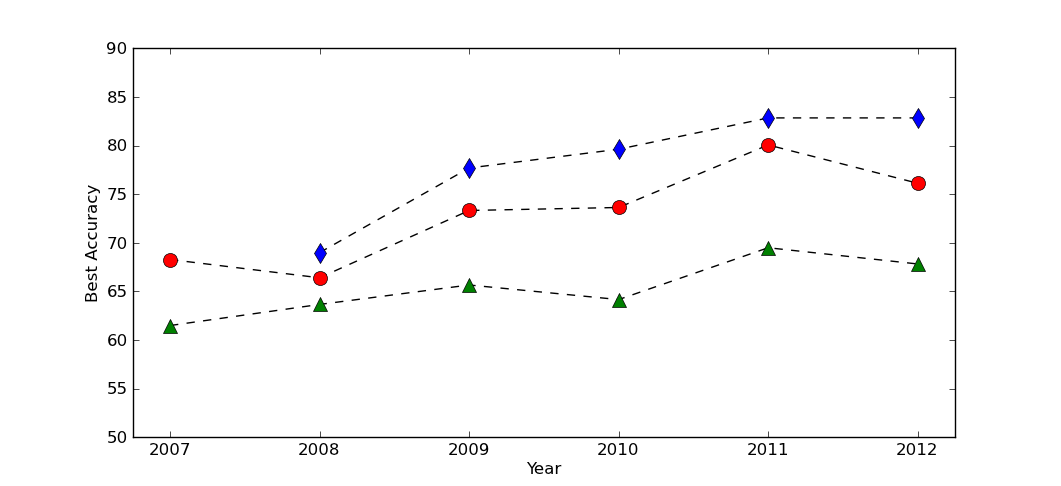
\includegraphics[width=\textwidth]{mirex2}
\caption{\emph{Losing Steam}: The best performing systems at MIREX since 2007 are plotted as a function of time for Chord Estimation (blue diamonds), Genre Recognition (red circles), and Mood Prediction (green triangles).}
\label{fig:mirex}
\end{centering}
\end{figure}

Recent research has additionally demonstrated that when state-of-the-art algorithms are used in more realistic conditions, i.e. larger datasets, performance degrades substantially \cite{BertinMahieux2012Largescale}.
Others have gone as far as to challenge the very notion that any progress has been made at all, due to issues of problem formulation and validity \cite{Sturm2014State}.
While the truth of the matter likely falls somewhere between ``erroneous results'' and ``sound science'', these varied observations encourage a critical reassessment of content-based music informatics.
Does content \emph{really} matter, especially when human-provided information has proven to be more useful than representations derived from the content itself \cite{Slaney2011Webscale}?
If so, what can be learned by analyzing recent approaches to content-based analysis \cite{Flexer2012MIREX}?
Do applications in content-based music informatics lack adequate formalization and rigorous validation \cite{Sturm2014Kiki}?
Is the community considering all possible approaches to solve these problems \cite{Humphrey2012Moving}?

Building on the premise that automatic music description is indeed valuable, this chapter is an attempt to answer the remainder of these questions.
Section \ref{sec:common} critically reviews conventional approaches to content-based analysis and identifies three major deficiencies of current systems:
one, the sub-optimality of hand-designing features;
two, the limitations of shallow architectures;
and three, the short temporal scope of conventional music signal processing.
Section \ref{sec:deep_learning} then introduces the ideas of deep architectures and feature learning in terms of music signal processing, two complementary approaches to system design that may alleviate these issues, and surveys the application of these methods in this domain.
Finally, Section \ref{sec:discussion} summarizes the concepts covered herein, and discusses why it is critical point in time for the music informatics community to consider alternative approaches.


\section{Reassessing Common Practice in Automatic Music Description}
\label{sec:common}

Despite a broad spectrum of application-specific problems, the vast majority of music signal processing systems adopt a common two-stage paradigm of feature extraction and semantic interpretation.
Leveraging substantial domain knowledge and a deep understanding of digital signal theory, researchers carefully architect signal processing systems to capture useful signal-level attributes, referred to as \emph{features}.
These signal features are then provided to a pattern recognition machine for the purposes of assigning semantic meaning to observations.
% TODO: Fill in URLs.
Crafting good features is a particularly challenging subproblem, and it is becoming standard practice amongst researchers to use precomputed features\footnote{Million Song Dataset} or off-the-shelf implementations\footnote{MIR Toolbox, Chroma Toolbox, MARSYAS, Echonest API}, focusing instead on increasingly more powerful pattern recognition machines to improve upon prior work.
While early research mainly employed simple classification strategies, such as nearest-neighbors or peak-picking, recent work makes extensive use of sophisticated and versatile techniques, e.g. Support Vector Machines \cite{Mandel2005Song}, Bayesian Networks \cite{Mauch2010Approximate}, Conditional Random Fields \cite{Sumi2012Music}, and Variable-Length Markov Models \cite{Chordia2011Predictive}.
% TODO: Fix this figure.
\begin{figure}
\begin{centering}
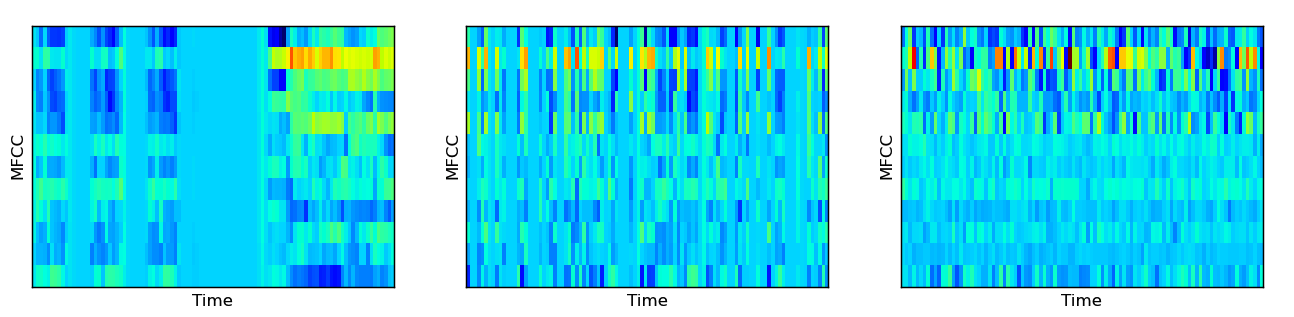
\includegraphics[width=\textwidth]{mtb_mfccs}
\caption{\emph{What story do your features tell?} Sequences of MFCCs are shown for a real music excerpt (left), a time-shuffled version of the same sequence (middle), and an arbitrarily generated sequence of the same shape (right). All three representations have equal mean and variance along the time axis, and could therefore be modeled by the exact same distribution.}
\label{fig:mfccs}
\end{centering}
\end{figure}

This trend of squeezing every bit of information from a stock feature representation is suspect because the two-tier perspective hinges on the premise that \emph{features are fundamental}.
Such representations must be realized in such a way that the degrees of freedom are informative for a particular task; features are said to be \emph{robust} when this is achieved, and \emph{noisy} when variance is misleading or uninformative.
The more robust a feature representation is, the simpler a pattern recognition machine needs to be, and vice versa.
It can be said that robust features \emph{generalize} by yielding accurate predictions of new data, while noisy features can lead to the opposite behavior.

% Traditionally, the community has placed a high value on the development of ``good'' features, supported by the sizeable body of literature on feature design and the convergence to a handful of common representations.
To illustrate the notion of quality in acoustic features, consider the scenario presented in Figure \ref{fig:mfccs}.
Conceptually, the generic approach toward determining acoustic similarity between two music signals proceeds in three stages: short-time statistics are computed to characterize acoustic texture, e.g. Mel-Frequency Cepstral Coefficients (MFCCs); the likelihood that a feature sequence was drawn from one or more probability distributions is measured, e.g. a Gaussian Mixture Model (GMM); and finally, a distance is computed between these representations, e.g. KL-divergence, Earth mover's distance, etc. \cite{Berenzweig2004Large}.
Importantly, representing time-series features with summary statistics discards temporal structure.
Therefore, the three feature sequences shown ---a real excerpt, a shuffled version of it, and a randomly generated one with the same statistics--- are identical in the eyes of such a model.
The audio that actually corresponds to these respective representations, however, will certainly not \emph{sound} similar to a human listener.

This bears a significant consequence: any ambiguity introduced or irrelevant variance left behind in the process of computing features must instead be resolved by the pattern recognition machine.
Previous research in chord estimation has explicitly shown that better features allow for simpler classifiers \cite{Cho2010Exploring}, and intuitively many have spent years steadily improving their respective feature extraction implementations \cite{Lyon2010Sound,Mueller2011Chroma}.
Moreover, there is ample evidence these various classification strategies work quite well on myriad problems and datasets \cite{Bishop2006Pattern}.
The logical conclusion to draw from this observation is that underperforming automatic music description systems are more likely the result of deficiencies in the feature representation than the classifier applied to it.

It is particularly prudent then, to examine the assumptions and design decisions incorporated into feature extraction systems.
In music signal processing, audio feature extraction typically consists of a recombination of a small set of operations, as depicted in Figure \ref{fig:simplearch}: splitting the signal into independent short-time segments, referred to as blocks or frames; applying an affine transformation, generally interpreted as either a projection or filterbank; applying a point-wise nonlinear function; and pooling across frequency or time.
These operations can be, and often are, repeated in the process.
For example, MFCCs are computed by filtering a signal segment at multiple frequencies on a Mel-scale (affine transform), taking the logarithm (a nonlinearity), and applying the Discrete Cosine Transform (another affine transformation).
Similarly, chroma features are produced by applying a constant-Q filterbank (affine transformation), taking the complex modulus of the coefficients (nonlinearity), and summing across octaves (pooling).

\begin{figure}[t]
\begin{centering}
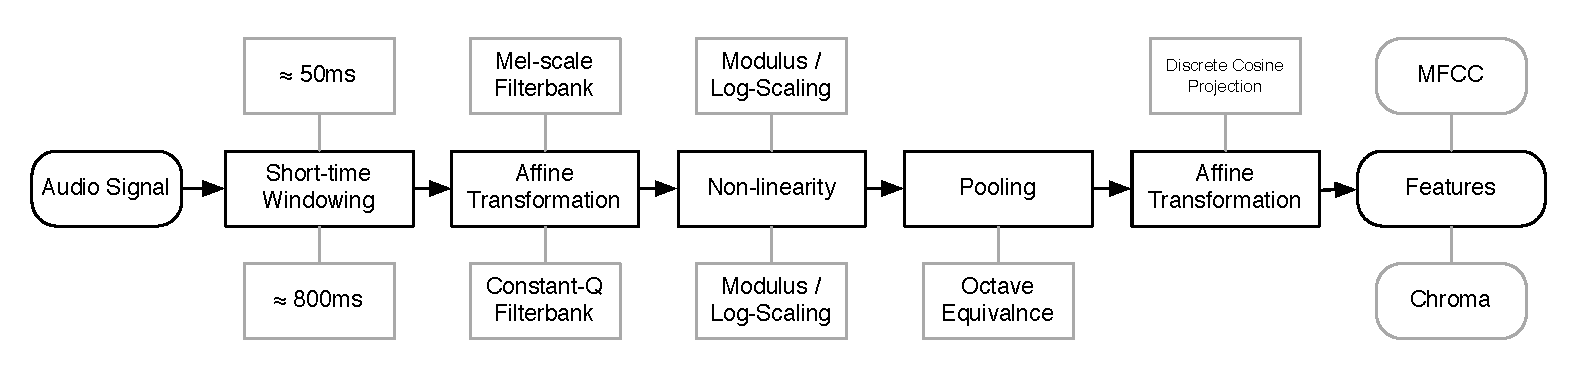
\includegraphics[width=\textwidth]{simplearch}
\caption{\emph{State of the art}: Standard approaches to feature extraction proceed as the cascaded combination of a few simpler operations; on closer inspection, the main difference between chroma and MFCCs is the parameters used.}
\label{fig:simplearch}
\end{centering}
\end{figure}


Considering this formulation, there are three specific reasons why this approach might be problematic.
First, though the data-driven training of classifiers and other pattern recognition machines has been standard for over a decade in music informatics, the parametrization of feature extractors ---e.g. choice of filters, nonlinearities and pooling strategies, and the order in which they are applied--- remains, by and large, a manual process.
Both feature extraction and classifier training present the same basic problem: there exists a large space of possible signal processing systems and, somewhere in it, a configuration that optimizes an objective function over a dataset.
Though the music informatics community is privileged with a handful of talented researchers who are particularly adept at exploring this daunting space, crafting good features can be a time consuming and non-trivial task.
Additionally, carefully tuning features for one specific application offers no guarantees about relevance or versatility in another scenario.
As a result, features developed for one task are used in others for which they were not specifically designed.
The caveat of repurposing features designed for other applications is that, despite potentially encouraging results, they have yet to be optimized for this new use case.
Good features for chord estimation may blur out melodic contours, for example, and this information might be particularly useful for structural analysis.
In fact, recent research has demonstrated that better features than MFCCs exist for speech recognition \cite{Mohamed2011Deep}, the very task for which they were designed, so it is reasonable to assume that there are better musical features as well.
The conclusions to draw from this are twofold: continuing to manually optimize a feature representation is not scalable to every problem, and the space of solutions considered may be unnecessarily constrained.


Second, these information processing architectures can be said to be \emph{shallow}, i.e. incorporating only a few nonlinear transformations in their processing chain.
Sound is a complex phenomenon, and shallow processing structures are placed under a great deal of pressure to accurately characterize the latent complexity of this data.
Feature extraction can thusly be conceptualized as a function that maps inputs to outputs with an order determined by its \emph{depth}; for a comprehensive discussion on the merits and mathematics of depth, we refer the curious reader to \cite{Bengio2009Learning}.
Consider the example in Figure \ref{fig:curvefit}, where the goal is to compute a low-dimensional feature vector (16 coefficients) that describes the log-magnitude spectrum of a windowed violin signal.
One possible solution to this problem is to use a \emph{channel vocoder} which, simply put, low-pass filters and decimates the spectrum, producing a piece-wise linear approximation of the envelope.
It is clear, however, that with only a few linear components we cannot accurately model the latent complexity of the data, obtaining instead a coarse approximation.
Alternatively, the \emph{cepstrum} method transforms the log-magnitude spectrum before low-pass filtering.
In this case, the increase in depth allows the same number of coefficients to more accurately represent the envelope.
Obviously, powerful pattern recognition machines can be used in an effort to compensate for the deficiencies of a feature representation.
However, shallow, low-order functions are fundamentally limited in the kinds of behavior they can characterize, and this is problematic when the complexity of the data greatly exceeds the complexity of the model.

\begin{figure}[t]
\begin{centering}
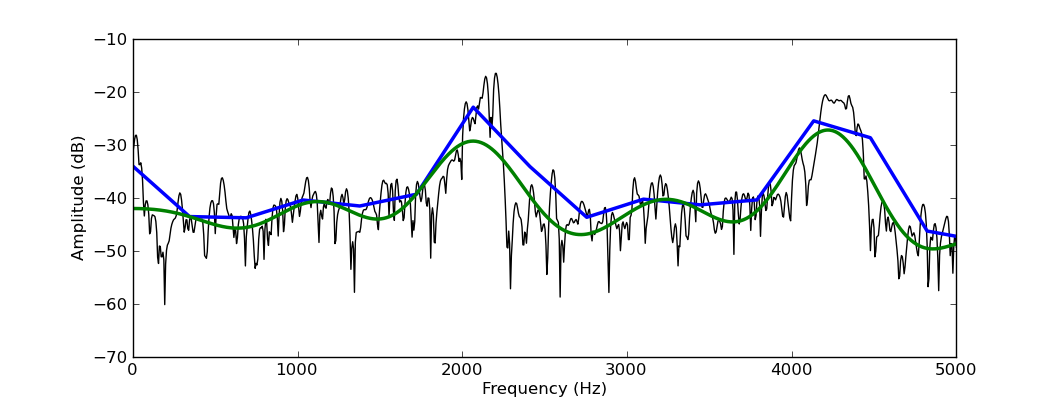
\includegraphics[height=1.5 in]{specfit}
\caption{\emph{Low-order approximations of highly nonlinear data}: The log-magnitude spectra of a violin signal (black) is characterized by a channel vocoder (blue) and cepstrum coefficients (green). The latter, being a higher-order function, is able to more accurately describe the contour with the same number of coefficients, i.e. smaller mean-squared error.}
\label{fig:curvefit}
\end{centering}
\end{figure}

Third, short-time signal analysis is intuitively problematic because the vast majority of our musical experiences do not live in hundred millisecond intervals, but at least on the order of seconds or minutes.
Conventionally, features derived from short-time signals are limited to the information content contained within each segment.
As a result, if some musical event does not occur within the span of an observation ---a motif that does not fit within a single frame--- then it simply cannot be described by that feature vector alone.
This is clearly an obstacle to capturing high-level information that unfolds over longer durations, noting that time is extremely, if not fundamentally, important to how music is perceived.
Admittedly, it is not immediately obvious how to incorporate longer, or even multiple, time scales into a feature representation, with previous efforts often taking one of a few simple forms.
\emph{Shingling} is one such approach, where a consecutive series of features is concatenated into a single, high-dimensional vector \cite{Casey2008Analysis}.
Also known as tiles, patches, or windows, shingled representations show promise by incorporating longer-term information, but incur a linear increase in dimensionality which can pose a number of challenges in practice.
Alternatively, \emph{bag-of-frames (BoF)} models produce summary statistics over feature shingles, fitting the observations to a probability distribution.
As addressed earlier with Figure \ref{fig:mfccs} though, bagging features discards temporal structure, such that any permutation of the feature sequence yields the same distribution.
The most straightforward technique is to ignore longer time scales at the feature level altogether, relying on post-filtering \emph{after} classification to produce more musically plausible results.
For this to be effective though, the musical object of interest must live at the time-scale of the feature vector or it cannot truly be encoded.
Ultimately, the question of how to process music signals over longer time-scales remains an open research topic.



\subsection{A Concise Summary of Current Obstacles}
\label{subsec:obstacles}
In an effort to understand why progress in content-based music informatics may be plateauing, the standard approach to music signal processing and feature design has been reviewed, deconstructing assumptions and motivations behind various decisions.
As a result, three potential areas of improvement are identified.
So that each may be addressed in turn, it is useful to succinctly restate the main points of this section:

\begin{itemize}

\item \textbf{Hand-crafted feature design is neither scalable nor sustainable}: Framing feature design as a search in a solution space, the goal is to discover the configuration that optimizes an objective function. Even conceding that some gifted researchers might be able to achieve this on their own, they are too few and the process too time-consuming to realistically solve every feature design challenge that will arise. \\
\item \textbf{Shallow processing architectures struggle to describe the latent complexity of real-world phenomena}: Feature extraction is similar in principle to compactly approximating functions. Real data, however, lives on a highly nonlinear manifold and shallow, low-order functions have difficulty describing this information accurately. \\
\item \textbf{Short-time analysis cannot naturally capture higher level information}: Despite the importance of long-term structure in music, features are predominantly derived from short-time segments. These statistics cannot capture information beyond the scope of its observation, and common approaches to characterizing longer time scales are ill-suited to music.\\

\end{itemize}

\section{Deep Learning: A \emph{Slightly} Different Direction}
\label{sec:deep_learning}

Looking toward how the research community might begin to address these specific shortcomings in modern music signal processing, there is an important development currently underway in computer science.
\emph{Deep learning} is riding a wave of promise and excitement in multiple domains, toppling a variety of long-standing benchmarks \cite{Krizhevsky2012Imagenet,Hinton2012Deep}, while slowly permeating the public lexicon \cite{Brumfiel2014Deep,Markoff2012Scientists}.
Despite all the attention, however, this approach to solving machine perception problems has yet to gain significant traction in content-based music informatics.
Before attempting to formally define deep learning, though, it is useful to break down the ideas behind the very name itself and develop an intuition as to why this area is of particular interest.


\subsection{Deep Architectures}
\label{subsec:deep_architectures}

It was previously shown that deeper processing structures are better suited to characterize complex data.
Such systems can be difficult to design, however, as it can be challenging to decompose an abstract music intelligence task into a logical cascade of operations.
That said, the evolution of tempo estimation systems is a perfect example of a deep signal processing structure that developed naturally in the due course of research.

The high-level design intuition behind a tempo tracking system is relatively straightforward and, as evidenced by various approaches, widely agreed upon.
First, the occurrence of musical events, or onsets, are identified, and then the underlying periodicity is estimated.
The earliest efforts in tempo analysis tracked symbolic events \cite{Dannenberg1984Online}, but it was soon shown that a time-frequency representation of sound was useful in encoding rhythmic information \cite{Scheirer1998Tempo}.
This led to in-depth studies of onset detection \cite{Bello2005Tutorial}, based on the idea that ``good'' impulse-like signals, referred to as \emph{novelty functions}, would greatly simplify periodicity analysis.
Along the way, it was also discovered that applying nonlinear compression to a novelty function produced noticeably better results \cite{Klapuri2006Analysis}.
Various periodicity tracking methods were simultaneously explored, including oscillators \cite{Large1994Resonance}, multiple agents \cite{Goto1995Realtime}, inter-onset interval histograms \cite{Dixon2007Evaluation}, and tuned filterbanks \cite{Grosche2011Extracting}.

% TODO: Redo this fig!
\begin{figure}
\begin{centering}
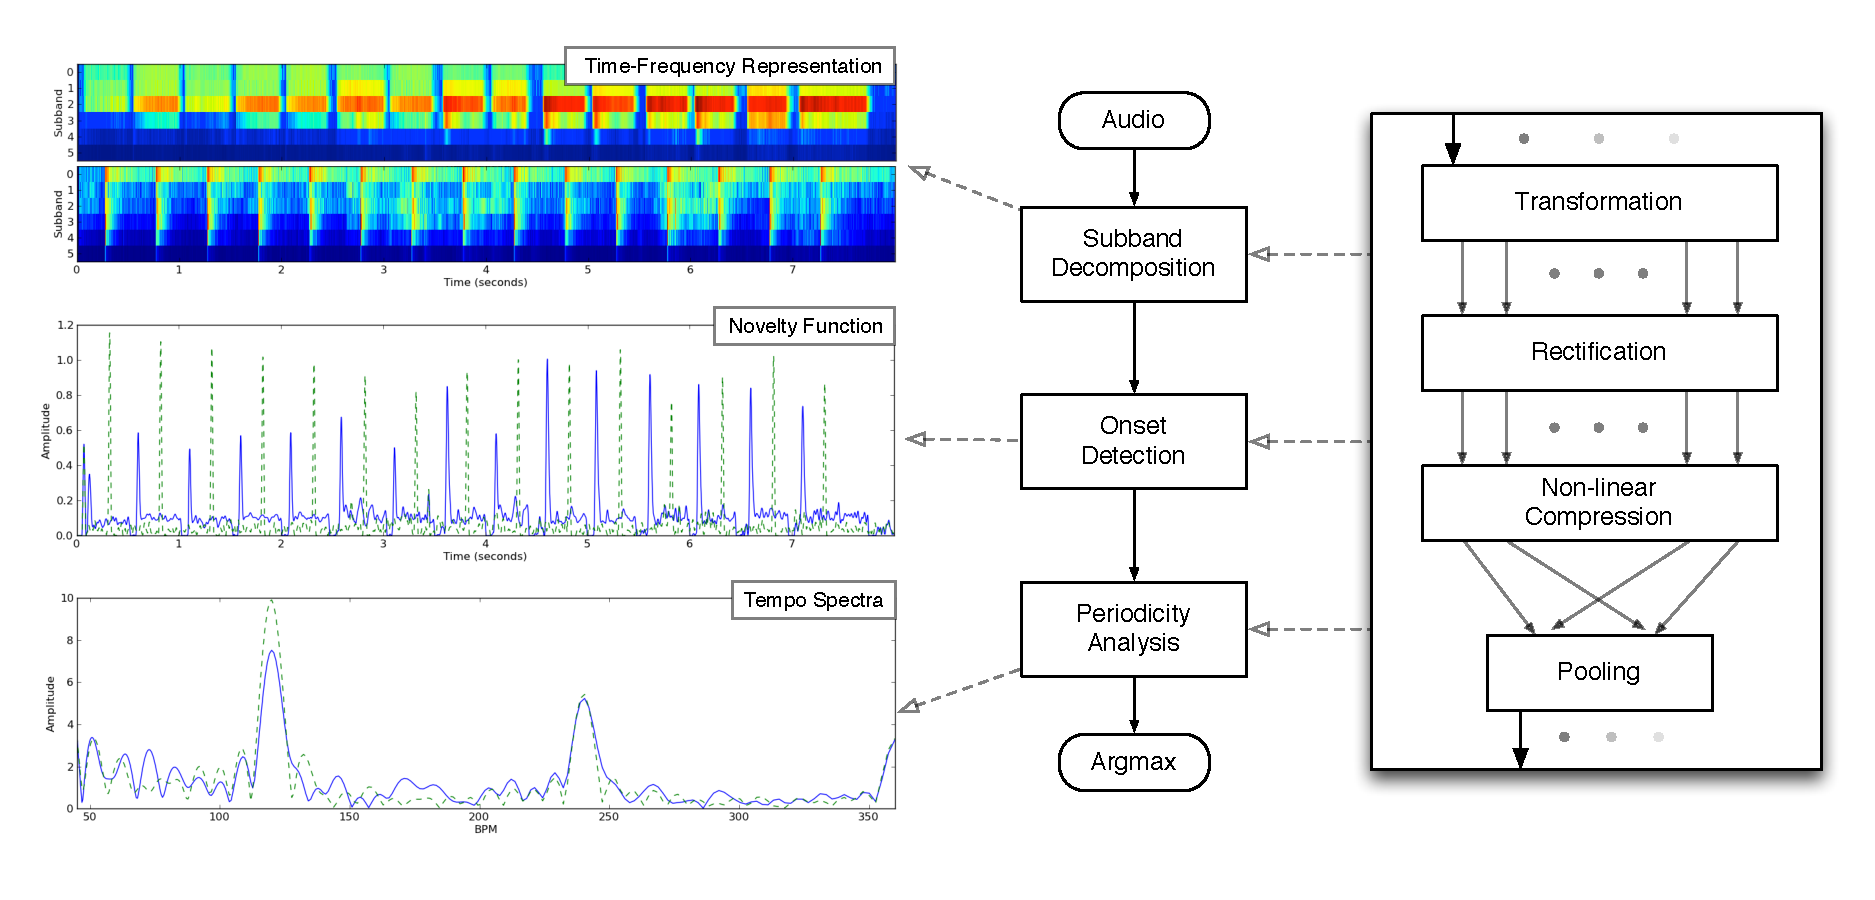
\includegraphics[width=\textwidth]{hierarchicaltecture}
\caption{\emph{A complex system of simple parts}: Tempo estimation has, over time, naturally converged to a deep architecture. Note how each processing layer absorbs a different type of variance ---pitch, absolute amplitude, and phase--- to transform two different signals into nearly identical representations.}
\label{fig:hierarchicaltecture}
\end{centering}
\end{figure}

Reflecting on this lineage, system design has, over time, converged to a deep learning architecture, minus the learning, where the same processing elements ---filtering and transforms, nonlinearities, and pooling--- are replicated over multiple processing layers.
Interestingly, as shown in Figure \ref{fig:hierarchicaltecture}, visual inspection demonstrates why it is particularly well suited to the task of tempo estimation.
Consider two input waveforms with little in common but tempo; one, an ascending D Major scale played on a trumpet, and the other, a delayed series of bass drum hits.
It can be seen that, at each layer, a different kind of variance in the signal is removed.
The filterbank front-end absorbs rapid fluctuations in the time-domain signal, spectrally separating acoustic events.
This facilitates onset detection, which provides a pitch and timbre invariant estimate of events in the signal, reducing information along the frequency dimension.
Lastly, periodicity analysis eliminates shifts in the pulse train by discarding phase information.
At the output of the system, these two acoustically different inputs have been transformed into nearly identical representations.
Therefore, the most important lesson demonstrated by this example is how invariance can be achieved by distributing complexity over multiple processing layers.

As mentioned, not all tasks share the same capacity for intuition.
Multi-level wavelet filterbanks, referred to as scattering transforms, have also shown promise as a general deep architecture for audio classification by capturing information over not only longer, but also multiple, time-scales \cite{Anden2011Multiscale}.
Recognizing MFCCs as a first-order statistic, this second-order system yielded better classification results over the same observation length while also achieving convincing reconstruction of the original signals.
The authors demonstrate their approach to have conceptual parallels with MFCCs, and exhibit strong parallels to certain deep network architectures, although the parameterization here is not learned but defined.
Perhaps a more intriguing observation to draw from this work though is the influence a fresh perspective can have on designing deep architectures.
Rather than propagating all information upwards through the structure, the system keeps summary statistics at each timescale, demonstrating better performance in the applications considered.


\subsection{Feature Learning}
\label{subsec:feature_learning}

In traditional music informatics systems, features are tuned manually, leveraging human insight and intuition, and classifiers are often tuned automatically, leveraging an objective criterion and numerical optimization.
For this reason, the quality of hand-crafted features is a crucial aspect of system design, as numerical optimization occurs downstream of manual feature design.
Many are well aware of the value inherent to good representations, and feature tuning has become a common, if tedious, component in music informatics research.
One such instance where this has occurred is in the tuning of chroma features.
Developed by Fujishima around the turn of the century \cite{Fujishima1999Realtime}, the last decade and a half has seen consistent iteration and improvement on the same basic concept; estimate the contribution of each pitch class over a short-time observation of audio.
Though initially devised for chord estimation, chroma features have been used in a variety of applications, such as structural segmentation \cite{Levy2007Comparison} or version identification \cite{Salamon2013Tonal}.

The fundamental goal in computing chroma features is to consolidate the energies of each pitch class according to a particular magnitude frequency representation.
One of the simplest ways to do so, given in Figure \ref{fig:all_weights}-(a), shows the averaging of pitch classes in a constant-Q filterbank, e.g. frequencies are spaced like the keys of a piano.
Later developments found that weighting the contributions of each frequency with a Gaussian window led to better performance, as shown in Figure \ref{fig:all_weights}-(b) \cite{Cho2014Improved}.
This improvement still took time to develop, further motivating the notion that other simple modifications remain undiscovered.
That said, this knowledge is attained by maximizing a known objective measure, such as classification accuracy in a chord estimation task.
Reflecting, this begs an obvious question: perhaps the parameters of a chroma estimation function could instead be \emph{learned} via numerical optimization?

\begin{figure}
\begin{centering}
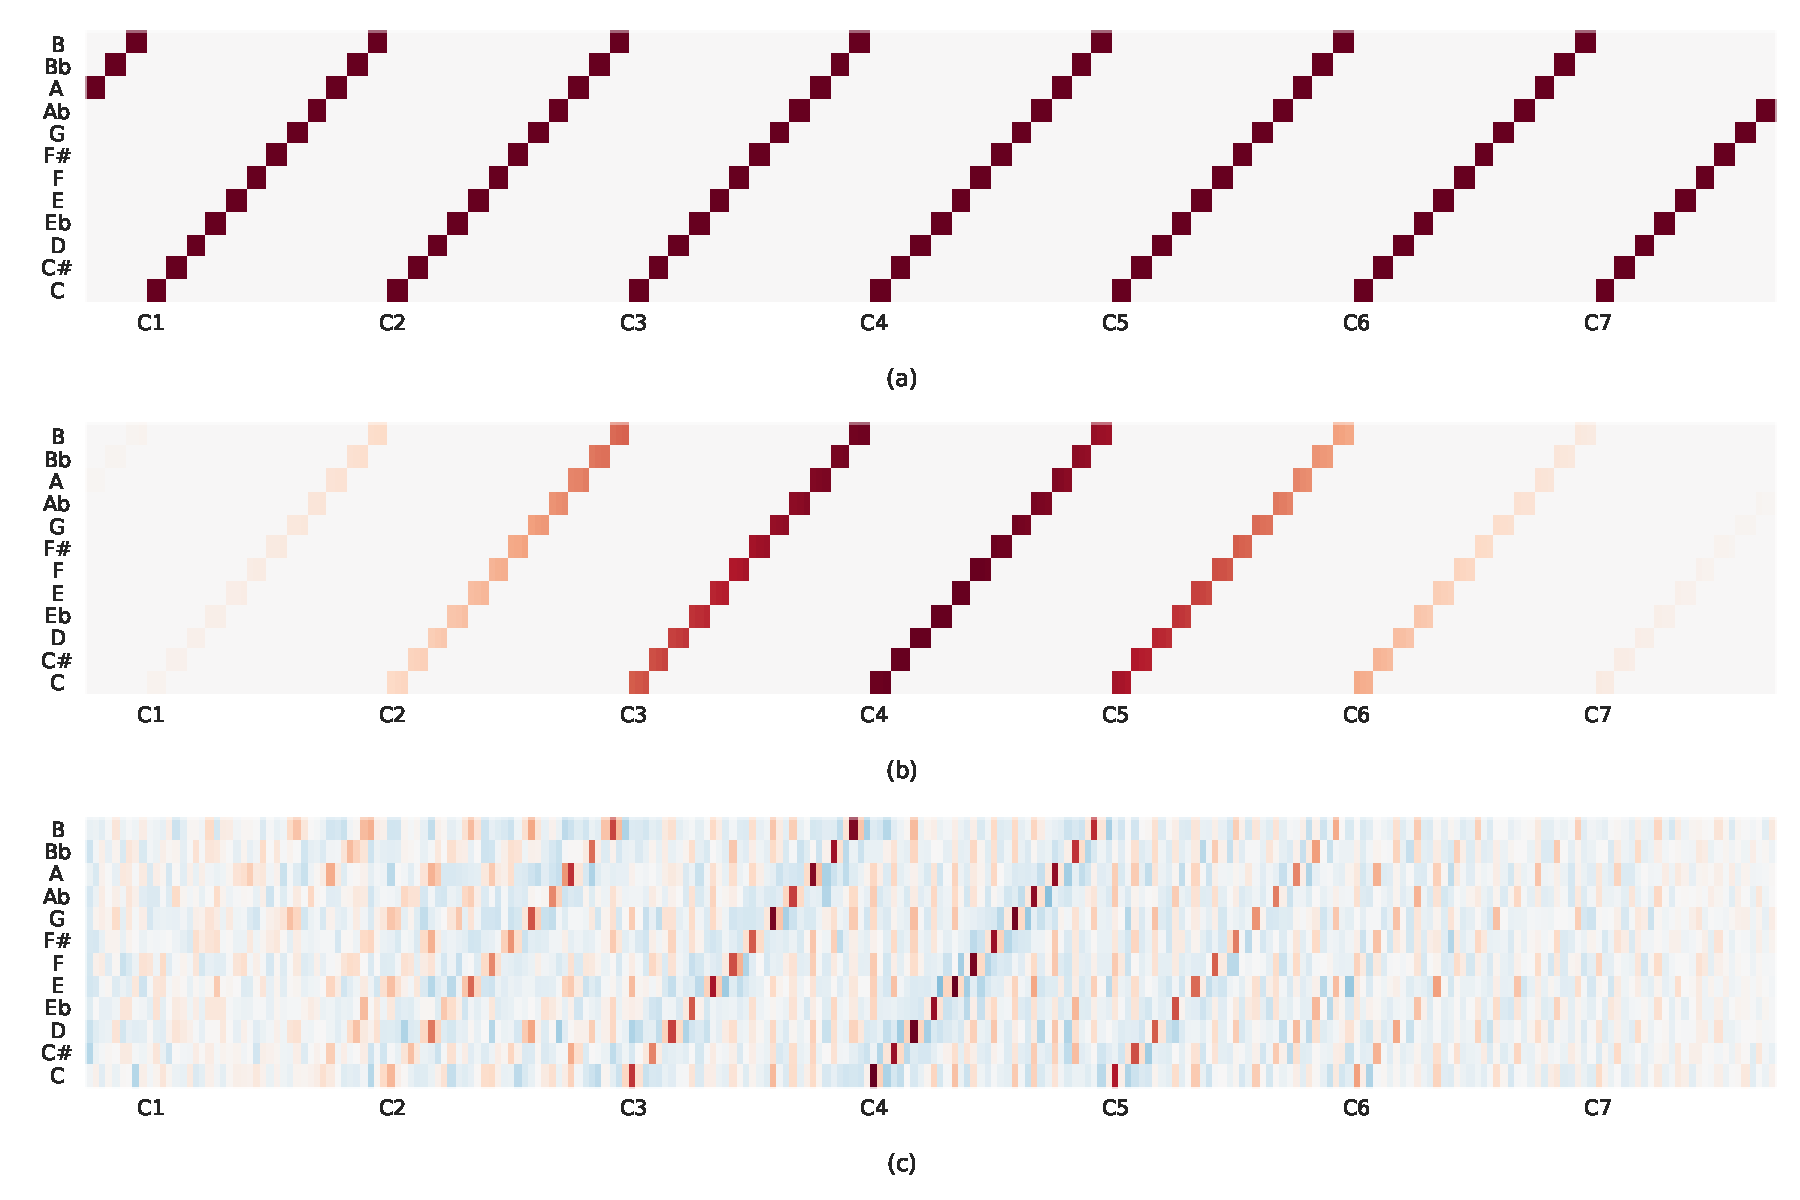
\includegraphics[width=\textwidth]{all_weights}
\caption{Various weight matrices for computing chroma features, corresponding to (a) uniform average, (b) Gaussian-weighted average, and (c) learned weights; red corresponds to positive values, blue to negative.}
\label{fig:all_weights}
\end{centering}
\end{figure}

Using the same general equation, a linear dot product between pitch spectra and a weight matrix, the mean-squared error is minimized between estimated chroma features and idealized ``target'' chroma features.
Reference chord transcriptions are used as an information source for the target chroma, producing binary templates from the chord labels.
The resulting weight matrix is illustrated in Figure \ref{fig:all_weights}-(c), and exhibits three significant behaviors.
First, the positive contributions to each pitch class are clearly seen at the octaves, as to be expected.
Second, the learned features corroborate the idea that the octave contributions should be weighted by a windowing function, and the one here looks vaguely Gaussian.
Third, and most importantly, the learned weights exhibit a small amount of suppression around each octave, shown in blue.
Similar to a Ricker wavelet \cite{Vaidyanathan1993Multirate}, negative sidebands serve to diminish wideband regions of energy, like those that are found in percussion.


\begin{figure}
\begin{centering}
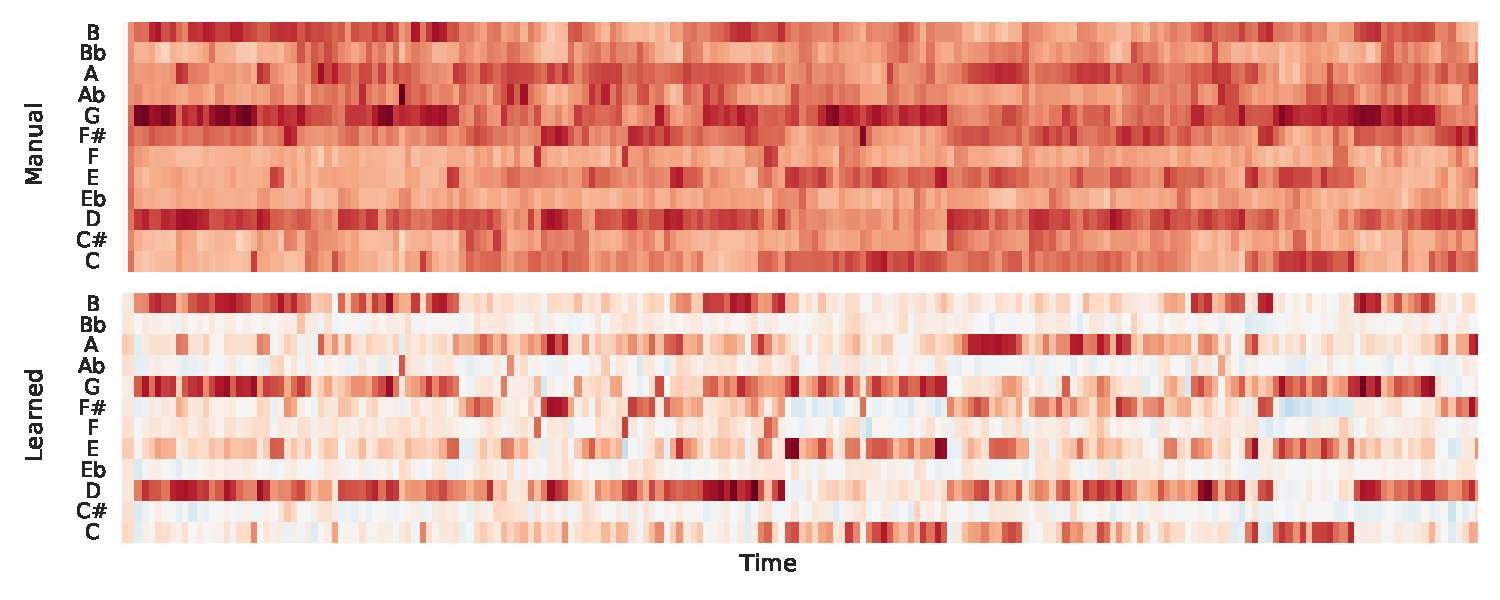
\includegraphics[width=\textwidth]{learned_chroma_TRAOIOP149E3AD2F51}
\caption{Comparison of manually designed (top) versus learned (bottom) chroma features.}
\label{fig:learned_chroma}
\end{centering}
\end{figure}

The chroma features obtained by these last two methods, (b) and (c), are shown in Figure \ref{fig:learned_chroma}.
The dynamic range of the learned chroma features is greater than that of the hand-crafted variant, as a direct result of the negative suppression in the learned weights.
While the idea of adjacent pitch energy suppression is novel, it is important to recognize a few things about this example.
Most importantly, it is curious to consider what other design aspects ``learning'' might help tease out from data.
The function considered here, a linear dot product, is very constrained, and ``better'' features are likely possible through more complex models.
Additionally, it is possible to directly inspect the learned weights because the system is straightforward; more complex models, however, will make this process far more difficult.


\subsection{Previous Feature Learning Efforts in Music Informatics}

While far from widespread, an increasing number of researchers have begun investigating deep learning to challenges in content-based music informatics.
% MLPs, DBNs
The most common form of deep learning explored for music applications focuses on such models to single frames of a music signal for genre recognition \cite{Hamel2009Automatic}, mood estimation \cite{Schmidt2011Modeling}, note transcription \cite{Nam2011Classification}, and artist recognition \cite{Dieleman2011Audio}.
% Convolutional networks
Meanwhile, the earliest instance of modern deep learning methods applied to music signals is found in the use of convolutional networks for the detection of onsets \cite{Lacoste2007Supervised}.
More recently, convolutional networks have also been explored for genre recognition \cite{Li2010Automatic}, instrument similarity \cite{Humphrey2011Nonlinear}, chord estimation \cite{Humphrey2012Learning, Humphrey2012Rethinking}, onset detection \cite{Schluter2014Improved}, and structural segmentation \cite{Ullrich2014Boundary}.
% TODO: Battenberg.
% Recursive models
Recursive neural networks, a powerful, if troublesome, model for sequential data, have also found success in chord transcription \cite{Boulanger2013Audio} and polyphonic pitch analysis \cite{Sigtia2014RNN}.
Additionally, predictive sparse decomposition (PSD) and other methods inspired by sparse coding have also seen a spike in interest \cite{Henaff2011Unsupervised, Nam2012Learning}, but while they make use of learning, neither of these systems are particularly deep.
% TODO: Discuss Independent components analysis (who?), non-negative matrix factorization (Paris, Emmanulle et al), sparse coding (Gael, Smith / Lewicki / Nam).
Regardless, it is worthwhile to note that many, if not all, of these works have attained state of the art performance on their respective tasks, often in the first application of the method to the area.

% Symbolic?
% Beyond the space of audio signal processing, deep networks have also been used in to model symbolic music information.
% Conditional networks were demonstrated rhythm pattern analysis \cite{Battenberg2012}.
% Long short-term memory to model symbolic music sequences \cite{Eck2008}.
% Multiple viewpoint for similarity \cite{Cherla2014}


\section{Discussion}
\label{sec:discussion}

Recognizing the potential for performance plateaus across various application areas in content-based music informatics, this chapter has attempted to develop an understanding as to why this might be the case.
Revisiting common approaches to the design of music signal processing systems revealed three possible shortcomings:
manual feature design cannot scale to every problem the field will need to solve;
many architectures are too shallow to adequately model the complexity of the data;
and the challenge of incorporating longer time-scales remains an open question.

In looking to other related disciplines, it seems deep learning may help address some, if not all, of these issues.
Deep architectures are able to distribute complexity across multiple processing layers, thus being able to model more complex data.
Feature learning, on the other hand, allows for the automatic optimization of known objective functions, making it easier to discover signal-level characteristics relevant to a given task faster.
In fact, a handful of previous deep learning efforts within music informatics have already begun to demonstrate the promise of such methods.

Notably, these are crucial observations to make now for a variety of reasons.
From a practical standpoint, many in the research community are investing considerable effort in the curation of datasets.
While some, like \cite{Bittner2014Medleydb}, have gone to great lengths to clear licenses for the source audio signals, most use commercial recordings and thus sharing the original content is problematic.
As a result, it is becoming standard practice to apply a respected, but non-invertible, feature extraction algorithm over the original audio content and share the extracted statistics with the community, e.g. the Million Song Dataset \cite{Bertin2011Million}.
While these efforts are commendable, such datasets are ultimately limited by the feature extraction algorithm employed.

As a final comment, this is not to imply that feature design is intrinsically deficient, but rather an acknowledgment of the reality that feature extraction is somewhat by definition a lossy process;
thus, essential information to solve some task may be inadvertenly discarded as a result.
It is only fair to recognize that some degree of representation engineering can be adventageous in the application of deep learning to music signal processing.
The goal of representation design in these two scenarios, however, is quite different:
whereas conventional feature design attempts to ultimately solve the problem, representation design for deep learning, as we will see, strives to make the problem easier to solve.
While this does not preclude the latter from being non-trivial, there is a larger margin for error as uncertainty can be deferred to the learning stage.


% this file is called up by thesis.tex
% content in this file will be fed into the main document

%: ----------------------- introduction file header -----------------------
% the code below specifies where the figures are stored
\graphicspath{{3/figures/}}

\chapter{Deep Learning}
\label{chp:background}
% This article is structured very well: http://www.toptal.com/machine-learning/an-introduction-to-deep-learning-from-perceptrons-to-deep-networks
% Goals:
%  - Provide contextual background for deep networks (how did we get here)
%  - Equate traditional digital signal processing and deep learning
%  - Define the necessary pieces of deep learning

% Outline
%  - Background
%   -- Origins
%   -- Breakthroughs
%   -- State of the Art / recent developments
%  - Formal Definitions
%   -- What is ``deep learning''; non-linear function, parameterized, differentiable, optimized to a given objective criterion.
%   -- Architectures
%    --- Affine Layers
%    --- Convolutions (2d, 3d)
%    --- Nonlinearities
%    --- Pooling
%   -- Energy-based Learning
%    --- Scalar objective criteria (Loss Functionals)
%    --- Stochastic Minibatch Gradient Descent
%   -- Tricks
%    --- Regularization & Sparsity
%    --- Parameter Initialization
%    --- Dropout
%    --- Data Augmentation
%  - Relationship to Audio DSP


Deep learning descends from a long and contested history of artificial intelligence, information theory, and computer science.
The goals of the this chapter are two-fold:
Section \ref{background} first offers a concise summary of the history of deep learning in three parts, detailing the origins, critical advances, and current state of the art of neural networks.

Afterwards, a formal treatment of deep learning is addressed:
Section \ref{sec:arch} introduces the architectural components of deep networks;
Section \ref{sec:learning} formally addresses the actual ``learning'' process;
Section \ref{sec:tricks} covers a handful of pertinent tricks of the trade, enabling the practical realization of such models;
and finally, Section \ref{sec:dsp} draws the relationships between this lineage and conventional approaches to digital signal processing.


\section{A Brief History of Neural Networks}

Despite the recent wave of interest and excitement surrounding it, the core principles of deep learning were originally devised halfway through the 20th century, and grounded in mathematics established even earlier.
A direct descendant of the now-infamous neural network, the very mention of deep learning often ellicts several justified questions: What's the difference? What's changed? Why \emph{now}?
Thus, before delving into a formal treatment of the topic, it is worthwhile to contextualize the research trajectory that led to this point.
% For this reason is particularly valuable to consider the lineage of these methods in an effort to understand why it is only now that such approaches have begun to gain popularity and scientific acclaim.


\subsection{Origins (pre-1980)}
\label{subsec:origins}

For Western Europe and those in its sphere of influence, the Age of Enlightenment marked a golden era of human knowledge, consisting of great advances in many diverse fields, such as mathematics, philosophy, and the physical sciences.
Long had humanity contemplated the notions of consciousness and reasoning, but here brilliant thinkers began to return to and explore these concepts with resolve.
From the efforts of scholars like Gottfried Leibnitz, Thomas Hobbes, and George Boole, formal logic blossomed into its own mathematical discipline.
In doing so, it became possible to symbolically express the act of reasoning, whereby rational thought could be described by a system of equations to be transformed or even solved.

It was this critical development ---the idea of logical computation--- that encouraged subsequent generations to speculate on the apparent feasibility of artificial intelligence.
And, coinciding with the advent of electricity in the 20th century, mathematicians, philosophers, and scientists of the modern era sought to create machines that could \emph{think}.
While the space of relevant contributions is too great to enumerate here, there were a handful of breakthroughs that would prove integral to the field of computer science.
In 1936, Alan Turing devised the concept of a ``universal machine'', which would lead to the proof that a system of binary states, e.g. true and false, could be used to perform \emph{any} mathmatical operation \cite{Turing1936}.
Only a year later, Claude Shannon demonstrated in his \emph{master's} thesis that Boolean logic could be implemented in electrical circuits via switches and relays, forming the basis of the modern computer \cite{Shannon1937}.
Shortly thereafter, in 1943, Pitts and McCulloch constructed the first artifical neuron, a simple computational model inspired by discoveries in neuroscience \cite{Pitts1943}.
By coarse analogy to a biology, an artifical neuron ``fires'' when a weighted combination of its inputs eclipses a given threshold, e.g. 0:

% \begin{align*}
% f(x | w) = h( \mathbf{w}^T \dot \mathbf{x}) \\
% h(y) = \left\{
%      \begin{array}{lr}
%        1 : y \ge 0\\
%        0 : y < 0\\
%      \end{array}
%    \right.
% \end{align*}

\begin{align*}
  f(x~|~w) = h(w^T~\cdot~x)\\
  h(y) = \left\{
    \begin{array}{ll}
      1 : y \ge 0\\
      0 : y < 0\\
    \end{array}
  \right.
\label{eq:perceptron}
\end{align*}

\noindent Importantly, as shown in Figure \ref{fig:neuron_logic}, it was demonstrated that such a model could be used to reproduce Boolean operations, such as AND or OR.
Given the clear application to the field of computational logic, artifical neurons only further encouraged the pursuit of artificially ``intelligent'' machines.

% Perceptron!
On its own, an artifical neuron is only a general processing structure, and the parameters it takes will specify the precise behavior of the model.
Arriving at these parameters, however, was nontrivial and required manual derivation.
Thus, in 1957, Frank Rosenblatt's invention of the \emph{Perceptron} algorithm signficantly altered how artificial neurons were conceived \cite{Rosenblatt1957}.
Building upon the work of Pitts and McCulloch, the algorithm, given in \ref{alg:perceptron_fit}, offered an automated method of ``learning'' the parameters necessary to achieve binary classification over a collection of data:

% \begin{algorithm}
% % \caption{Fit a Perceptron to a collection of data.}
% \label{alg:perceptron_fit}
% \begin{algorithmic}[1]
% \Procedure{fit}{$\mathbf{x}, \mathbf{y}, \nu, n_{max}$}
%     \State $\mathbf{w} \gets \mathcal{N}(\mu, \sigma)$
%     \State $n \gets 1$
%     \While $\sum~|e| > 0$ or $n > n_{max}$
%         \State $\mathbf{z} = f(\mathbf{x} | \mathbf{w})$
%         \State $\mathbf{e} = \mathbf{z} - \mathbf{y}$
%         \State $\mathbf{w} \gets \mathbf{w} + \nu (\mathbf{e}^T \dot \mathbf{x})^T$
%         \State $n \gets n + 1$
%     \EndFor
%     \State Return $\mathbf{w}$
% \EndProcedure
% \end{algorithmic}
% \end{algorithm}

\begin{algorithm}[H]
\caption{Compute sum of integers in array}
\label{array-sum}
\begin{algorithmic}[1]
\Procedure{ArraySum}{$A$}
    \State $sum = 0$
    \For {each integer $i$ in $A$}
        \State $sum = sum + i$
    \EndFor
    \State Return $sum$
\EndProcedure
\end{algorithmic}
\end{algorithm}

\noindent First, the weights, $\mathbf{w}$, are set to some initial condition.
Then, in an iterative manner, outputs, $\mathbf{z}$, are predicted from the inputs, $\mathbf{x}$, and the weights are updated with a scaled version of the incorrectly classified inputs.
Note that the error vector, $\mathbf{e}$ is only non-zero where the predicted values are wrong, and thus the algorithm ceases execution when all datapoints are classified correctly, or it reaches some number of iterations.
A visual example of this is given in Figure \ref{fig:linsep}.
Here, a perceptron is used to separate two classes of data, drawn from different Gaussian distributions.
As the algorithm proceeds, the total error decreases until a decision boundary is found that correctly classifies all datapoints.

\begin{figure}
\begin{centering}
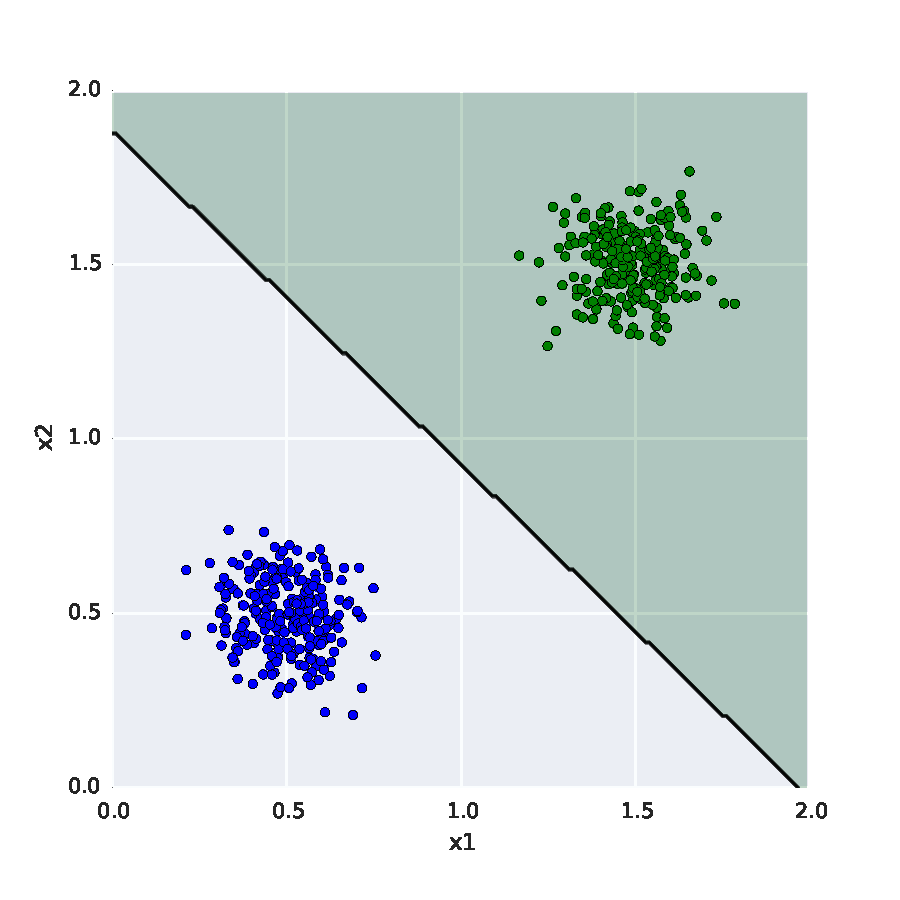
\includegraphics[width=0.6\textwidth]{linsep}
\caption{Linearly separable data classified by a trained perceptron.}
\label{fig:linsep}
\end{centering}
\end{figure}

% Promise and limitations
Once implemented in hardware, using a slew of potentiometers, motors, and photocells, Rosenblatt's' ``Mark I Perceptron'' drew considerable attention from the press and the research community alike.
The \emph{New York Times} was quick to publish ambitious claims as to the promise this breakthrough held for artificial intelligence and the speed at which subsequent advances would be realized, much to the chagrin of the AI community \cite{somebody}.
% The Perceptron was not without limitations
In their book, \emph{Perceptrons}, published in 1969, Minsky and Papert demonstrated that the model is rather limited in the functions it can reproduce.
As such, perceptrons could only be used to classify linearly separable conditions, and not more complex operations, such as the exclusive-or (XOR).
This condition is illustrated in Figure \ref{fig:mlp_ftw}, where no single line can be draw to correctly classify the data.

% Multilayer Perceptrons
This was a critical limitation for researchers in the field of computational logic; if a perceptron could not perform a simple exclusive-or, how could a machine be expected to reason?
The answer, as it would turn out, could be found by transforming how the XOR is expressed symbolically.
Rearranging terms, an equivalent function can be rewritten as the disjuction (OR) of two complementary conjuctions (AND):

\begin{equation}
\label{eq:xor}
p \oplus q = (p \wedge \neg q) \vee (\neg p \wedge q)
\end{equation}

\noindent While it is true that a single Perceptron cannot achieve this operation directly, a combination of \emph{three} can: two are used to perform each AND operation and corresponding negation, while a third performs the OR operation.
Considering the scenario in Figure \ref{fig:mlp_ftw}, this condition can now be easily separated by a \emph{multilayer} perceptron (MLP).
Therefore, arbitrarily complex functions could be obtained by cascading simpler non-linear operations, in what would be commonly reffered to as a \emph{neural network}.
In fact, it would later be shown by the \emph{universal approximation theorem} that a neural network is actually able to model \emph{any} continous function within some tolerance \cite{Cybenko1989, Hornik1991}.

\begin{figure}
\begin{centering}
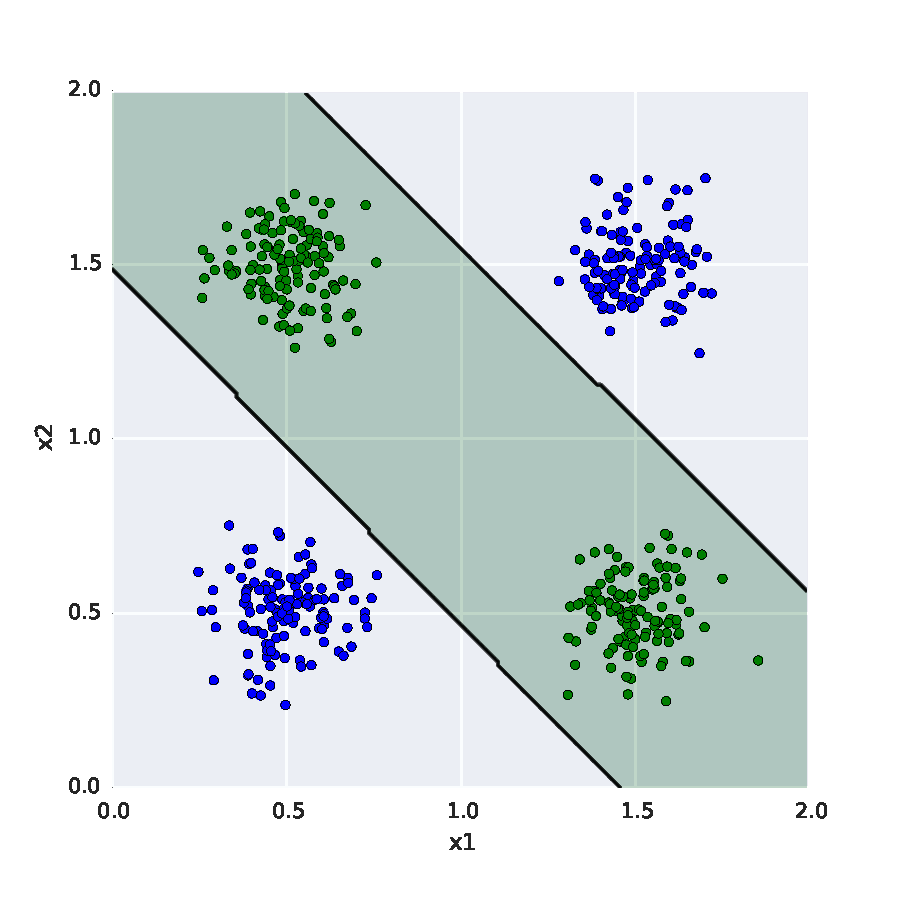
\includegraphics[width=0.6\textwidth]{mlp_ftw}
\caption{Demonstration of the decision boundaries for a \emph{multi-layer} perceptron.}
\label{fig:mlp_ftw}
\end{centering}
\end{figure}

% Other problems
Despite this observation, the study of neural networks languished through the closing decades of the 20th century, suffering a considerable downtick of interest and funding support.
While the representational power of multilayer perceptrons was recognized early on, many often claimed ---incorrectly--- that they could not be used to solve complex problems.
More practically, those who continued to pursue neural network research were faced with an array of other challenges.
Neural networks were prone to over-fitting, extremely slow to compute weight updates over a large number of datapoints, and difficult to train with more than a few layers.
% Ahead of the times
% Theory outpaced technological capacity. Over-hyped
In isolation, these issues might merely have a posed a standard research obstacle, but coupled with the failed promises of overzealous researchers, such difficulties would malign neural network research for some time.
% This resulted in what is affectionately known as one of the ``AI winter'', things got bad.


\subsection{Scientific Milestones (1980--2010)}
\label{sec:advances}

Despite widespread pessimism toward neural computing, a select few would persevere through this ``AI Winter''.
Over the course of thirty odd years, these diligent efforts would yield a array of crucial breakthroughs and fundamentally change the landscape of neural network research.
While no single contribution can truly be credited with reviving the field, each would play an integral role in helping the research community warm up to neural networks.

\subsubsection{Stochastic Gradient Descent}
\label{subsec:sgd}

% Back-propagation of errors
Via the perceptron algorithm, a machine effectively ``learns'' to classify data by finding parameters that optimize a given objective function.
Originally this was framed as a minimization, as in Eq. \ref{eq:perceptron}, such that the error, known as the ``perceptron loss'', could be incrementally decreased by taking small steps toward better parameters.
This optimization strategy must be modified in the multilayer case, as it is not possible to directly update the parameters through the heaviside, or unit step, function.
Early researchers noted that if the discontinuous activation function is replaced with a logistic, or sigmoid, the composite multilayer network is \emph{differentiable}.
The derivative of each coefficient, regardless of layer, can be computed with respect to the loss, thus \emph{back-propagating} error through the network \cite{Hinton1986}.

% Issues of gradient descent
Error back-propagation demonstrated that, so long as a network was everywhere differentiable, it was theoretically possible to optimize the objective function over a dataset by slowly adjusting parameters towards better solutions.
This optimization method, referred to as \emph{gradient descent}, was not without its deficiencies, however.
First and foremost, the loss of a given configuration was typically computed over the entire dataset, which may prove computationally expensive for sufficiently large collections.
Additionally, gradient descent is a greedy search algorithm, and was reportedly prone to finding poor local minima, as illustrated in Figure \ref{fig:local_min}.

%Stochastic Gradient Descent
In 1987, however, LeCun demonstrated that a \emph{stochastic} variant of gradient descent could potentially be used to circumvent these issues \cite{LeCun1987}.
Whereas conventional gradient descent had been formulated as an optimization over an entirely collection of datapoints, this new version randomly sampled training samples from a collection and computed an update step based on single datapoint.
Though the gradient is much noiser, this strategy is still effective,significantly faster, and may even be less susceptible to poor local minima as a result.
Importantly, this notion can be generalized as \emph{mini-batch} gradient descent, where the number of datapoints used to compute parameter updates is a hyperparameters, varying from 1 to the total number of datapoints available for training.
Covarying inversely with the learning rate, illustrated in Figure \ref{fig:sgd}, larger batch sizes serve to smooth parameter updates as a function of iteration.

\subsubsection{Convolutional Neural Networks}
\label{subsec:convnets}

% Fully connected networks, bleh; sensitive to translation and scale
% TODO: Needs a better context sentence

Though equal parts remarkable and encouraging, the universal approximation theorem says nothing about how one might parameterize a neural network to achieve some desired behavior.
Thus, despite such overwhelming promise, early neural networks often resulted in poor approximations of the functions being modeled, because the flexibility of the model vastly surpassed the amount of data available to train it.
This flexibility was apparent in computer vision tasks, as multilayer perceptrons struggled to cope with simple homographic deformations, such as translation, scaling, or rotation.

% Visual cortex, neocognitron
Natural vision systems, on the other hand, are quite robust to these kinds of variation, and, as before, researchers looked to biology for inspiration in modeling these processes.
One particularly crucial study was that of Hubel and Wiesel in 1959, who experimented on the neural behavior of the feline visual cortex \cite{}.
By presenting visual stimuli while probing the brain with electrodes, they discovered two different kinds of neurons ---simple cells and complex cells--- organized hierarchically.
Experimental results indicated that the former is responsible for local feature extraction, while the latter combines the inputs of simple cells to absorb small amounts of variation in the observed stimuli.

% ConvNets, LeNet5, handwritten digits
These ideas were first incorporated in the Neocognitron of \cite{Fukushima1988}, and realized successfully as a convolutional neural network, or ``ConvNet'', for shape recognition and handwritten digit classification \cite{LeCun1990, LeCun1998}.
Importantly, ConvNets incorporated three key design features.
\emph{Local receptive fields}, where compute features from a small neighborhood of pixels, exploiting the observation that nearby pixel values tend to be highly correlated.
Smaller receptive fields require fewer parameters, thus reducing the overall size of the model and the amount of data needed to train it.
Applying local receptive fields as a convolution results in effectively sharing the weights over all positions in an image.
Thus \emph{weight sharing} reduces the number of parameters even further, while allowing the network to identify features regardless of position in an image.
Finally, \emph{max-pooling} reduces small neighborhoods to the largest value within it, introducing not only shift but a small amount of scale and rotation invariance.
Taken together, these advantageous attributes directly resolved many of the issues plaguing multilayer perceptrons, and proved to be the most successful instance of neural computing for nearly two decades.


% Theory preceded data
\subsubsection{Proliferation of Digital Data}
\label{subsec:perceptrons}

% Proliferation of digital content
During the first rise and fall of neural networks, digital data was far more the exception than the rule.
Digitized audio and images didn't become common until the end of the 20th century.
Even so, the data rate of these signals made processing them computationally prohibitive: ata
The internet, conceived in the 1960s, didn't rise to public prominence in the US until the 1990s.

% Labeled datasets grew, intentionally or otherwise
Researchers had time to build large labeled datasets.
Along with the internet, it became possible to use weakly labeled data or distribute the annotation effort.
MNIST is the hallmark of curated datasets.
TIMIT for speech
CAPTCHA for optical character recognition.
ImageNet, GWAP.
Weakly labeled data from the internet, researchers got clever.

% unlabeled data has uses too
Finally in 2006, one such method, called contrastive divergence was proven successful, using a slightly different processing model known as a Restricted Boltzmann machine (RBM).
The important characteristic of an RBM is that it can be used to generate, as well as process, information in both directions.
This is fundamental to contrastive divergence, which trains each layer of a deep network separately by learning to recreate its input data.
By analogy, this approach aims to discover structure in the data that occurs with high probability and effectively ``ignore'' everything else.
When strung together as a full network, these systems are referred to as deep belief networks (DBNs), as a result of their probabilistic formulation.
Subsequently, a similar model called an autoencoder \cite{Vincent2010}, or ---an alternative interpretation from another research team--- Predictive Sparse Decomposition \cite{Ranzato2007}, incorporates roughly the same principles with deterministic interpretation of these concepts.
In either view of the parameter optimization problem, learning algorithms now exist that can leverage large quantities of unlabeled data to tune large networks with minimal supervision.
These advances have collectively ushered in a new era of machine learning, referred to as \emph{deep learning}, named so for the multiple levels of information processing and the manner in which the parameters of the system are discovered from data.


% Theory preceded technology
\subsubsection{Advances in Computing Technology}
\label{subsubsec:hardware}

% Neural networks were devised in the 60s; in the 80s, computers sucked
While enough cannot be said about the scientific contributions of neural network researchers over the last 40 years, it is critical to appreciate how computing technology has evolved over that time span.
In the days of Rosenblatt and Minsky, computers consisted of transistors that were visible to the naked eye, filled entire rooms, and cost a small fortune.
More recently, personal computers of the 1980s had kilobytes of memory, central processing units (CPUs) operated in the range of tens of megahertz, and were still far too expensive for all but the elite or dedicate.
Computation was still quite slow as a result, and thus the process of traning neural networks took an impressive amount of time.
To combat these difficulties, researchers often attempted to cut corners by using smaller models, smaller datasets, and training with fewer iterations.
Somewhat unsurprisingly, the common experience with neural networks was quite unfavorable.

% Now better; bigger hard disks, more memory, faster processors, GPUs, async SGD, distributed computing, better tools (Theano, Torch)
Eventually, though, technology could catch up to the theory.
Hardware became increasingly smaller, memory grew to the size of gigabytes, processors accelerated for a time without bound faster, and the cost of computers dropped to the point of near ubiquity.
On the heels of these developments, other hardware and tools were adapted to facilitate neural network research, such as parallel computing with graphics processing units (GPUs) and accessible software tools, e.g. Theano\footnote{} or Torch\footnote{}.
Combined, singificantly better technology directly enabled research at unprecedented scale, accelerating progress and relaxing computational constraints imposed by technical limitations.

% Additionally, significant increases in computational power, and especially advances in parallel computing via GPUs, make deep learning not only feasible, but in some cases an efficient approach to research.
% Evidenced by the recent work of \cite{kittehs}, some are beginning to attempt large scale deep learning on unprecedented quantities of data.
% Similarly, software libraries and toolkits \cite{Theano, Torch, Caafe} are now available that leverage these computational gains to make deep learning more accessible to the entire research community.


\subsection{Modern Rennaissance (post-2010)}
\label{subsec:rennaissance}

Industrial strength; Google, Facebook, Baidu, Microsoft
Press; YouTube and Cats, Yann LeCun, Geoff Hinton, IEEE, NYTimes
Competitions: Kaggle, Netflix, ImageNet


\section{Core Concepts}
\label{sec:example}

% The "what" of deep learning
At the highest level, deep learning is an approach to nonlinear system design that combines high level function design with numerical optimzation in an effort to model some observable behavior.


Having covered the ``why'' of deep learning, this section aims to generalize the concepts of classic neural computation into a more general presentation of its fundamental components.



\subsection{Modular Architectures}
\label{subsec:architectures}

S'all fair game so long as you can differentiate it.

\subsubsection{Linear Algebra}

% Fully connected / affine
Conventionally, a neural network transforms an input $X_{1}$ into an output $Z_{L}$ via a composite nonlinear function $F(\cdot \vert \Theta)$, given a parameter set $\Theta$.
This is traditionally achieved as a cascade of $L$ simpler nonlinear functions $f_l(\cdot \vert \theta_l)$, referred to as layers, the order of which is indexed by $l$:

\begin{equation}
\label{eq:layers}
F(X_{1} \vert \Theta) = f_{L}(  ... f_2(f_1(X_{1} \vert \theta_1) \vert \theta_2) ) ... \vert \theta_{L})
\end{equation}

\noindent In this formulation, $F = [f_1, f_2, ... f_{L} ]$ is the set of layer functions, $\Theta = [\theta_1, \theta_2, ... \theta_{L} ]$ is the corresponding set of layer parameters, the output of one layer is passed as the input to the next, as $X_{l+1} = Z_{l}$, and the overall \emph{depth} of the network is given by $L$.


While a layer $f_l$ can be any differentiable function, we limit our focus in this work to fully-connected, or \emph{affine}, transformations, defined by the following:

\begin{equation}
\label{eq:fclayer}
f_l(X_l \vert \theta_l) = h( W \bullet X_{l} + b), \theta_l = [W, b]
\end{equation}

\noindent Here, the input $X_l$ is flattened to a column vector of length $N$ and the dot-product is computed with a weight matrix $W$ of shape $(M, N)$, followed by an additive vector bias term $b$ with length $M$.
Note that an affine layer transforms an $N$-dimensional input to an $M$-dimensional output, referred to as the \emph{width} of the layer.
The final operation is a point-wise nonlinearity, $h(\cdot)$, defined here as $tanh(\cdot)$, which is bounded on $(-1, 1)$.

% Local Receptive Fields
Fully connected matrices that are only connected to local neighborhoods.
This can be generalized as a very large dot product where most parameters are fixed to zero.

% Convolutions
Same formulation as local receptive fields, except the parameters are tied across location.

% Other connectivities
Could be data driven, a la Coates et al \cite{Coates2012?}.

\subsubsection{Nonlinearities}

Logistic / sigmoid, hyperbolic tangent.
Close cousins, but generally hyperbolic tangent has gained favor for being centered about the origin.

Rectified linear, piecewise linear model. % relationship to random forests?
Results in naturally sparse representations.
Doesn't saturate in the positve region, but no information flows in the negative mode.
Leaky ReLU, gradient everywhere.

%Softmax
When used as a classification system, the first $L-1$ layers of a neural network can be viewed as feature extractors, and the last layer, $f_L$, is a simple linear classifier.
The output representation can be made to behave like a posterior by constraining the $L_1$-norm of the output to equal $1$.
Traditionally, the probability mass function $P(\cdot)$ for an input $X_1$ is achieved by applying the softmax operation to the output of the network, $Z_L$, defined as follows:

% TODO: Isn't there a Beta term here?
\begin{equation}
\label{eq:softmax}
\sigma(Z) = \frac{\exp(\beta Z)}{ \sum_{k=1}^{K}\exp{(\beta Z_k)}}
\end{equation}

\noindent Again, note that $Z$ is the output of the final layer, $f_L$, and thus $K$ is the dimensionality of the classifier and equal to the number of classes in the problem.
Therefore, the most likely class for a prediction $Z$, is given by $k = argmax(\sigma(Z))$.

Notably, any differentiable nonlinearity could conceivably be used here.


\subsubsection{Pooling}

Max pooling is the most common form, usually applied to a local neighborhood.
Also L2 variant
Relationship to max-out networks.


\subsection{Energy-based Learning}

Ideally, these features are \emph{learned} automatically using what are known as gradient methods, the basic idea being that a function attempts to reduce how ``wrong'' it is by taking small steps toward better answers; by analogy, this is a bit like climbing down a mountain blind-folded.
For this to be possible, the activation of each node, as expressed in Equation (\ref{eq:perceptron}), must be softened such that the function is differentiable.


Having written the full network as a probability mass function, the network can be trained by iteratively minimizing the negative log-likelihood of the correct class for a set of $K$ observations:

\begin{equation}
\label{eq:nll}
\mathcal{L}=-\sum_{k=0}^K log(P(X^k = Y^k \vert \Theta))
\end{equation}

\noindent Expressed in this manner, $X^k$ and $Y^k$ are the input data and corresponding class label, respectively of the $k^{th}$ observation.

We can then minimize this loss function via mini-batch stochastic gradient descent.
Here, gradients are computed with $K>1$, but much smaller than the total number of observations, by sampling datapoints from the training set and averaging the loss over the batch.
Specifically, the update rule for $\Theta$ is defined as its difference with the gradient of the scalar loss $\mathcal{L}$ with respect to the parameters $\Theta$, weighted by the learning rate $\eta$, given by the following:

\begin{equation}
\label{eq:updaterule}
\Theta \leftarrow \Theta - \eta * \frac{ \delta \mathcal{L}}{\delta \Theta}
\end{equation}


\subsection{Tricks of the Trade}
\label{subsec:tricks}

%   -- Tricks
\subsubsection{Regularization \& Sparsity}
Reduce over-fitting via weight decay.
L2 penalties make values small without going to zero

Sparse representation are good.
L0 and L1 loss are closely related, will drive values all the way to zero.

\subsubsection{Data-Driven Initialization}

Core idea behind the last significant breakthrough of the modern era.
Get parameters of the network closer to a good solution.
Resolves poorly conditioned networks.
Alleviates the vanishing gradient problem.

Recently it was observed that with enough data, rectified linear units, or both, this is less crucial than once thought.


\subsubsection{Dropout}
Preventing co-adaptation of parameters.
Related to model averaging.
Reduces theoretical bounds on generalization error.


\subsubsection{Data Augmentation}


\subsubsection{Bootstrapping Additional Information}
Sparse coding
Jordan Net


% Looking closely at recent work in deep learning, most of the effort has been invested in areas of static input representations, i.e. computer vision and still images.
% As evidenced by music, audio, and video, time plays an extremely important role in the way that information is conveyed.
% Though CNNs have been applied to signals with a temporal dimension \cite{LeCun1994}, recursive architectures have shown promise for addressing the problem of time and sequences in data.
% Initial efforts to train RNNs however, even with supervised methods, proved extremely challenging, with the observed phenomena manifesting as numerical stability issues of the gradient.
% Due to the recursive nature of the model, backpropagating the error signal through time is prone to make the amplitude of the gradient either vanish or explode.
% Despite these difficulties, several approaches and optimization methods have been developed in recent years that encourage further exploration of these models.

% One of the earliest successful attempts to circumvent the issue of gradient stability was realized through a method called LSTM \cite{Schmidhuber1997}, where the gradient signal is ``latched'' by a hidden unit such that its information could be saved long enough to be useful.
% Similar notions surround the notion of reservoir computing, such as echo-state networks, which employ feedback connections to cache arbitrary temporal information such that a second non-recursive layer ---being far easier to train--- might be able to make sense of it \cite{Jaeger2002}.
% Alternatively, conditional DBNs have been employed to model, classify, and generate convincing sequences of human motion \cite{JMLR2011}, and can be thought of as a probabilistic CNN.
% Recent research has found that more complex optimization methods are sufficient to train RNNs directly without changing the underlying model \cite{Martens2010}, giving encouraging qualitative results on motion \cite{Sutskever2008} and text generation \cite{Sutskever2011}.
% There has also been initial work investigating discriminative recursive models that also leverage unsupervised training \cite{Rolfe2013}.
% This research is particularly exciting, as it demonstrates that such models are actually within reach.
% Reflecting on the corpus of deep learning work in the past decade however, it should be noted that the majority of these breakthroughs ignore audio, and even more so music, signals, focusing instead on vision or natural language processing tasks.


\section{Previous Efforts in Automatic Music Description}

This realization is beginning to spread throughout the MIR community, and there is, understandably, an increasing interest in the application of deep learning methods to these problems.
Among the first uses of deep learning were the application of CNNs to the detection of onsets \cite{Lacoste2007} and long short-term memory to model symbolic music sequences \cite{Eck2008}.
Deep Belief Networks quickly gained popularity for genre recognition \cite{Hamel2009}, mood estimation \cite{Schmidt2011}, note transcription \cite{Nam2011}, and artist recognition \cite{Dieleman2011}, but somewhat surprisingly many of these methods operate on single, short-time observations of the music signal.
Incorporating longer time-scales, CNNs have also been used to classify inputs on the order of seconds for, again, genre recognition \cite{Li2010}, instrument classification \cite{Humphrey2010} and chord estimation \cite{Humphrey2011, Humphrey2012b}.
Predictive Sparse Decomposition (PSD) and methods inspired by sparse coding have also seen a spike in activity over the last two years for a variety of tasks \cite{Henaff2011, Nam2012}, but despite being developed for deep learning, neither of these systems are actually hierarchical.

% It is worthwhile to note that many, if not all, of these works have achieved state of the art performance on their respective tasks, often in the first application of the method to the area.
% Any instances where this has occurred, however, deep learning techniques have simply been directly some kind of derived audio representation with minimal modification.
% It is therefore important to realize that these methods have never been tailored to address the nuances of music signals, and more importantly time.
% Overall, only CNNs make an effort to consider observations on the order of seconds, but do so in an admittedly awkward way, requiring the observation length be defined \emph{a priori}.
% The machine is ultimately limited to the amount of information it sees in its analysis, and there is obviously no fixed duration in which all musical behavior resides.

Due to advances in machine computation, there are primarily two different ways to conceptualize the design of information processing models.
One approach is based on signal theory as viewed through the lens of electrical engineering, whereas the other focuses on graphical models of artificial neural processing grounded in computer science.
Though broad topics of study in themselves, they are worth mentioning together for two crucial reasons: first, a majority of inertia developed within the field of MIR is due largely to its roots in the former; and second, it is a useful juxtaposition to form when marrying these disconnected topics.

%Electrical engineering formalized as a discipline in the middle of the $19^{th}$ century on the heels of inventions such as the telegraph and electric power distribution.

Much early work in electrical engineering stemmed from the realization that electricity could be used to represent measurable phenomena and therefore capture, store, and transmit this information.
These representations are referred to as analog signals because they use one representation ---time-varying voltage, for example--- to mirror another one ---such as a sound pressure wave--- in a continuous fashion.
It was soon discovered that not only could this information be represented via electricity, but that it was also possible to analyze and manipulate it for a variety of applications.
Heavily grounded in classic numerical analysis methods of the $17^{th}$ and $18^{th}$ centuries, these methods are referred to as signal processing.
Through experimentation in physics, scientists found that certain electromagnetic materials could be used to affect electricity in predictable ways, and when connected in an electrical circuit could be used to filter, or augment, signals.
Importantly, the need to solve signal processing systems by inspection requires that the entire system be linear and time invariant (LTI), because the violation of either property makes mathematical analysis far too difficult, if not altogether impossible.

With the advent of solid-state transistors and subsequently computers in the mid-$20^{th}$, digital representations of signals could be produced by sampling analog waveforms to be manipulated numerically, referred to as digital signal processing (DSP).
Digital signals---those that also represent some kind of real world phenomena, at least---differ from analog ones in two important aspects: the signal takes values from a finite set of discrete numbers, and these quantities are measured at precise moments in time.
Therefore, digital signals are specified by a sequence of real-valued numbers $x[n]$, rather than a generated, continuous function $x(t)$.
When this transition to numerical computation began, the effort was made to reformulate previous knowledge regarding analog signal theory and processing into the digital domain.
Similar to those in analog theory, digital filters can be expressed explicitly by a transfer function, which can be translated directly to a set of coefficients representing the linear difference equation, generically given by the following:

\begin{equation}
\label{eq:diffeq}
\begin{array}{rcr}
y[n] & = & b_0x[n] + b_1x[n-1] + b_2x[n-2] + b_3x[n-3] \ldots \\
 & & - a_1y[n-1] - a_2y[n-2] - a_3y[n-3] \ldots
\end{array}
\end{equation}

There are typically said to be two categories of digital filters: Finite Impulse Response (FIR), or non-recursive, filters and Infinite Impulse Response (IIR), or recursive, filters.
As illustrated in Figure \ref{fig:filters}, an FIR filter is actually a special case of the more general IIR filter, where the feedback connections---the $a$-coefficients in Equation (\ref{eq:diffeq})---have all been set to zero.
Though digital filters are not constrained by the availability or precision of manufactured electrical components, they are still traditionally constrained to be LTI systems for the same reasons as their analog counterparts.
As a result, non-linear signal processing models in both the analog and digital domains are historically unpopular due to inherent challenges in the mathematical formulation.

\begin{figure}[!t]
\centering
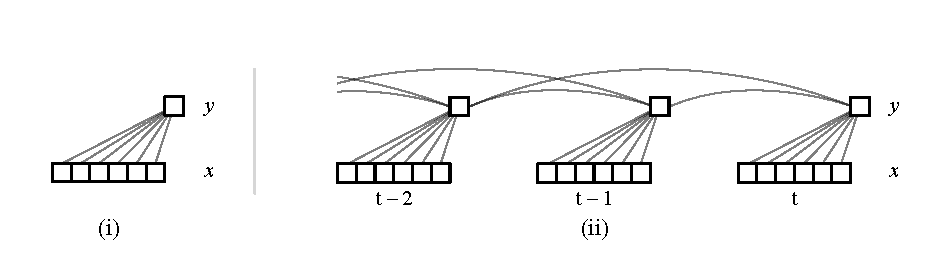
\includegraphics[width=\textwidth]{filters_2}
\caption{\small{Finite Impulse Response (i) and Infinite Impulse Response (ii) digital filters. Multiplication is shown along the edges of each connection.}}
\label{fig:filters}
\end{figure}


\section{Summary}
\label{sec:summary}

% Origins
Building upon formal logic and biological analogy, neural networks were devised in the 1960s as an approach to information processing.
However, after inital promise, they were largely met with skepticism, indifference, or worse through the remainder of the century.
% What changed?
The few who perservered made various discoveries that, coupled with steady advances in computing technology, would eventually return neural computation to the fore:
mini-batch stochastic gradient descent made optimization computationally efficient and less susceptible to poor local minima, and encouraged further exploration of numerical optimization methods;
convolutional networks reduced model complexity and over-fitting through scale and translation invariance;
and lastly, larger labeled datasets reduced overfitting, and abundant unlabeled data could be used to better initialize networks in an unsupervised manner.

Deep learning is therefore based on two principles: first, that complex problems can be decomposed into a series of simpler subproblems; and second, what exactly these simpler subproblems are or should be can be discovered from a corpus of data.


%: ----------------------- introduction file header -----------------------
% the code below specifies where the figures are stored
\graphicspath{{4/figures/}}

\chapter{Timbre Similarity}
\label{chp:timbre}

Timbre is a difficult attribute to define in acoustic perception.
Research has long sought to better understand the latent dimensions, in the hope of developing methods that can estimate the pairwise similarity between observations.
In lieu of adequate information to study this phenomenon directly, here instrument taxonomies are used as an approach to objectively define such relationships.
A non-linear semantic embedding is achieved by training a deep convolutional network to project time-frequency representations of audio into a low-dimensional, semantically organized space.
The discriminative properties of the resulting embeddings are explored, and the notions of timbral smoothness are investigated qualitatively.


\section{Context}
\label{sec:context}

% Definition
Despite its common usage in the various forms of music for centuries, a satisfactory definition of \emph{timbre} remains elusive to this day; in fact, the one adopted by the American National Standards Institute embodies this challenge, arriving at a concept through the exclusion of others \cite{ANSI197x}:

\begin{quote}
Timbre is that attribute of auditory sensation in terms of which a subject can judge that two sounds similarly presented and having the same loudness and pitch are dissimilar.
\end{quote}

%  More focus on what it isn't than what it is
As evidenced by this definition, the very notion of ``timbre'' is still an open research topic in psychoacoustics.
This reality is captured quite succinctly by Phillipe Manoury, who offered the following insight \cite{}:

\begin{quote}
One of the most striking paradoxes concerning timbre is that when we knew less about it, it didn’t pose much of a problem.
\end{quote}

% Why is this problematic
There are many advantages to developing a deeper understanding of timbre, from both an artistic and scientific perspective.
Of particular interest to this work, however, the absence of a constructive definition ---timbre is a result of X, Y, and Z--- makes it difficult to directy build computational systems to characterize and compare timbres.
Thus, before proceeding, it is valuable to review what is known of timbre, and prior efforts to transfer this knowledge into engineering systems.
% There is much to be understood about "timbre"; point is, question everything we think we know.


\subsection{Psychoacoustics}
% Historical context
% Psychoacoustics, Early work and the struggle to define
% Helmholtz, pitch, and other psychoacoustics.
%Given this inherent ambiguity in concept definition, it is worthwhile to contextualize how this situation came to be.
The perception of timbre falls under the umbrella of \emph{psychoacoustics}, a topic of study that sits at the boundary between acoustics and psychology.
Some of the earliest research in psychoacoustics was pioneered by von Helmholtz in his inquiries into the sensations of pitch and loudness \cite{Cook1995?}.
Inquiries specific to timbre would not come until much later, due to two difficulties in experimental design.
One, whereas pitch and loudness are predominantly one dimensional, it is unclear from personal introspection what the salient dimensions of timbre might be.
A subject might describe a sound as being ``brighter'' than another, but signal analysis is necessary to begin to determine why.
Additionally, researchers were limited by the kinds of stimuli they could create and use in perceptual experimentation, and thus were constrained in the space of possible parameters to explore.

% Psychology and psychoacoustics in the 1960-90s
With the advent of computers and continued scientific advances through the 20th century, these issues could be addressed directly, and several researchers set out to identify the existence of fundamental dimensions.
This work, perfomed by Plomp \cite{Plomp1976} Grey and Wessel \cite{Grey1979}, among others, adopted a similar experimental design.
Human subjects were presented pairs of sound stimuli and asked to rate the pairwise similarity between the two.
Having collected a number of ratings from a number of participants, multi-dimensional scaling was used to project the stimuli into a low-dimesional space that preserved the given relationships.
At this point, the researcher would then turn to spectral analysis to identify possible charateristics of the stimuli that might correlate with the different dimensions of the resulting projection.
This approach proved relatively fruitful, yielding a variety of signal-level statistics, or \emph{features}, found to correspond positively with subjective ratings.
Conclusions drawn from this work suggested features such as log-attack time, spectral centroid, and spectral spread, and were echoed later, as in the work of Krumhansl \cite{}.
This line of inquiry showed promise, and went on to inform much of how MIR approaches timbre and how such systems should be built.

% Deficiencies
%  - at the mercy of researcher ingenuity to find good features
%  - subjective ratings are limited by the space of stimuli used
However, more recent work identifies two issues with this approach to timbre research \cite{Glennon2014}.
First, as stated by Caclin et al., ``Given the multiplicity of acoustical parameters that could be proposed to explain perceptual dimensions, one can never be sure that the selected parameters do not merely covary with the true underlying parameters.'' \cite{Caclin2005}.
This statement can be interpreted in two related ways:
one, the space of parameters considered is bounded by the insight and ingenuity of the researcher;
and two, it is possible that a chosen parameter covaries with the true, but unobserved, parameter.
Second, the utility of a timbre space resulting from MDS is limited to the space of stimuli with which it was obtained.
In other words, factors of variance not captured by the sonic palette used as stimuli are unlikely to be encoded in the resulting dimensions.

There is also a concern regarding the degree to which conclusions resulting from research on subjective pairwise ratings might be generalized.
Typically, stimuli used in such experiements are synthetic to the point of unnatural \cite{Teresawa2007?} or chosen from a space of instrument sounds.
In the latter case, familiarity with such sounds have the potential to bias subjects away from a purely perceptual rating.
Finally, the perpection of timbre undoubtedly has a time-varying characteristic, but much research focuses on timbre as a stationary phenomena.
Some, like \cite{Krumhansl1980?}, have considered the attack and sustained regions of a sound separately, finding that instrument identification was possible from either portion.
However, by concatenating the attack of one instrument with the sustained portion of another, it was demonstrated that a subject would perceive only the attack instrument, effectively masking the signature survived in the sustain.
Such a finding illustrates that the perception of timbre not only varies over small time scales, but is dependent on context and the sequential ordering of events.

%Synthesizing this brief survey of timbre perception research into some kind of workable defintion, timbre is a time-varying quality of sound, akin to texture in the visual domain.
% Referred to by Landy as a \emph{second-order percept}, texture is the emergent property

% What are the take-aways here?
% - Previous claims of salient dimensions should be taken with a grain of salt.
% - This is why we are where we are.


\subsection{Computational Modeling}
% Computational approaches and models
% Short-time statistics
Most previous approaches to computationally modeling timbre instantaneously can be grouped into one of two categories: signal statistics and basis projections.
The first follows from the perceptual research of the later 20th century, whereby statistics representing higher level concepts are computed for their semantic merit.
Initially these corresponded to the features named by in the work of Grey or Krumhansl, but have expanded over time to include a wide array of creative and clever measures.
The interested reader is directed to \cite{Essid2006} for a comprehensive space of possible features.


% Cascaded Transforms
From an often complimentary perspective, other music researchers have designed transform-based systems to project signals into representations with various properties.
One of the earliest and most common approaches is the use of Mel-frequency Cepstral Coefficients (MFCCs) for timbre-oriented tasks.
Originally designed for speech coding purposes by Mermelstein in the 1960s \cite{Mermelstein}, the first significant contribution in MIR to call attention to these features was that of Logan in 2000 \cite{Logan}.
MFCCs have, if not in reality then at least in practice, become synonymous with timbre-centric MIR, now being used in an innumerable number of systems for instrument classification \cite{}, tagging \cite{}, genre prediction \cite{}, mood estimation \cite{} or structural analysis \cite{}, to name only a few representative works in each.
The general process of computing MFFCs is given in Figure and proceeds as follows: an input audio signal is divided into overlapping, short-time \emph{frames}, on the order of tens to hundreds of milliseconds; a filterbank, perceptually scaled in frequency, is then applied to each short-time frame and log-compressed; finally, a discrete cosine transform (DCT) is applied to these frequency coefficients, characterizing the shape of the spectrum (or the spectrum of the spectrum, referred to rather cheekily as the \emph{ceps}trum).
Often only the first dozen or so coefficients are used in practice on the principle that they capture the most relevant information, though this is more convention than rule.

% Machine learning approaches
Similar in principle, though less widely used, is to instead \emph{learn} the set of bases over which the spectrum is projected.
For exaple, the approach taken by Jehan \cite{Jehan2005}, which preserves the first 12 coefficients of a trained PCA decomposition.
In this instance, the projection into the PCA subspace attempts to decorrelate the principal axes of the data in the input space, like the Discrete Cosine Transform.
The primary difference here, however, is that the bases are learned from a sample of observations.

\subsection{Motivation}

% Motivation for similarity
While many of these approaches have proven useful in various classification tasks, none directly result in a notion of timbre similarity, a useful concept in a variety of scenarios.
The search and navigation of large sound libraries is one such instance, where sparse metadata and text-based queries often reduce the task of navigating a sound library to that of an exhaustive, brute force search.
The inherent difficulty of finding a target sound in a potentially massive collection of items lies in the inability to capture the specific query semantically, relying instead on metaphors; distorted guitars are described as `crunchy' or trumpets `bright.'

User interfaces
Composition and

\subsection{Limitations}
Failing to adopt a clear definition of timbre does not relieve you of inherently operating on one.
The work presented here is not intended to be synonomous with timbre, and is subject in many ways to the limitations named in previous perceptual research; a timbre space is achieved as a result of the inputs considered, and will likely fail on sufficiently novel stimuli.
% Additionally, you can't learn everything.


\section{Learning Timbre Similarity}
\label{sec:timbre_embedding}

From the previous review of psychoacoustics research and efforts to computationally model timbre, there are two important conclusions to draw:
first, classic timbre features are subject to the wisdom that ``corellation does not imply causation'';
and second, these features are ultimately bounded by the creativity, insight, or dilligence of a researcher.
Synthesizing these observations with the discussion from Chapter \ref{chapter:context}, there is a clear argument for feature learning in timbre-related tasks.

Having discussed the value and applications of a timbre similarity space, it is worthwhile to outline the goals for such a system.
First and foremost, one would learn, rather than design, signal-level features relevant to achieve the given task and circumvent the issues identified previously.
% This idea is based on the combination of an inability to clearly define the sensory phenomenon and the known caveats of previous perceptual studies.
Additionally, sound should be represented in an intuitive manner, such that distance between points is semantically meaningful.
In other words, signals from the same source should be near-neighbors, whereas sounds from different sources should be far apart.
% Come back to how we show this in the methodology.
Finally, the ideal similarity space is perceptually \emph{smooth}, meaning that a point that interpolates the path between two others should be a blend of the two, e.g. a tenor saxophone might fall between a clarient and a French horn.

These objectives have clear conceptual overlap with dimensionality reduction methods and instrument classification systems, on which this work builds.
The approach presented here consists of several parts, as diagrammed in Figure \ref{fig:nlse}, and discussed in the following subsections.
First, all audio is transformed into a time-frequency representation (Subsection \ref{subsec:timbre_tfr}).
The main component of the system is a deep convolutional network, which maps tiles of these time-frequency coefficients into a low-dimensional space (Subsection \ref{subsec:timbre_deepnet}).
During training, this network is duplicated such that two inputs may yield two outputs, and these parameters are learned by optimizing the distance between these two representations (Subsection \ref{subsec:timbre_pairwise}).
At test time, this pairwise harness is discarded, and the deep network is used to project inputs to the learned embedding space.


\subsection{Time-Frequency Representation}
\label{subsec:timbre_tfr}

Though it is a particular goal of the system to minimally design transformations, audio is first processed by a Constant-Q transform (CQT) for three reasons.
First, the application of a filterbank front-end results in a considerable simplification of the system, both computationally and in the number of learned parameters.
Sharing a common formulation with neural networks, a filterbank can be viewed as a hard-coded layer in the network.
Knowing the parameters in advance allows for the development of an optimized implementation, such as the one discussed in Chapter \ref{chapter:deep_learning}, reducing processing time.
Additionally, the CQT is logarithmic in frequency, serving as a reasonable approximation of the human auditory system.
Furthermore, it is generally agreed upon that timbre perception is, at least to some degree, invariant to pitch.
Also following from this earlier discussion, the use of convolutional networks allows for translation invariance of features in both $log_2$-frequency and time.

The constant-Q filterbank is parameterized as follows: all input audio is first downsampled to 16kHz; bins are spaced at 24 per octave, or quarter-tone resolution, and span eight octaves, from 27.5Hz to 7040Hz; analysis is performed at a framerate of 20Hz uniformly across all frequency bins.
Logarithmic compression is applied to the frequency coefficients with an offset of one, e.g. $log_{1p}(x) = log(x + 1.0)$.


\subsection{Deep Convolutional Networks for Timbre Embedding}
\label{subsec:timbre_deepnet}

Noting that the details of deep learning and convolutional networks are discussed at length previously, only those decisions unique to this task are addressed here; for clarity regarding the mathematical or conceptual definitions of these terms, refer to Chapter \ref{chapter:deep_learning}.

A five-layer neural network is designed to project time-frequency inputs into a low-dimensional embedding.
The first three layers make use of 3D-convolutions, to take advantage of translation invariance, reduce the overall parameter space, and act as a constraint on the learning problem.
Max-pooling is applied in time and frequency, to further accelerate computation by reducing the size of feature maps, and allowing a small degree of scale invariance in both directions.
The final two layers are fully-connected affine transformations, the latter of which yields the embedding space.
The first four hidden layers use a hyperbolic tangent as the activation function, while the visible output layer is linear, i.e. it has no activation function in the conventional sense.

Hyperbolic tangents are chosen as the activation function for the hidden layers purely as a function of numerical stability.
It was empirically observed that randomly initialized networks designed with rectified linear units instead were near impossible to train; it is hypothesized that, due to the relative nature of the learning problem, i.e. the network must discover an equilibrium for the training data, it is easy for the parameters to be pushed into a space where all activations go to zero, collapsing the network.
Conversely, hyperbolic tangents are everywhere-differentiable, and did not suffer the same behavior.
The use of activation functions that provide an error signal everywhere, such as sigmoids or ``leaky'' rectified linear units \cite{Maas2014}, or better parameter initialization might avoid this behavior, but neither were explored here.

Combining the successful application of linear ``bottleneck'' layers \cite{Liao2013} with lessons learned from previous efforts \cite{Humphrey2011}, the visible layer is chosen here to be linear.
As will be discussed in more detail shortly, a saturating nonlinearity at the output makes the choice of hyperparameters crucial in order to prevent the network from pushing datapoints against the limits of its space.
However, the absence of boundaries allows the network to find the appropriate scale factor for the embedding.

Specifically, the network is parameterized thusly: the input to the network is a 2D tile of log-CQT coefficients with shape $(20, 192)$, corresponding to time and frequency respectively; the first convolutional layer uses 20 filters with shape $(1, 5, 13)$ and max-pooling with shape $(2, 2)$; the second convolutional layer uses 40 filters with shape $(20, 5, 11)$ and max-pooling with shape $(2, 2)$; the third convolutional layer uses 80 filters with shape $(1, 1, 9)$ and max-pooling with shape $(2, 2)$; the fourth layer is fully-connected and has 256 outputs; the final layer is also fully connected, and has 3 outputs.


\subsection{Pairwise Training}
\label{subsec:timbre_pairwise}
Pairwise training
Select a distance metric
contrastive loss function
Perceptron loss + perceptron loss (margin)

Training strategy
uniform presentation + / -
minibatch stochastic gradient descent


\section{Experimental Methodology}
\label{sec:example}

Here's the explanation of what was done.

\subsection{Data}
Start with the VSL
Use instrument boundaries as a nearest neighbor taxonomy.
Cut-off at 5000 sound files.
After discarding unreasonable duplicates, left with 24 classes.
Keep three conditions from the pilo

\begin{figure}[h]
\centering

\includegraphics[width=0.6\textwidth]{pink_muffin.png}
\caption{Cupcake caramels gingerbread cake.}
\label{fig:muffin}
\end{figure}


\begin{equation}
\nabla^2p = \frac{1}{c^2} \frac{\partial^2 p}{\partial t^2}
\label{eq:wave}
\end{equation}

Muffin dragee caramels sweet pudding danish bonbon jelly-o \gls{tcap}.
Dessert chocolate bar marzipan.
Tiramisu cheesecake caramels cake lemon drops. Icing pastry lollipop marshmallow jujubes.
Gingerbread carrot cake marzipan souffle halvah. Bear claw cheesecake toffee pie donut.
Dessert pastry applicake biscuit caramels marzipan croissant muffin \ref{tab:things}.

\begin{table*}[h]
\begin{center}
\caption{Halvah danish liquorice sesame snaps}
\begin{tabular}{l l l l l l l}
Dessert & Love \\
\hline
Cookie & 5.8\\
Macaroon & 9.3\\
Sugar plum & 0.78\\
\hline
\end{tabular}
\label{tab:things}
\end{center}
\end{table*}


\noindent
Icing cheesecake biscuit pudding marshmallow.
Cake toffee fruitcake gummi bears.
Macaroon macaroon lollipop marzipan.
Ice cream tiramisu pie powder halvah.








%: ----------------------- introduction file header -----------------------
% the code below specifies where the figures are stored
\graphicspath{{5/figures/}}

\chapter{Automatic Chord Estimation}
\label{chp:chord_estimation}

% Context / Purpose
The focus of this study now turns to automatic chord estimation (ACE), one of the oldest subtopics in the field of content-based MIR.
Complementing the previous chapter, ACE presents a more challenging, well-worn problem with a long research lineage and myriad applications.
In addition to the standard objective of advancing the state of the art in a given application domain, this chapter also aims to use deep learning to explore challenges inherent to complex music intelligence tasks.
Adopting a similar approach as before, deep convolutional neural networks are used to estimate the likelihoods of different chord classes from time-frequency representations of audio.
A thorough investigation serves to not only offer insight into the application of deep learning methods to future problems in content-based MIR, but also culminate in a better understanding of the chord estimation task itself.

\section{Context}
\label{sec:context}

In this section, the prerequisite knowledge relevant to a thorough treatment of automatic chord estimation systems is addressed.
% Concepts - Build an understanding of musical harmony
First, a basic review of Western tonal theory introduces core music concepts, and thus provides a language with which to discuss the problem.
% Practical considerations - Chord syntax
This is followed by a brief outline of the syntax used here to compactly notate chords.
% Motivation -- why
The problem domain is then jointly motivated by potential use-cases and the observed needs of modern musicians.
% Limitations -- caveats
Finally, known limitations are detailed to identify assumptions and subsequently contextualize any conclusions drawn from this work.



\subsection{Musical Foundations}
\label{subsec:musical_foundations}

% Acoustics and perceptions -- pitch, tones, octaves, frequency
% -------------------------
To understand the chord estimation task is to understand the concepts on which it is built.
Therefore, given the significant emphasis on signal processing and machine learning in this work, it is therefore valuable to provide a basic review of chords and harmony for the benefit of the technical reader unfamiliar with music theory.
% Here we cover musical concepts, and explain why the concept of a chord is a difficult thing.

% To get to the top, start at the bottom.
The most atomic unit in the acoustic realm of chords is a \emph{tone}, defined here as a pitched sound object.
Pitch is defined as the perceptual phenomena whereby a sound stimulus can be matched to the frequency of a pure sinusoid, known as the fundamental frequency \cite{Krumhansl1979Psychological}.
As a result, sounds can be naturally ordered by fundamental frequency on a scale from low to high.
An \emph{octave} is defined as the doubling of a quantity, and exhibits a special relationship in human perception by which two tones, differing in fundamental frequency by an integer power of 2, are perceived as being similar; this phenomena is referred to as octave equivalence.
% Pitch helix here?

% Notes and tuning systems
% ------------------------
A \emph{note} is the musical counterpart of a tone, and the two are related by way of a tuning system.
While there are a multiplicity of tuning systems, this work will exclusively consider 12-Tone Equal Temperament, or 12-TET, named for the 12 discrete, equally spaced tones within an octave.
The relationship between notes and tones in 12-TET is defined by the following:

\begin{equation}
\label{eq:tuning}
f_{pitch} = f_{tuning} * 2 \exp(\frac{n_{index} - 48}{N})
\end{equation}

\noindent where $N$ is the number of notes per octave, $n_{index}$ is an integer note index, $f_{tuning}$ is a reference tuning frequency, in Hertz, and $f_{pitch}$ is the fundamental frequency, in Hertz, of the corresponding tone.
Standard contemporary tuning equates $A4=440Hz$, although it should be noted that this is more convention than rule and is subject to change.
In 12-TET, the unique \emph{pitch classes} within an octave are named, given by the ordered set, $\mathcal{P}$:

\begin{equation}
\label{eq:pitch_classes}
\mathcal{P} = \{C, C\sharp / D\flat, D, D\sharp / E\flat, E, F, F\sharp / G\flat, G, G\sharp / A\flat, A, A\sharp / B\flat, B\}
\end{equation}

Here, sharps, $\sharp$, and flats, $\flat$, are symbols used to indicate the raising or lowering of a note by one \emph{semitone}, respectively.
Due to this particular tuning system, some pitch classes can be spelled with either a sharp or a flat, e.g. $A\sharp = B\flat$, a property known as \emph{enharmonic equivalence}.
An absolute note name, consisting of a pitch class, $p$, and an octave, $o$, is given by the following as a function of absolute note index, such that $n_{index}=0~\to~C0$, $n_{index}=12~\to~C1$, etc.:

\begin{align*}
p = \mathcal{P}[mod(n_{index}, 12)] \\
o = \lfloor~n_{index} / 12~\rfloor
\end{align*}

% Intervals
% ---------
Most real music combines different notes, and thus it is useful to define an \emph{interval} as the relative semitone distance between two notes.
% Whereas notes are atomic, intervals are the bonds in a harmonic molecule.
% The interval between consecutive pitch classes is referred to as a \emph{semitone}, with a step size of 1, and a step size of 2 is known as a \emph{whole tone}.
Intervals are critical in the understanding of harmony because they are generally perceived as similar regardless of absolute pitch height.
For example, the interval from C5 to G5 sounds the same as the interval from F3 to C4, both being seven semitones.

% Scales, chords, and keys; a circular quagmire
% ------------------------
From here, three interdependent harmonic concepts are built through the simultaneous and sequential combination of intervals: scales, chords, and keys.
It is crucial to recognize that each is an emergent quality of intervalic relationships, and efforts to define one purely in terms of another are somewhat circular.
% For clarity, the relationships between the various entities discussed so far are diagrammed hierarchically in Figure \ref{fig:concept_hierarchy}.
That said, an ordered set of intervals in known as a scale, of which the \emph{diatonic} is the most widely used in common practice music.
It consists of seven intervals, given by the following:

\begin{align*}
\{+2, +2, +1, +2, +2, +2, +1\}
\end{align*}

Rotating this sequence circularly results in different \emph{modes}, of which two are common in contemporary popular music: \emph{major}, with a rotation of 0; and \emph{minor}\footnote{More accurately, this is the natural minor scale, but the distinction is not terribly important here.}, with a rotation to the right of 3.
Each scales' \emph{degrees} are expressed by the following, shown here as a semitone distance from a starting note:

\begin{centering}
\begin{align*}
\text{major} = \{0, 2, 4, 5, 7, 9, 11, 12\} \\
\text{minor} = \{0, 2, 3, 5, 7, 8, 10, 12\} \\
\end{align*}
\label{eq:scales}
\end{centering}

The pitch class on which the scale starts is referred to the \emph{tonic}, and lends its name to the scale.
The sequences in (\ref{eq:scales}) can be used to recover a scale by circularly indexing the set of pitch classes given in (\ref{eq:pitch_classes}).
To illustrate, a C Major and A minor scale are given by the following:

\begin{align*}
\mathcal{C}_{major} = \{C, D, E, F, G, A, B\} \\
\mathcal{A}_{minor} = \{A, B, C, D, E, F, G\} \\
\end{align*}

\noindent It should be noted that these two scales, despite different modes and tonics, are composed of identical notes.
These scales are known as each other's relative major and minor, respectively, and share a strong perceptual affinity.

% \begin{table}[h]
% \begin{center}
% \caption{Degrees, names, semitones, and intervals of the Major (Ionian) scale.}
% \label{tab:diatonic}
% \begin{tabular}{c | c | c | c }
% Degree & Name & Semitones & Interval \\
% \hline
% 1st & Tonic & 0 & -- \\
% 2nd & Supertonic & 2 & +2 \\
% 3rd & Mediant & 4 & +2 \\
% 4th & Subdominant & 5 & +1 \\
% 5th & Dominant & 7 & +2 \\
% 6th & Submediant & 9 & +2 \\
% 7th & Leading Tone & 11 & +2\\
% 8th & Tonic (Octave) & 12 & +1 \\
% \hline
% \end{tabular}
% \end{center}

% Chords, by the book
% -------------------
Proceeding from scales, a \emph{chord} is classically conceived as a simultaneous grouping of notes.
One of the most important chord types in Western tonal theory is the \emph{triad}, on which many other theoretical constructs are built.
Comprised of three notes, a triad is built by taking the third and fifth scale degrees from a chosen starting point, referred to as the \emph{root}.
For example, this expansion is given for the major scale in Table \ref{tab:major_triads}.

\begin{table}[h!]
\begin{center}
\caption{Roman numeral, quality, semitones, and adjacent intervals of triads in the Major scale.}
\label{tab:major_triads}
\begin{tabular}{c | c | c | c }
Roman Numeral & Quality & Semitones & Intervals \\
\hline
I & Major & \{0, 4, 7\} & \{+4, +3\}\\
ii & minor & \{2, 5, 9\} & \{+3, +4\}\\
iii & minor & \{4, 7, 7\} & \{+3, +4\}\\
IV & Major & \{5, 9, 12\} & \{+4, +3\}\\
V & Major & \{7, 11, 2\} & \{+4, +3\}\\
vi & minor & \{9, 0, 4\} & \{+3, +4\}\\
vii$^\circ$ & diminished & \{11, 2, 5\} & \{+3, +3\}\\
I & Major & \{0, 4, 7\} & \{+4, +3\}\\
\hline
\end{tabular}
\end{center}
\end{table}

For a given chord, the \emph{root} is defined as the home note on which the intervals are stacked, and the \emph{quality} determined by the relationship of the intervals to the root.
An interval of 4 semitones is known as a \emph{major third} and 3 semitones a \emph{minor third}, sharing a commonality with the third scale degree of the major and minor scales, respectively.
Therefore, the qualities of the first six chords in the table are named for their relationship with the corresponding major and minor scales; the vii$^\circ$ chord, however, is ``diminished'' because it contains two minor thirds.
% Beyond triads, other chords can be built by combining different intervals.

% Key
% ---
Sharing much common ground with scales and chords, a \emph{key} identifies a point of harmonic stability in reference to a tonic and its corresponding triad.
Accordingly, the naming of a ``key'' takes a pitch class and either a major or minor quality, e.g. E-major or C$\sharp$-minor.
Key is integral to the discussion here, because its impression or expectation establishes a harmonic framework with which one can parse music, facilitating the understanding of notes and intervals as they relate to scales and chords.
For a more detailed review, the curious reader is directed to \cite{Laitz2009Graduate}.


\subsection{What is a ``chord''?}

% Attempts to define a chord
While much of this theory can be detailed specifically, real music is by no means so well behaved.
As a result, a more practical definition of a ``chord'' is open to some interpretation, and may take multiple meanings.
For example, \cite{McVicar2013Machine} collects three possible definitions, restated here:

\begin{enumerate}
\item \emph{Everyone agrees that \emph{chord} is used for a group of musical tones.}
\item \emph{Two or more notes sounding simultaneously are known as a chord.}
\item \emph{Three or more pitches sounded simultaneously or functioning as if sounded simultaneously.}
\end{enumerate}

% Pitch and notes
Additionally, \cite{Harte2010Towards} expands the scope of (2) in order to describe all tonal music, ``allow[ing] a chord to comprise zero or more notes.''
The various flavors of definitions begs an obvious question: what makes the concept of a chord so hard to pin down?

% Chord composition
Much of this difficulty stems from the fact that the relative importance of the individual notes in a collection may change in different contexts.
In practice, a chord is named based on three, potentially subjective, criteria: its root, its contributing intervals, and how these two relate to the perceived key.
Therefore, as will be shown shortly, a chord can easily take a different name if any of these decisions are changed or re-weighted.

% Why is it so hard to define a chord? Let's look at some examples

% Expanded over time leads to the same chord
Having briefly reviewed Western tonal theory, a deeper understanding of the variation inherent to defining a chord can be obtained by exploring a few simple examples.
The one invariant property shared by all definitions named previously is the idea that a pitch collection may be understood as a single harmonic object.
The time span over which this phenomena may unfold, however, is flexible.
To illustrate the point, consider the three bars notated in Figure \ref{fig:expanded_major}, where a major chord is written as a true simultaneity, an arpeggiation, and as an series of non-overlapping quarter notes, respectively.
In this instance, the degree of overlap in time is expanded until it no longer exists, and yet the collection of notes continues to function as a coherent harmonic object.

\begin{figure}[t]
\centering
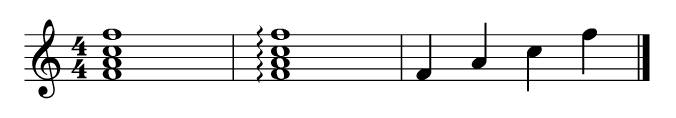
\includegraphics[width=0.8\textwidth]{expanded_major}
\caption{A stable F major chord played out over three time scales, as a true simultaneity, an arpeggiation, and four non-overlapping quarter notes.}
\label{fig:expanded_major}
\end{figure}

\begin{figure}[t]
\centering
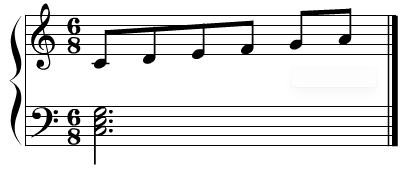
\includegraphics[width=0.6\textwidth]{nonchord_tones}
\caption{A stable C major chord is embellished by passing non-chord tones.}
\label{fig:nonchord_tones}
\end{figure}

% True simultaneity doesn't always make a chord
On the other hand, as shown in Figure \ref{fig:nonchord_tones}, the simultaneous sounding of different notes does not necessarily give rise to the perception of different chords.
Here, a major triad is sustained under the first several degrees of its scale.
While three notes in the upper voice are contained in the C-major triad, the others --the D, F, and A-- are referred to as ``nonchord'' tones.
These extra notes are explained away in the overall harmonic scene, as they fall on metrically weak beats, are comparatively short in duration, and quickly move to notes that \emph{are} in the chord.
These embellishments do not contribute to the harmonic center of the phrase, and the bar can still be understood as a stable C major chord.


\begin{figure}[t]
\centering
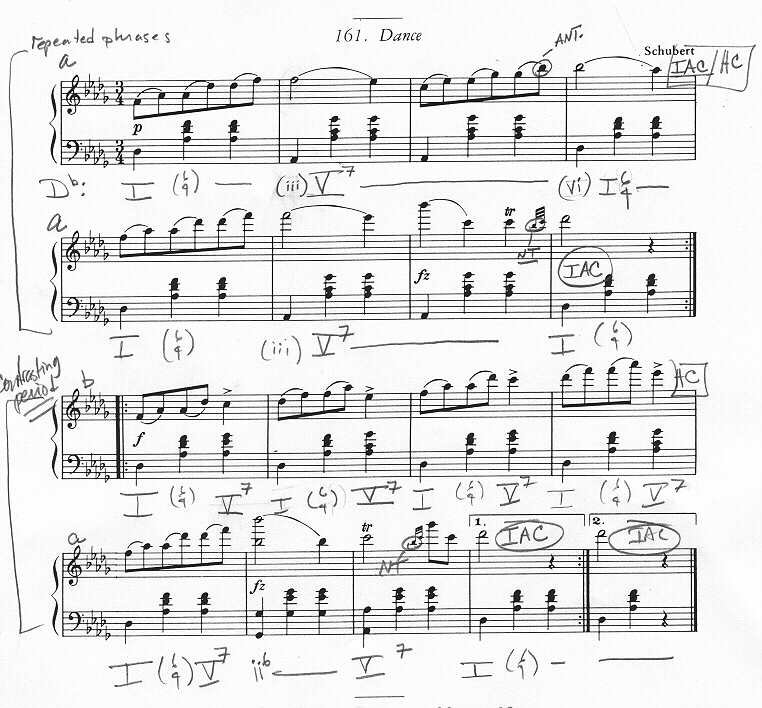
\includegraphics[width=\textwidth]{practicekey2.jpg}
\caption{A sample harmonic analysis of a piano piece, performed as a music theory exercise.}
\label{fig:mthomework}
\end{figure}

A last example, shown in Figure \ref{fig:mthomework}, illustrates the level of complexity and decision making that may arise in the process of describing music in the language of chords.
Referred to as \emph{harmonic analysis}, this exercise is performed in an effort to understand the harmonic content in a theoretical manner, such that chords are notated alongside the original score.
There are many observations one might draw from this example, but a few are of particular interest here.
First, even in an instance such as this, where an individual is able to operate directly on the symbolic representation, it is common to find alternate reasonable interpretations of the same musical content.
As notated in measure 2 for example, the combination of the $A$ and $F$ can be understood both as an embellishment on the $I$, or as an implied $iii$ chord.
When performed, however, the musician can influence how one might perceive this simultaneity through the use of expressive timing or dynamics.
Additionally, this instance focuses on a harmonically simple excerpt for solo piano.
The introduction of other voices will only serve to complicate the resulting musical surface, especially where timbre is considered.
Lastly, this kind of theoretical analysis is developed in, and largely tailored to, the tradition of Western tonal music.
While contemporary popular music is certainly influenced by this tradition, it by no means adheres to the same rules and conventions.


\subsection{Chord Syntax}
\label{sec:chord_syntax}

It is a pragmatic but necessary prerequisite step to define a standard syntax for compactly notating chords.
Much of the pioneering work in this space was performed by Harte \cite{Harte2005Symbolic}, and many of these conventions are utilized here.
Going forward, chords expressed in this scheme are stylized with a fixed-width font, e.g. \texttt{A:min}.

Firstly, Harte's general chord notation is described by the following four-part symbolic description:

\begin{equation}
\texttt{root}:\texttt{quality}~(\texttt{intervals})~/~\texttt{bass}
\end{equation}

\noindent Every chord name begins with a \texttt{root} in the form of a pitch class, optionally modified by zero or more sharps or flats, or one of two reserved characters: \texttt{N} for the ``null'' no-chord condition, or \texttt{X} for the special case in which the musical content cannot be described harmonically.

The root is potentially followed by a \texttt{quality} shorthand, separated by a colon and implying a particular set of note intervals.
Though there are a large number of possible chord qualities, this is often limited to a particular subset.
Those considered in this work are indicated in Table \ref{tab:qualities}.

\begin{table}[t]
\begin{center}
\caption{Chord quality names and corresponding relative semitones.}
\label{tab:qualities}
\begin{tabular}{l | c | c}
Name & Shorthand & Semitones \\
\hline
Major & \texttt{maj} & $\{0, 4, 7\}$ \\
Minor & \texttt{min} & $\{0, 3, 7\}$ \\
Major 7 & \texttt{maj7} & $\{0, 4, 7, 11\}$ \\
Minor 7 & \texttt{min7} & $\{0, 3, 7, 10\}$ \\
Dominant 7 & \texttt{7} & $\{0, 4, 7, 10\}$ \\
Major 6 & \texttt{maj6} & $\{0, 4, 7, 9\}$ \\
Minor 6 & \texttt{min6} & $\{0, 3, 7, 9\}$ \\
Diminished & \texttt{dim} & $\{0, 3, 6\}$ \\
Augmented & \texttt{aug} & $\{0, 4, 8\}$ \\
Suspended 2$^{nd}$ & \texttt{sus2} & $\{0, 2, 7\}$ \\
Suspended 4$^{th}$ & \texttt{sus4} & $\{0, 5, 7\}$ \\
Fully-diminished 7 & \texttt{dim7} & $\{0, 3, 6, 9\}$ \\
Half-diminished 7 & \texttt{hdim7} & $\{0, 3, 6, 10\}$ \\
\hline
\end{tabular}
\end{center}
\end{table}


The third field provides a set of \texttt{intervals}, wrapped by parentheses.
In practice, there are two reasons for representing information intervallically.
One such instance is, through a combination of additional degrees and asterisks, the modification of a quality shorthand in order to represent a non-standard, but related, chord.
An example of this might be the chord name \texttt{A:min($\ast$b3, b7)}, indicating that the minor third ($C$) is absent and a minor 7 ($G$) has been added.
The other instance occurs when the intervals are certain but the quality is ambiguous, such as \texttt{C:(1, 5)}. %; note that this is a valid spelling of the chord shown in Figure \ref{fig:powerchord_context}.

The final field of this chord syntax is the \texttt{bass} interval, which indicates the scale degree of the lowest contributing pitch.
Typically this is also the root of the chord, and is implied as such in the absence of an explicit bass interval.
However, it is necessary to state that the scale degrees of the chord ---given by the quality shorthand and the interval set--- can be further augmented by the inclusion of a bass interval.
For example, the chords \texttt{C:maj/b7} and \texttt{C:7} would be understood as containing the same pitch classes, but are spelled differently.


\subsection{Motivation}
\label{subsec:motivation}

% Historical Context
Even from the earliest efforts in content-based MIR, automatic music transcription has stood as one of the Holy Grails of the field.
Time would prove this to be an exceptionally difficult problem, and fracture this common cause into a variety of smaller, and hopefully more manageable, subtopics.
Automatic chord estimation materialized as one such task, now receiving healthy attention for more than a decade, and is established as a benchmark challenge at the annual MIReX event\footnote{{http://www.music-ir.org/mirex/wiki/MIREX\_HOME}}.

% Applications
% - People
Given the prerequisite skill necessary to produce chord transcriptions manually from recorded audio, there is considerable motivation to develop automated systems capable of reliably performing this task.
As evidenced by large online communities surrounding websites like e-chords\footnote{http://www.e-chords.com} or Ultimate Guitar\footnote{http://www.ultimate-guitar.com}, countless individuals invest considerable time and effort in the curation and consumption of popular music transcriptions.
Often this is driven by desire to learn and perform music for which symbolic notation does not exist.
Conversely, automatic chord estimation systems would be particularly useful in the areas of composition, recording, and production.
Furthermore, the curation of this content would enable large-scale musicological analysis of contemporary music.

% MIR Systems
In addition to the concerns of individual users, computational systems capable of reliable chord estimation are directly useful inside the domain of content-based MIR.
Chords can serve as a robust mid-level representation with which to build systems and extract higher level musical knowledge, and have been used for cover song retrieval \cite{Bello2007Audio} and genre recognition \cite{Anglade2009Genre}.
Such systems would also facilitate data collection for other tasks, aiding in visualization and other facets of music transcription.

% Theoretical merit
From a more philosophical perspective, the identification of chords is also intriguing as an intelligent musical behavior, being a high level cognitive process that is often open to multiple interpretations between knowledgeable experts.
Experiential bias of the annotator may manifest in the subjective decisions made by an observer, where a pianist may arrive at a different harmonic analysis than that of a guitarist due to how a collection of notes might be produced.
Finally, the knowledge and skill of the one recognizing chords in music will affect the resulting interpretations.
Beginners will likely prefer simple or more common descriptions, whereas experts will be more aware of complex nuances and have better command over a larger harmonic vocabulary.


\subsection{Limitations}
\label{subsec:limitations}

% Limitations
It should be acknowledged that this inquiry is subject to the limitations of tonal theory and chords as a language with which to describe a piece of music.
% Scope of music considered
Primarily, this work is interested in the tradition of tonal Western music, with a particular focus on popular contemporary music from the last century, in 12-TET.
% Historical context -> Harmonic analysis
Within this large body of music content, the use of harmony and chords has steadily evolved over time.
Classically, music theorists have long sought to characterize musical works via analysis and reduction as a means to understanding, typically operating from a symbolic representations, i.e. a score.
% As sound recording is a relatively modern invention on the timescale of music history, much more effort to this end has been devoted to the analysis of scores than signals.
% From the counterpoint of J. S. Bach to the functional analysis of Heinrich Schenker or more recently Fred Lehrdal, traditional musical analysis revolves heavily around the harmonic facets of notated music by marginalizing the dimensions of rhythm and timbre.
As a result, the language of ``chords'' developed as an expressive, yet compact, language with which one might describe a piece of music harmonically.
However, Western ``pop music'', infused with elements of folk, blues, jazz, rock and countless other influences, is not to required to adhere to or consider the rules of traditional tonal theory \cite{Tagg1982Analysing}.
Thus efforts to understand the former in the language of the latter is ultimately limited by the validity in doing so.

Even in the constrained space of Western tonal music set forth here, not all musical works will be well-described by the language of harmonic analysis, and thus chords may be a clumsy language with which to describe such music.
An alternative approach to analysis, such as voice leading, might make more sense in this instance;
in others, such as ``math rock'', a lack of clearly structured harmonic content may arguably render the goal of harmonic analysis irrelevant \cite{Cateforis2002Alternative}.
As genre is itself an amorphous and ill-defined concept, the degree to which a piece of music might be understood harmonically will vary, both absolutely and internally.

% Finally, as discussed at the beginning of this document,
% This realization encourages due consideration of the philosophical limits of objective truth in an inherently subjective task.
% As outlined previously, the definition of a chord is open to interpretation, and one's understanding of a harmonic phrase may be influenced by individual experience, degree of skill, and intended purpose.
% Furthermore, the methodology of using ``expert'' annotations in the development and evaluation of computational systems is based on the assumption that all experts share one perspective.


\section{Previous Research in Automatic Chord Estimation}
\label{sec:background}

Building upon the conceptual foundations addressed previously, automatic chord estimation research can be described in three parts.
% Problem Definition
First, an effort is made to formally define the goals of computational systems.
% Previous approaches
The research lineage is then surveyed, identifying commonalities between this work and highlighting the state of the art.
% Data and Evaluation
Approaches to evaluation methodology are discussed last, including a review of data used to benchmark the research presented here.


\subsection{Problem Formulation}
\label{subsec:problem_formulation}

% Problem formulation
Following the motivations outlined in \ref{subsec:motivation}, the goal of an automatic chord estimation (ACE) system is --or, at least, has been-- to produce ``good'' time-aligned sequence of chords from a given music signal.
% This notion of objectivity is crucial to how the problem is approached.
% Critically, two facets of this problem statement require further clarification: one, what is the valid space of chords considered? and two, how might the quality an estimated chord sequence be measured?
% What do we want -- what is meant by chords
As discussed in \ref{sec:chord_syntax}, it is a particular nuance of chord notation that the space of valid spellings is effectively infinite.
To constrain the complexity of the task at hand, ACE systems are traditionally designed to estimate chords from a finite \emph{vocabulary}, defined \emph{a priori}.
This simplification reduces the chord estimation to a classification problem, where all observations are assigned to one of $K$ chord \emph{classes}.

%  While the majority of musical content will be described by a small subset of chords, a large number of infrequently occurring chord names will arise naturally in a collection of real music.
% This imbalance is amplified by the reality that some chord qualities, namely \texttt{maj} or \texttt{min}, simply occur more often in Western music.
Historically, the choice of chord vocabulary has been anything but standard, influenced primarily by the data available to a researcher.
Supervised machine learning approaches, for example, can be sensitive to the amount of labeled data available for training, in which case it might be advantageous to only consider sufficiently represented chord classes.
Furthermore, not all researchers have access to the same data, introducing another degree of variability.
As a result, it can be challenging, if not impossible, to compare the performance of systems designed for different chord vocabularies.

To address this challenge, one common strategy employed by the research community is that of Major-Minor chord resolution.
Based on the common 24 Major and minor keys, this formulation proceeds by mapping all chords in a collection to either a Major or Minor chord with the same root \cite{McVicar2013Machine}.
While this results in some musically reasonable chord mappings, e.g. \texttt{maj7} $\to$ \texttt{maj}, others are more difficult to justify, e.g. \texttt{dim7} $\to$ \texttt{min} or \texttt{aug} $\to$ \texttt{maj}.

Having framed chord estimation as a classification problem, there are two critical assumptions to note going forward.
First, the classification paradigm operates on the notion that the relationship between an observation and its corresponding class is stable.
Chord estimation research has classically leveraged expert musicians in the spirit of achieving objectivity, but this is ultimately an approximation to some unknown degree.
Second, flat classification problems ---those in which different classes are conceptually independent--- are built on the assumption of mutually exclusive relationships.
In other words, assignment to one class precludes the valid assignment to any other classes considered.
For example, ``cat'' and ``dog'' are mutually exclusive classes of ``animal'', but ``cat'' and ``mammal'' are not.
Returning to chords, \texttt{C:dim7} and \texttt{C:maj} are clearly mutually exclusive classes, but it is difficult to say the same of \texttt{C:maj7} and \texttt{C:maj}, as the former \emph{contains} the latter.


\subsection{Computational Approaches}
\label{subsec:computational_approaches}

\begin{figure}[t]
\centering

\includegraphics[width=0.8\textwidth]{TODO}
\caption{Block-diagram of the common building blocks in modern automatic chord estimation systems.}
\label{fig:basic_ace}
\end{figure}

% Previous work
Considering the space of ACE research, nearly all approaches to the task adopt the same basic architecture, diagrammed in Figure \ref{fig:basic_ace}.
First, harmonic features, referred to as pitch class profiles (PCP) or \emph{chroma}, are extracted from short-time observations of the audio signal.
Initially proposed for use in chord estimation systems by Fujishima \cite{Fujishima1999Realtime}, chroma features attempt to measure the amount of energy in the signal corresponding to the 12 pitch classes named in Eq. \ref{eq:pitch_classes}.
These features may then be processed by any number of means, referred to in the literature as \emph{pre-filtering}.
Importantly, this is done prior to the next stage of \emph{pattern matching}, which is performed on the final feature representation to measure how similar the observed signal is to a set of chord names.
The process of pattern matching, a relatively local operation, is mapped over a much longer signal, e.g. a full recording, yielding a time-varying estimate of the various chord types the model can represent.
Finally, \emph{post-filtering} is applied to the output of the pattern matching stage, resulting in a sequence of chord names over time.

Though the implementation details have continued to evolve over the last decade, the brunt of chord estimation research has concentrated not on the fundamental system per se, but rather the tuning of its components.
In particular, much time and energy has been invested in developing not just better features, but specifically better \emph{chroma} features \cite{Mueller2010Towards}.
Complementing chroma features, others have explored the use of multi-band chroma to model bass frequencies separately \cite{Mauch2010Simultaneous} or a Tonnetz representation in an effort to better encode harmonic relationships between chords \cite{Lee2007Unified}.
Acknowledging the challenges inherent to designing good features, Pachet et al pioneered work in automatic feature optimization \cite{Pachet2006Recognizing}, and more recently deep learning methods have been employed to learn robust Tonnetz features \cite{Humphrey2012Learning}.
Early methods focused on local smoothing, such as low-pass or median filtering as a form of pre-filtering \cite{Cho2010Exploring}, but more recently some methods have attempted to leverage the repeated nature of music to yield more stable estimates of the harmonic composition at a given point in time \cite{Cho2011Feature}.
Various classification strategies have been investigated such as binary templates \cite{Oudre2009Template}, Dirichlet distribution models \cite{Burgoyne2005Learning}, or Support Vector Machines (SVMs) \cite{Weller2009Structured}, but Gaussian Mixture Models (GMM) are by and large the most common feature modeling approach \cite{Cho2014Improved}.
The choice of post-filtering methods has been shown to significantly impact system performance, and much research has focused on properly tuning Hidden Markov Models (HMMs) \cite{Cho2010Exploring}, first introduced by \cite{Sheh2003Chord}.
Recently, in an effort to continue to advance the state of the art, researchers have begun exploring more complex post-filtering methods such as Dynamic Bayesian Networks (DBNs) \cite{Mauch2010Approximate}, Conditional Random Fields \cite{Sumi2012Music}, and Variable-Length Markov Models \cite{Chordia2011Predictive}.

It is worth noting that in this lineage, the systems that do make use of data-driven learning typically only do so in disjoint stages.
More often than not, machine learning is only performed at the pattern matching stage, where increasingly powerful models are fit to hand-crafted features.
A few works do attempt to learn features, such as \cite{Mauch2010Approximate, Humphrey2012Learning}, but the different stages are optimized independently.
Though it is standard practice to train a GMM/HMM jointly, some have observed that learning the parameters of the HMM, i.e. the transition probabilities, yields no significant benefit over a uniform probabilities with a strong self-transition affinity \cite{Cho2014Improved}.
One notable work that attempts to jointly optimize multiple stages is that of \cite{Cho2012Minimum}, which optimizes the GMM to a minimum frame classification error, rather than a conventional maximum likelihood formulation.


\subsection{Evaluation Methodology}
\label{subsec:eval_methodology}

In order to objectively measure the quality of a proposed ACE system, it is necessary to address two related components: the collection of ground-truth data, and the manner in which estimations are compared to this reference data.

The first major effort to curate ground truth chord transcriptions was led by Harte in the mid-2000s, referred to as the Isophonics dataset\footnote{\url{http://isophonics.net/content/reference-annotations}}, where a small team of researchers transcribed the entire discography of The Beatles.
Containing chord annotations for 180 tracks, this was a landmark dataset in the field of MIR and shaped years of ACE research.
Importantly, this transcription effort leveraged professional transcriptions of the music under consideration, and was verified for accuracy multiple times.
However, despite this rigor, the data is drawn from a single artist and very well known to the research community; some have argued that ACE research has begun to manually overfit this collection.

To combat these issues, two datasets were released following the 2011 Conference of the International Society of Music Information Retrieval (ISMIR), one of over 700 tracks led by J. Ashley Burgoyne \cite{Burgoyne2011Expert} and another of 295 tracks led by Tae Min Cho, from the Music and Audio Research Lab at NYU\footnote{\url{https://github.com/tmc323/Chord-Annotations}}; here, the former is referred to as ``Billboard'' and the latter as ``MARL-Chords'', corresponding to their related projects.
In parallel, an additional, comparatively small, dataset was released, containing 20 tracks by the band Queen, provided by Matthias Mauch as an extension to the Isophonics set.
In all four cases, the chord transcriptions are provided as ``ground truth'', on the premise that the data corresponds to the expert perspective.
To help prevent errors and resolve judgment calls, these additional annotation efforts employed a review process, where the transcriptions of one or more annotators were verified by a different individual.

Leveraging this ground truth data, it is possible to quantitatively assess the outputs of a computational system.
% The approach to comparing, and subsequently scoring, the relative agreement between two chord transcriptions can be formally expressed .
Expressed formally, the conventional approach to scoring an ACE system is a weighted measure of chord-symbol recall, $R_{W}$, between a reference, $\mathcal{R}$, and estimation, $\mathcal{E}$, chord sequence as a \emph{continuous} integral over time, summed over a collection of $N$ pairs:

\begin{equation}
\label{eq:recall_micro}
R_{W} = \frac{1}{S}\sum_{n=0}^{N-1}\int_{t=0}^{T_n}C(\mathcal{R}_n(t), \mathcal{E}_n(t))~dt
\end{equation}

\noindent Here, $C$ is a chord \emph{comparison} function, bounded on $[0, 1]$, $t$ is time, $n$ the index of the track in a collection, $T_n$ the duration of the $n^{th}$ track. $S$ corresponds to the cumulative amount of time, or \emph{support}, on which $C$ is defined, computed by a similar integral:

\begin{equation}
S = \sum_{n=0}^{N-1}\int_{t=0}^{T_n}(\mathcal{R}_n(t), \mathcal{E}_n(t) \in \Re)~dt
\end{equation}

Defining the normalization term $S$ separately is useful when comparing chord names, as it relaxes the assumption that the comparison function is defined for all possible chords.
Furthermore, setting the comparison function as a free variable allows for flexible evaluation of a system's outputs, and thus all emphasis can be placed on the choice of comparison function, $C$.
In practice, this measure has been referred to as \emph{Weighted Chord Symbol Recall} (WCSR) \cite{Harte2010Towards}, \emph{Relative Correct Overlap} (TCO) \cite{McVicar2013Machine}, or \emph{Framewise Recognition Rate} \cite{Cho2014Improved}, but it is, most generally, a recall measure.

As discussed, most ACE research typically proceeds by mapping all chords into a smaller chord vocabulary, and using an enharmonic equivalence comparison function at evaluation, e.g. \texttt{C\#:maj} == \texttt{Db:maj}.
Recently, this approach was generalized by the effort behind the open source evaluation toolbox, \texttt{mir\_eval} \cite{Raffel2014Eval}, introducing a suite of chord comparison functions.
The seven rules considered here are summarized in Table \ref{tab:mir_eval}.

\begin{table}[t]
\begin{center}
\caption{Chord comparison functions and examples in \texttt{mir\_eval}.}
\label{tab:mir_eval}
\begin{tabular}{l | c | c | c }
Name & Equal & Inequal & Ignored \\
\hline
Root & \texttt{G\#:aug}, \texttt{Ab:min} & \texttt{C:maj/5}, \texttt{G:maj} & -- \\
Thirds & \texttt{A:maj}, \texttt{A:aug} & \texttt{C:maj7}, \texttt{C:min} & --\\
Triads & \texttt{D:dim}, \texttt{D:hdim7} & \texttt{D:maj}, \texttt{D:aug} & -- \\
Sevenths & \texttt{B:9}, \texttt{B:7} & \texttt{B:maj7}, \texttt{B:7} & \texttt{sus2}, \texttt{dim} \\
Tetrads & \texttt{F:min7}, \texttt{F:min(b7)} & \texttt{F:dim7}, \texttt{F:hdim7} & -- \\
majmin & \texttt{E:maj}, \texttt{E:maj7} & \texttt{E:maj}, \texttt{E:sus2} & \texttt{sus2}, \texttt{dim} \\
MIREX & \texttt{C:maj6}, \texttt{A:min7} & \texttt{C:maj}, \texttt{A:min} \\
\hline
\end{tabular}
\end{center}
\end{table}

The meaning of most rules may be clear from the table, but it is useful to describe each individually.
The ``root'' comparison only considers the enharmonic root of a chord spelling.
Comparison at ``thirds'' is based on the minor third scale degree, and is equivalent to the conventional mapping of all chords to their closest major-minor equivalent.
In other words, a chord with a minor-third is minor, e.g. $\texttt{dim7} \to \texttt{min}$, and \emph{all} other chords map to major, e.g. $\texttt{sus2} \to \texttt{maj}$.
The ``triads'' rule considers the first seven semitones of a chord spelling, encompassing the space of major, minor, augmented, and diminished chords.
The ``sevenths'' rule is limited to major-minor chords and their tetrad extensions, i.e. major, minor, and dominants;
chords outside this set are considered ``out-of-gamut'' and ignored.
The ``tetrads'' comparison extends this to all chords contained within an octave, e.g. six chords and half-diminished sevenths.
The ``Major-minor'' comparison is limited to major and minor chords alone;
like ``sevenths'', other chords are ignored from evaluation.
Unlike the other rules, ``MIREX'' compares chords at the pitch class level, and defines equivalence if three or four notes intersect.
Comparing the pitch class composition of a chord allows for a slightly relaxed evaluation, allowing for misidentified roots and related chords.
Finally, rules that ignore certain chords only do so when they occur in a reference annotation.
In other words, an estimation is not held accountable for chords deemed to be out of gamut, but predicting such chords is still counted as an error.

Complementing these rules, it was recently proposed by Cho in \cite{Cho2014Improved} that, when working with larger chord vocabularies, special attention should be paid to performance across all chord qualities.
The motivation for additional measures stems from the reality that chord classes are not uniformly distributed, and a model that ignores infrequent chords will not be well characterized by global statistics.
Instead, Cho proposes a chord quality recall measure, $R_{Q}$ whereby all chord comparisons are rotated to their equivalents in C, and averaged without normalizing by occurrence.

\begin{equation}
R_{Q} = \sum_{q=0}^{Q-1}\frac{1}{W_q}\sum_{n=0}^{N-1}\int_{t=0}^{T_n}C(\mathcal{R}_n(t), \mathcal{E}_n(t) | q)\partial~t
\end{equation}

\noindent Referred to originally as \emph{Average Chord Quality Accuracy} (ACQA), this metric weights the contributions of the individual chord qualities equally, regardless of distribution effects.
Notably, as the overall chord distribution becomes more uniform, this measure will converge to Eq. (\ref{eq:recall_micro}).
However, given the significant imbalance of chord classes, large swings in any overall weighted recall statistic may result in small differences of the quality-wise recall, and vice versa.
It should also be noted that the only comparison function on which quality-wise recall is well defined is strict equivalence.


\section{Pilot Study}
\label{sec:pilot_study}

Here, a preliminary study conducted by the author in 2012, and presented at the International Conference of Machine Learning and Applications (ICMLA 2012), is revisited and expanded upon to frame subsequent work \cite{Humphrey2012Rethinking}.
Approaching ACE from the perspective of classifying music audio among the standard 24 Major-Minor classes, in addition to a no-chord estimator, a deep convolutional network is explored as a means to realize a full chord estimation system.
Doing so not only addresses the questions of relevance or quality toward chroma as a representation, but error analysis of an end-to-end data-driven approach can be used to gain insight into the data itself.
% Even in the instances of previous work that jointly optimize different processing stages, these systems are limited by the choice of hand-crafted features, e.g. chroma.
% Though the notion of feature optimization is an open question, history indicates most believe more powerful classifiers will lead to better results.
% It has been adequately demonstrated in other disciplines that deep learning can be used to train feature extractors and a classifier jointly, resolving this issue.
% Additionally, this approach makes it easy to build overly complex models, at which point it can be trivial to overfit the data used for training.
% Though often thought a deficiency, it is seen here as a opportunity to better understand the problem,
This observation gives rise to two related questions: one, how does performance change as a function of model complexity, and two, in what instances can the model \emph{not} overfit the training data?
% Furthermore, how can domain knowledge be used to inform the application of a deep learning to the estimation of chords from audio?


\subsection{Experimental Setup}
\label{subsec:experimental_setup}

% Input Representations
Audio signals are downsampled to 7040Hz and transformed to a constant-Q time-frequency representation.
This transform consists of 36 bins per octave, resulting in 252 filters spanning 27.5--1760Hz, and is applied at a framerate of 40Hz.
The high time-resolution of the constant-Q spectra is further reduced to a framerate of 4Hz by mean-filtering each frequency coefficient with a 15-point window and decimating in time by a factor of 10.
As discussed previously, a constant-Q filterbank front-end provides the dual benefits of a reduced input dimensionality, compared to the raw audio signal, and produces a time-frequency representation that is linear in pitch, allowing for convolutions to learn pitch-invariant features.

The input to the network is defined as a 20-frame time-frequency \emph{patch}, corresponding to 5 seconds.
A long input duration is chosen in an effort to learn context, thereby reducing the need for post-filtering.
Local-contrast normalization is applied to the constant-Q representation, serving as a form of automatic gain control, and somewhat similar in principle to log-whitening used previously in chord estimation \cite{Cho2010Exploring}.
As an experimental variable, data are augmented by applying random circular shifts along the frequency axis during training within an octave range.
The linearity of pitch in a constant-Q representation affords the ability to ``transpose'' an observation as if it were a chord of a different root by shifting the pitch tile and changing the label accordingly.
Every data point in the training set then contributes to each chord class of the same quality (Major or minor), having the effect of inflating the dataset by a factor of 12.
The two conditions ---before and after augmentation--- are referred to henceforth as ``As-Is'' and ``Transposed''.

% Architectures
A five-layer 3D convolutional network is used as the general model, consisting of three convolutional layers and two fully-connected layers. % ; a diagram is provided in Figure \ref{fig:chordnet_take1}.
Six different model complexities are explored by considering two high-level variables, given in Table \ref{tab:model_configs}.
The width of each layer, as the number of kernels or units, increases over a small (S), medium (M), and large (L) configuration.
Two different kernel shapes are considered, referred to as $1$ and $2$.
Note that only the first convolutional layer makes use of pooling, and only in the frequency dimension, by a factor of three in an effort to learn slight tuning invariance.
The output of the final layer is passed through a softmax operator, producing an output that behaves as a likelihood function over the chord classes.


\begin{table}[!t]
% increase table row spacing, adjust to taste
\renewcommand{\arraystretch}{1.4}
\caption{Model Configurations - Larger models proceed down the rows, as small (S), medium (M), and large (L); two different kernel shapes, $1$ and $2$, are given across columns.}
%\caption{Convolutional Layers -- K: kernel shape, P: pooling shape. Fully-connected Layers -- W: Weight shape }
\label{tab:model_configs}
\centering
\begin{tabular}{c || l || l |}
 & 1 & 2 \\
\hline
 S & K:(1, 4, 6, 25), P:(1, 3)& K:(1, 4, 5, 25), P:(1, 3)\\
 &K:(4, 6, 6, 27) & K:(4, 6, 5, 13) \\
 &K:(6, 8, 6, 27) & K:(6, 8, 5, 13) \\
 &W:(480, 50)  & W:(2560, 50)\\
 &W:(50, 25)  & W:(50, 25)\\
\hline
 M & K:(1, 6, 6, 25), P:(1, 3)& K:(1, 6, 5, 25), P:(1, 3)\\
 &K:(6, 9, 6, 27) & K:(6, 9, 5, 13) \\
 &K:(9, 12, 6, 27) & K:(9, 12, 5, 13) \\
 &W:(720, 125)  & W:(3840, 125)\\
 &W:(125, 25)  & W:(125, 25)\\
\hline
 L & K:(1, 16, 6, 25), P:(1, 3)& K:(1, 16, 5, 25), P:(1, 3)\\
 &K:(16, 20, 6, 27) & K:(16, 20, 5, 13) \\
 &K:(20, 24, 6, 27) & K:(20, 24, 5, 13) \\
 &W:(1440, 200)  & W:(7680, 200)\\
 &W:(200, 25)  & W:(200, 25)\\
\hline
\end{tabular}
\end{table}


% Training
As this work predates access to the Billboard and Queen datasets, only the MARL-Chords and Beatles collections are considered, totaling 475 tracks.
All chords are resolved to their nearest major-minor equivalent, as discussed in Section \ref{subsec:problem_formulation}, based on the third scale degree: \texttt{min} if the quality should contain a flat third, otherwise \texttt{maj}.
The collection of 475 tracks are stratified into five folds, with the data being split into training, validation, and test sets at a ratio of 3--1--1, respectively.
The algorithm by which the data are stratified is non-trivial, but somewhat irrelevant to the discussion here; the curious reader is referred to the original publication for more detail.
Model parameters are learned by minimizing the Negative Log-Likelihood (NLL) loss over the training set.
This is achieved via mini-batch stochastic gradient descent with a fixed learning rate and batch size, and early stopping is performed as a function of classification error over the validation set.
Training batches are assembled by a forced uniform sampling over the data, such that each class occurs with equal probability.

\subsection{Quantitative Results}
\label{subsec:quantitative_results}

Following the discussion of evaluation in \ref{subsec:eval_methodology}, the only comparison function used here is ``thirds'', and all statistics correspond to a weighted recall measure.

\begin{table}[!t]
% increase table row spacing, adjust to taste
% \renewcommand{\arraystretch}{1.4}
% if using array.sty, it might be a good idea to tweak the value of
% \extrarowheight as needed to properly center the text within the cells
\caption{Overall recall for two models, with transposition and LCN.}
\label{tab:exp1res}
\centering
% Some packages, such as MDW tools, offer better commands for making tables
% than the plain LaTeX2e tabular which is used here.
\begin{tabular}{c || c c c || c c c |}
 & \multicolumn{3}{| c ||}{L-1} & \multicolumn{3}{c|}{S-1} \\
 \hline
Fold & Train & Valid & Test & Train & Valid & Test \\
\hline
1 & 83.2 & 77.6 & 77.8 &  79.6 & 76.9 & 76.8 \\
2 & 83.6 & 78.2 & 76.9 & 80.5 & 77.0 & 76.8 \\
3 & 82.0 & 78.1 & 78.3 & 80.0 & 77.2 & 78.2\\
4 & 83.6 & 78.6 & 76.8 & 80.2 & 78.0 & 75.8 \\
5 & 81.7 & 76.5 & 77.7 & 79.5 & 75.9 & 76.8 \\
\hline
Total &  82.81 & 77.80 & \textbf{77.48} & 79.97 & 77.00 & \textbf{76.87}\\
\hline
\end{tabular}
\end{table}

As an initial benchmark, it is necessary to consider performance variance over different test sets.
The outer model configurations in the first column of Table \ref{tab:model_configs} (Arch:L-1 and Arch:S-1) were selected for five-fold evaluation, influenced by run-time considerations.
Overall recall is given in Table \ref{tab:exp1res}, and offers two important insights.
One, deep network chord estimation performs competitively with the state of the art at the major-minor task.
Previously published numbers on the same dataset fall in the upper 70\% range \cite{Cho2010Exploring}, and it is encouraging that this initial inquiry roughly matches state of the art performance.
Noting the variation in performance falls within a 2\% margin across folds, a leave-one-out (LoO) strategy is used for experimentation across configurations, with and without data transposition.

The overall recall results are given in Table \ref{tab:exp2res}.
Perhaps the most obvious trend is the drop in recall on the training set between data conditions.
Transposing the training data also improves generalization, as well as reducing the extent to which the network can overfit the training data.
Transposing the input pitch spectra should have a negligible effect on the parameters of the convolutional layers, and this is confirmed by the results.
All models in the second column, e.g. X-2, have smaller kernels, which leads to a much larger weight matrix in the first fully connected layer, and worse generalization in the non-transposed condition.
It is reasonable to conclude that over-fitting mostly occurs in the final layers of the network, which do not take advantage of weight tying.
Transposing the data results in an effect similar to that of weight tying, but because the sharing is not explicit the model must learn to encode this redundant information with more training data.


\begin{table}[!t]
% increase table row spacing, adjust to taste
% \renewcommand{\arraystretch}{1.4}
% if using array.sty, it might be a good idea to tweak the value of
% \extrarowheight as needed to properly center the text within the cells
\caption{Performance as a function of model complexity, over a single fold.}
\label{tab:exp2res}
\centering
\begin{tabular}{ c || c c c || c c c |}
& \multicolumn{3}{c||}{As-Is} & \multicolumn{3}{|c|}{Transposed}\\
 \hline
Arch & Train & Valid & Test & Train & Valid & Test \\
\hline
S-1 & 84.7 & 74.9 & 75.6 & 79.5 & 75.9 & 76.8 \\
M-1 & 85.5 & 75.0 & 75.5 & 80.6 & 75.6 & 77.0 \\
L-1 & 92.0 & 75.2 & 75.5 & 81.7 & 76.5 & 77.7 \\
\hline
S-2 & 87.0 & 73.1 & 74.5 & 78.4 & 75.5 & 76.2 \\
M-2 & 91.2 & 73.9 & 74.0 & 79.4 & 75.4 & 76.6 \\
L-2 & 91.7 & 73.6 & 73.8 & 81.6 & 76.3 & 77.4 \\
\hline
\end{tabular}
\end{table}


\subsection{Qualitative Analysis}
\label{subsec:Qualitative_analysis}

Having obtained promising quantitative results, the larger research objectives can now be addressed.
As indicated by Table \ref{tab:exp2res}, transposing the data during training slightly improves generalization, but does more to limit the degree to which the models can overfit the training data.
These two behaviors are not necessarily equivalent, and therefore whatever these networks learn as a result of data augmentation is preventing it from overfitting a considerable portion of the training set.

\begin{figure}[!t]
\centering
 \centerline{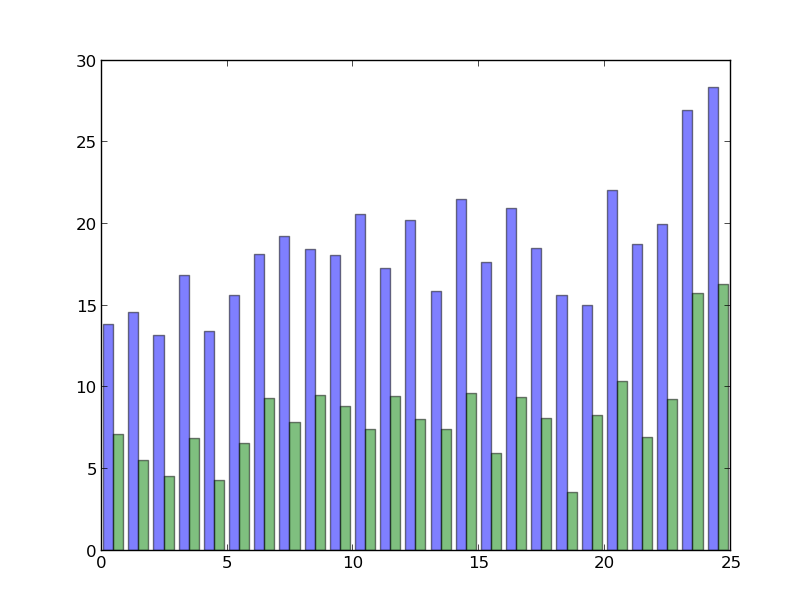
\includegraphics[width=0.8\textwidth]{tr-te-diff_FF-TT}}
\caption{Accuracy differential between training and test as a function of chord class, ordered along the x-axis from most to least common in the dataset for As-Is (blue) and Transposed (green) conditions.}
\label{fig:classes}
\end{figure}

One potential cause of over-fitting is due to an under-representation of some chord classes in the dataset.
If this were the case, the most frequent classes should be unaffected by data augmentation, while less common classes would exhibit drastic swings in performance.
Focusing here on Arch:L-1, Figure \ref{fig:classes} shows the change in accuracy between data conditions for both training and test sets as a function of chord class, sorted by most to least common in the dataset.
This plot indicates that, while transposing data during training reduces over-fitting, it does so uniformly across chord classes, on the order of about $10\%$.
Therefore, all chord classes benefit equally from data augmentation, which is characteristic of intra-class variance more so than inadequate data for less common classes.

\begin{figure}[!t]
\centering
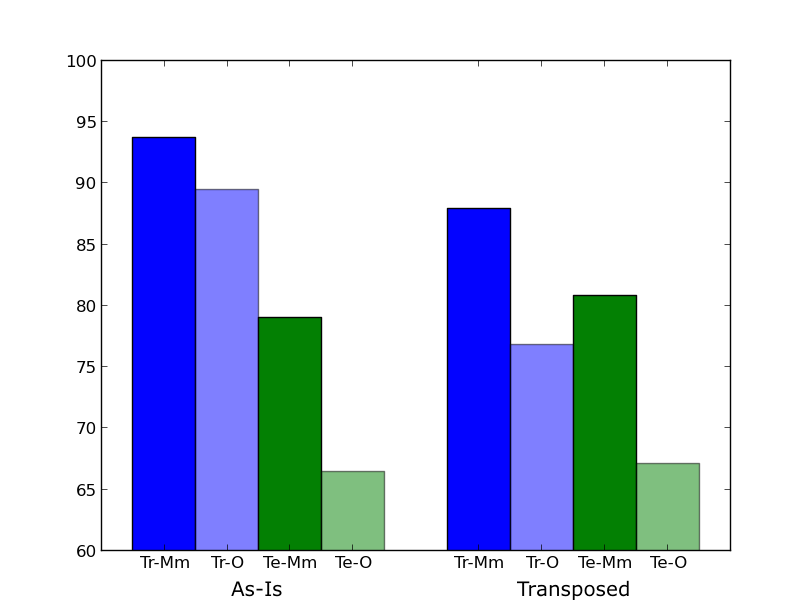
\includegraphics[width=0.8\textwidth]{FF-TT_Mm-vs-other}
\caption{Effects of transposition on classification accuracy as a function explicitly labeled Major-Minor chords (dark bars), versus other chord types (lighter bars) that have been resolved to their nearest Major-Minor equivalent, for training (blue) and test (green) in As-Is (left) and Transposed (right) conditions.}
\label{fig:strict_vs_others}
\end{figure}

If this is indeed the case, there are likely two main sources of intra-class variance: the practice of resolving all chord classes to Major-Minor, or error in the ground truth transcriptions.
As a means to assess the former, Figure \ref{fig:strict_vs_others} plots the accuracy for chords that strictly labeled root-position Major-minor (Mm) versus all other (O) chords that are mapped into these classes in the train (Tr) and test (Te) conditions, with and without transposition.
This is a far more informative figure, resulting in a few valuable insights.
First, there is a moderate drop in performance over the training set for strictly Major-minor chords when data are transposed ($\approx -5\%$), but this causes a noticeable increase in generalization for strictly Major-minor chords in test set ($\approx +3\%$).
Other chords, however, experience a significant decrease in performance within the training set ($\approx -11\%$) with transposition, but register a negligible improvement in the test set ($>1\%$).
One interpretation of this behavior is there is too much conceptual variation in the space of Other chords to meaningfully generalize to unseen data that is also not strictly Major-minor.
This definition by exclusion gives rise to a class subset that is less populated than its strict counterpart, but will inherently contain a wider range of musical content.
Though a sufficiently complex model may be able to overfit these datapoints in the absence of transposition, counting each observation toward every pitch class distributes the added variance across all classes evenly.
This causes the model to ignore uncommon modes in the class distribution as noise, while reinforcing the strict Major-minor model in the process.

\begin{figure}[!t]
\centering
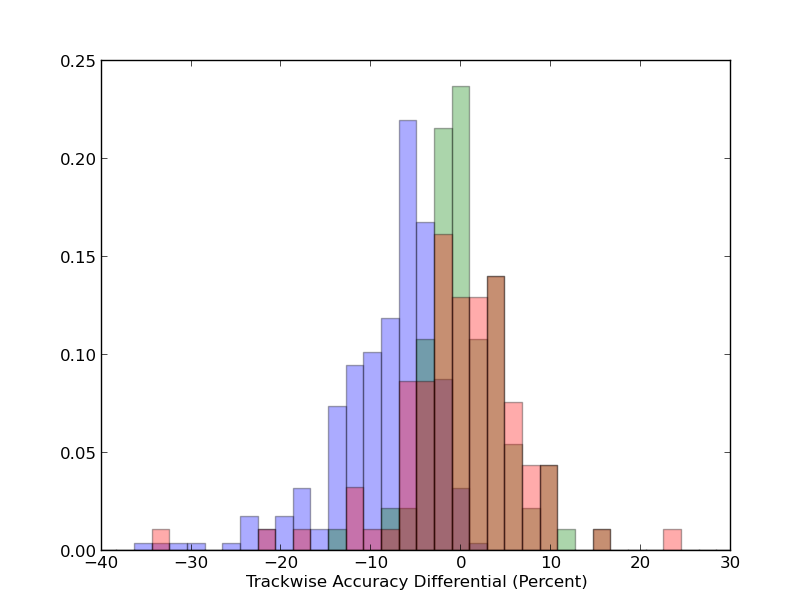
\includegraphics[width=0.8\textwidth]{arch_5-FF_TT_accdiff2}
\caption{Histograms of track-wise recall differential between As-Is and Transposed data conditions, for training (blue), validation (red) and test (green) datasets.}
\label{fig:acc_diff}
\end{figure}

In addition to the effects of vocabulary resolution, there is also the consideration as to where estimation errors reside in the data.
Due to the naturally repetitive nature of music, it is expected that problematic chords will often come from the same track.
More importantly, it is because of this strong internal structure that these chords are likely problematic for similar reasons, and in a manner that might not reveal itself when viewed independently.
Therefore, tracks in the training set that exhibit significantly different performance between data conditions may help answer another question: why might transposition prevent the model from overfitting certain chords?
To investigate this behavior, track-wise histograms of recall differential are computed with and without data transposition for the training, validation, and test splits, shown in Figure \ref{fig:acc_diff}.
Interestingly, performance over most tracks is unaffected or only slightly changed by the transposed data condition, as evidenced by the near-zero mode of the distributions.
Some tracks in the training set, however, yield considerably worse results when the data is transposed.
While this is consistent with intuition, %intuitively satisfying because the repetitive nature of music would cause observations drawn from the same recording to be highly correlated, and therefore multiple instances of rare chords, outliers, or labeling errors should be well localized.
, it indicates that error analysis is sufficiently motivated at the track, rather than instance, level, and may offer insight into future areas of improvement.

One such problem track is ``With or Without You'' by U2.
Here, the ground truth transcription consists primarily of four chords: \texttt{D:maj}, \texttt{D:maj/5}, \texttt{D:maj6/6}, and \texttt{D:maj(4)/4}.
When resolved to the Major-minor vocabulary, the transcription is reduced entirely to \texttt{D:maj}.
In the As-Is data condition, the model is able to call nearly the entire track \texttt{D:maj};
when training data are transposed, however, the model is unable to reproduce the ground truth transcription and instead tracks the bass motion, producing \texttt{D:maj}, \texttt{A:maj}, \texttt{B:min}, and \texttt{G:maj}, a very common harmonic progression in popular music.
As far as quantitative evaluation is concerned, this second estimation exhibits a high degree of mismatch with the reference transcription, but is qualitatively reasonable and arguably far more useful to a musician.
Importantly, this illustrates that the process of mapping chords to a reduced vocabulary can cause objective measures to deviate considerably from subjective experience, and thus confounding evaluation.

However, perhaps even more critically, the reliability of the reference annotation is somewhat dubious.
Returning to the original song, one finds reasonably ambiguous harmonic content, consisting of a vocal melody, the moving bass line mentioned previously, a string pad sustaining a high-pitched \texttt{D}, and a moving guitar riff.
Therefore, as a point of comparison, an Internet search yields six guitar chord transcriptions from the website Ultimate Guitar\footnote{\url{http://tabs.ultimate-guitar.com/u/u2/with_or_without_you_crd.htm},  accessed 19 April 2015.}.
These alternative interpretations are consolidated in Table \ref{tab:wowu_chords}, alongside the reference, noting both the average and number of ratings, as well as the number of views the tab has received.
Though the view count is not directly indicative of a transcription's accuracy, it does provide a weak signal indicating that a large number of users did \emph{not} rate it negatively.
In considering this particular example, there are a handful of takeaways to note.
First, all but the sixth of the user-generated chord transcriptions are equivalent by the conventional major-minor mapping rules, which is, interestingly enough, the same one produced by the model presented here.
Second, this rather large community of musicians shows, at least for this song, a strong preference for root position chords.
While it is difficult to determine why an annotator might choose one interpretation than another, it would appear general, root-position chords are preferred to nuanced chord spellings, e.g. \texttt{G:maj} over \texttt{D:maj(4)/4}.
Finally, this raises questions surrounding the practice of using such precise chord labels for annotation.
If nothing else, the flexibility afforded by this particular chord syntax allows annotators to effectively ``build'' their own chords through non-standard intervals or various bass intervals, amplifying the role subjectivity can play in transcription.
This is not only problematic from a practical standpoint ---are various annotators using this syntax consistently?--- but atypical chord spellings are most likely to appear when the music content being described is especially ambiguous.


\begin{table}[!t]
% increase table row spacing, adjust to taste
% \renewcommand{\arraystretch}{1.4}
% if using array.sty, it might be a good idea to tweak the value of
% \extrarowheight as needed to properly center the text within the cells
\small
\caption{Various real chord transcriptions for ``With or Without You'' by U2, comparing the reference annotation with six interpretations from a popular guitar tablature website; a raised asterisk indicates the transcription is given relative to a capo, and transposed to the actual key here.}
\label{tab:wowu_chords}
\centering
\begin{tabular}{ c || c c c c | c c c c |}
Ver. & \multicolumn{4}{c}{Chord Sequence} & Score & Ratings & Views \\
 \hline
Ref. & \texttt{D:maj} & \texttt{D:maj/5} & \texttt{D:maj6/6} & \texttt{D:maj(4)/4} & --- & --- & --- \\
\hline
1 & \texttt{D:maj} & \texttt{A:maj} & \texttt{B:min} & \texttt{G:maj} & 4/5 & 193 & 1,985,878 \\
2 & \texttt{D:5} & \texttt{A:sus4} & \texttt{B:min7} & \texttt{G:maj} & 5/5 & 11 & 184,611 \\
$3^*$ & \texttt{D:maj} & \texttt{A:maj} & \texttt{B:min} & \texttt{G:maj} & 4/5 & 23 & 188,152 \\
$4^*$ & \texttt{D:maj} & \texttt{A:maj} & \texttt{B:min} & \texttt{G:maj7} & 4/5 & 14 & 84,825 \\
$5^*$ & \texttt{D:maj} & \texttt{A:maj} & \texttt{B:min} & \texttt{G:maj} & 5/5 & 248 & 338,222 \\
6 & \texttt{D:5} & \texttt{A:5} & \texttt{D:5/B} & \texttt{G:5} & 5/5 & 5 & 16,208 \\
\hline
\end{tabular}
\end{table}


\subsection{Conclusions}
\label{subsec:conclusions}

Following this initial inquiry, there are a few important conclusions to draw that should influence subsequent work.
First and foremost, the common practice of major-minor chord resolution is responsible for a significant amount of error, both in training and test.
While this approach simplifies the problem being addressed, it appears to introduce uninformative variation to classes during training, and thus noise in the resulting evaluation.
Therefore, for this reason alone, future work should consider larger vocabulary chord estimation, so that each chord class can be modeled explicitly.
Additionally, an investigation into sources of error revealed that the performance for some tracks changes drastically between data conditions.
Further exploration encouraged the notion that chord annotations with modified intervals or bass information may amplify the subjectivity of a transcription, and thus introduce noise in the reference chord annotations.
Ignoring over-specified chord names would serve as an approach to data cleaning, maximizing confidence in the ground truth data and resulting in more stable evaluation.
% Finally, invariance to absolute pitch height should be built directly into the chord model, eliminating the need to manually transpose data during training.


\section{Large Vocabulary Chord Estimation}
\label{subsec:large_vocabulary_ace}

Combining observations resulting from the previous study with other recent trends in ACE research, the focus now turns to the task of large vocabulary ACE.
There is a small body of research pertaining to vocabularies beyond the major-minor formulation, exploring different mixtures of chord classes and inversions \cite{Mauch2010Simultaneous, Ni2012End}.
However, for the same reasons discussed in \ref{subsec:problem_formulation}, comparing new endeavors to these efforts is problematic due to differences in the vocabularies considered and data used.
Perhaps the most advanced large-vocabulary ACE systems to date is the recent work of Cho \cite{Cho2014Improved}.
The design of this system is largely consistent with the previous overview of ACE research.
A multiband chroma representation is computed from beat-synchronous audio analysis, producing four parallel chroma features.
Each is modeled by a separate Gaussian Mixture Model, yielding four separate observation likelihoods as a function of time.
These four posteriors are then decoded jointly, using a k-stream HMM, resulting in a time-aligned chord sequence.
In addition to being one of the highest performing systems at the recent iteration of MIReX, a software implementation was obtained, thereby enabling direct comparisons with this work.
It also considers the largest vocabulary, and presents an even greater challenge to the application of deep learning to ACE.


\subsection{Data Considerations}
\label{subsec:data_considerations}
Following the previous work of Cho \cite{Cho2014Improved}, thirteen chord qualities, given in Table \ref{tab:qualities}, in all twelve pitch classes and one no-chord class are considered here, for a total of 157 chord classes.
Having all four datasets at hand, these collections are merged into the largest collection of chord transcriptions used to date, totaling 1235 tracks.
Given that the collections were curated in isolation of each other, it is a necessary first step to identify and remove duplicates to avoid data contamination during cross validation.
To these ends, each recording is checked against the EchoNest Analyze API\footnote{\url{http://developer.echonest.com/docs/v4}} and associated with its track and song identifiers, corresponding to the recording and work, respectively.
Though multiple track IDs will map to the same song ID, uniqueness is defined at the level of a song to ensure duplicates are removed.
This identifies 18 redundant songs, and all but one is dropped for each collision from the total collection, resulting in a final count of 1217 unique tracks.

Based on conclusions of the pilot study, the decision is made to ignore all chord labels that do not strictly match one of the considered qualities, i.e. chords that specify interval modifications, e.g. \texttt{A:min(*b3)}, or non-root inversions, e.g. \texttt{C:maj/5}.
The motivation for doing so is two-fold.
First, the increased number of chord qualities makes it difficult to map certain chords into one class or another, such as \texttt{D:sus4(b7)}, which sits halfway between a \texttt{D:sus4} and a \texttt{D:7}.
Second, cleaning the reference data on this criteria can only improve annotation consistency; considering that the cumulative data is compiled from multiple sources and several dozen annotators over the course of a decade, it is quite unlikely that such nuanced conventions were used identically by all subjects involved.
This ignored subset comprises only a small percentage of the overall data, and helps filter out suspicious chord spellings, such as \texttt{D:maj(\*1)/$\sharp$1} or \texttt{A:maj(2,$\ast$3)/2}.

% Statistics
Unsurprisingly, as the data is collected from real music, the distribution of absolute chord classes is extremely imbalanced.
In fact, some chord qualities do not occur in every root, and stratifying the data for training, validation, and testing only exacerbates the issue.
Much previous work, including the previous discussion, has demonstrated that chord names can be rotated to distribute instances across qualities, rather than absolute classes, motivating root-invariant analysis.
A root-invariant histogram of the chord qualities contained in the merged dataset, given in Figure \ref{fig:training_distribution}, clearly shows there is severe relative and absolute class imbalance.
To the former, a stark division exists between the majority classes (\texttt{maj}, \texttt{min}, \texttt{maj7}, \texttt{min7}, \texttt{7}, and \texttt{N}), and the minority classes (\texttt{maj6}, \texttt{min6}, \texttt{dim}, \texttt{aug}, \texttt{sus4}, \texttt{sus2}, \texttt{dim7}, \texttt{hdim7}).
The ratio, for example, between the most and least common qualities, \texttt{maj} and \texttt{dim7} respectively, is nearly three orders of magnitude ($\approx 700$).
Arguably, the more challenging imbalance is an overall lack of data for some minority classes.
Over all roots, the total duration of \texttt{dim7} is on the order of hundreds of seconds.
Considering the repetitive structure of music, it is reasonable to assume that these few instances also occur in the same small number of tracks, limiting the variability of this data.

\begin{figure}[!t]
\centering
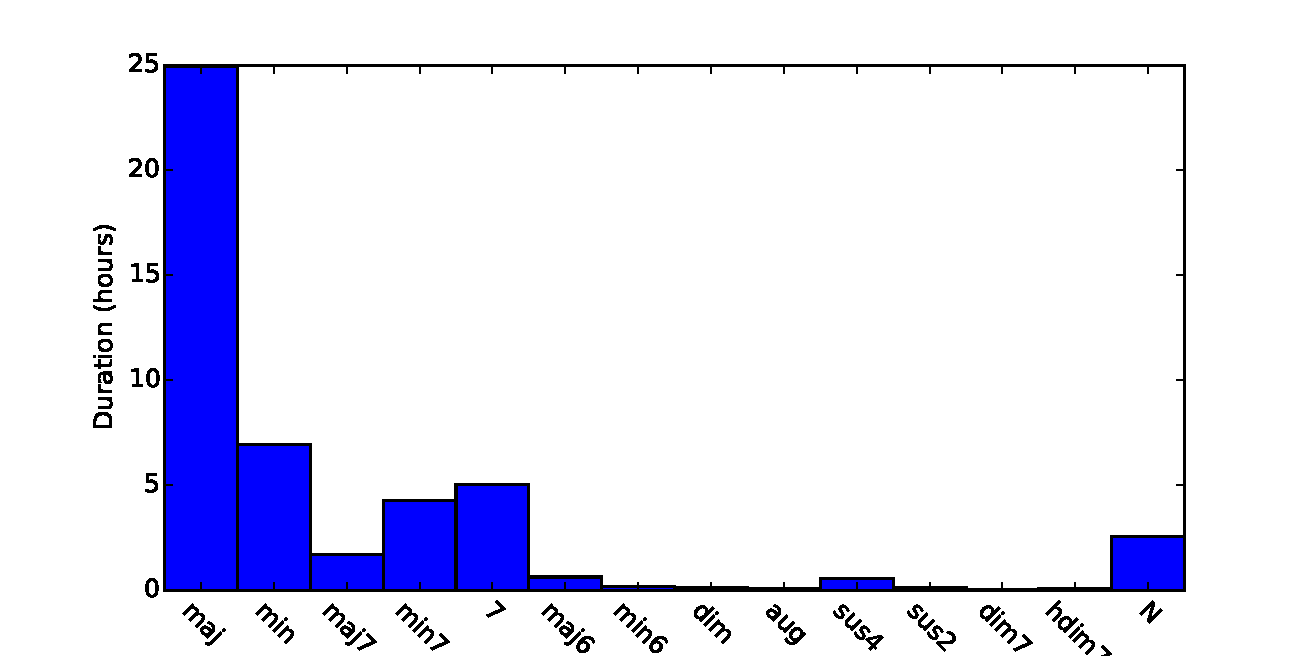
\includegraphics[width=\textwidth]{training_distribution}
\caption{Histogram of chord qualities in the merged data collection.}
\label{fig:training_distribution}
\end{figure}


\subsection{Experimental Setup}
\label{subsec:experimental_setup}
This work proceeds directly from the previous study, and takes a similar approach in many facets.
There are a handful of important distinctions to make between the two, however, and these differences are detailed here.

\subsubsection{Input Representation}
\label{subsubsec:data_considerations}
A comparable constant-Q transform is applied to the audio at a framerate of 20Hz, without subsequent low-pass filtering or decimation, and time-frequency patches are formed from 20 frames, corresponding to 1 second.
Whereas the previous study aimed to learn context directly, there is the inherent concern that a low input framerate will reduce the amount of data available for training beyond what is required by the model.
In lieu of learning this context, standard post-filtering will be applied in the form of a uniform-transition HMM with a tunable self-transition penalty, consistent with \cite{Cho2014Improved}; this is introduced in greater detail shortly, in \ref{subsubsec:viterbi}.

Additionally, local contrast normalization is included as a standard preprocessing stage, with minor modifications.
In previous work, a threshold is placed on the scaling term given by the average standard deviation over the entire input.
While this may be suitable in the field of computer vision, where spatial dimensions are equivalent in 2-space, audio data behave differently in time and frequency.
Namely, complex sounds often exhibit an overtone series, and energy becomes more densely concentrated in higher frequencies.
This can have the undesirable effect of inadequately gaining regions that are more sparse.
To correct for this behavior, the scaling coefficient is adjusted such that the frequency range considered is a piecewise function of frequency height, defined as follows:

% TODO: this is unclear.

\begin{align*}
X_{filt} = (X \circledast W) \\
V = X_{filt} - X \\
S_k = V \circledast W_k \\
S_k = max(S_k, \mu_{S_k}) \\
Y = \sum_{k=0}^{K-1} g_k * \frac{V}{S_k} \\
\end{align*}

\noindent To illustrate the benefit of this piecewise combination, an example track is given in Figure \ref{fig:lcn_mods}, both with and without the octave-dependent modification.

\begin{figure}[!t]
\centering
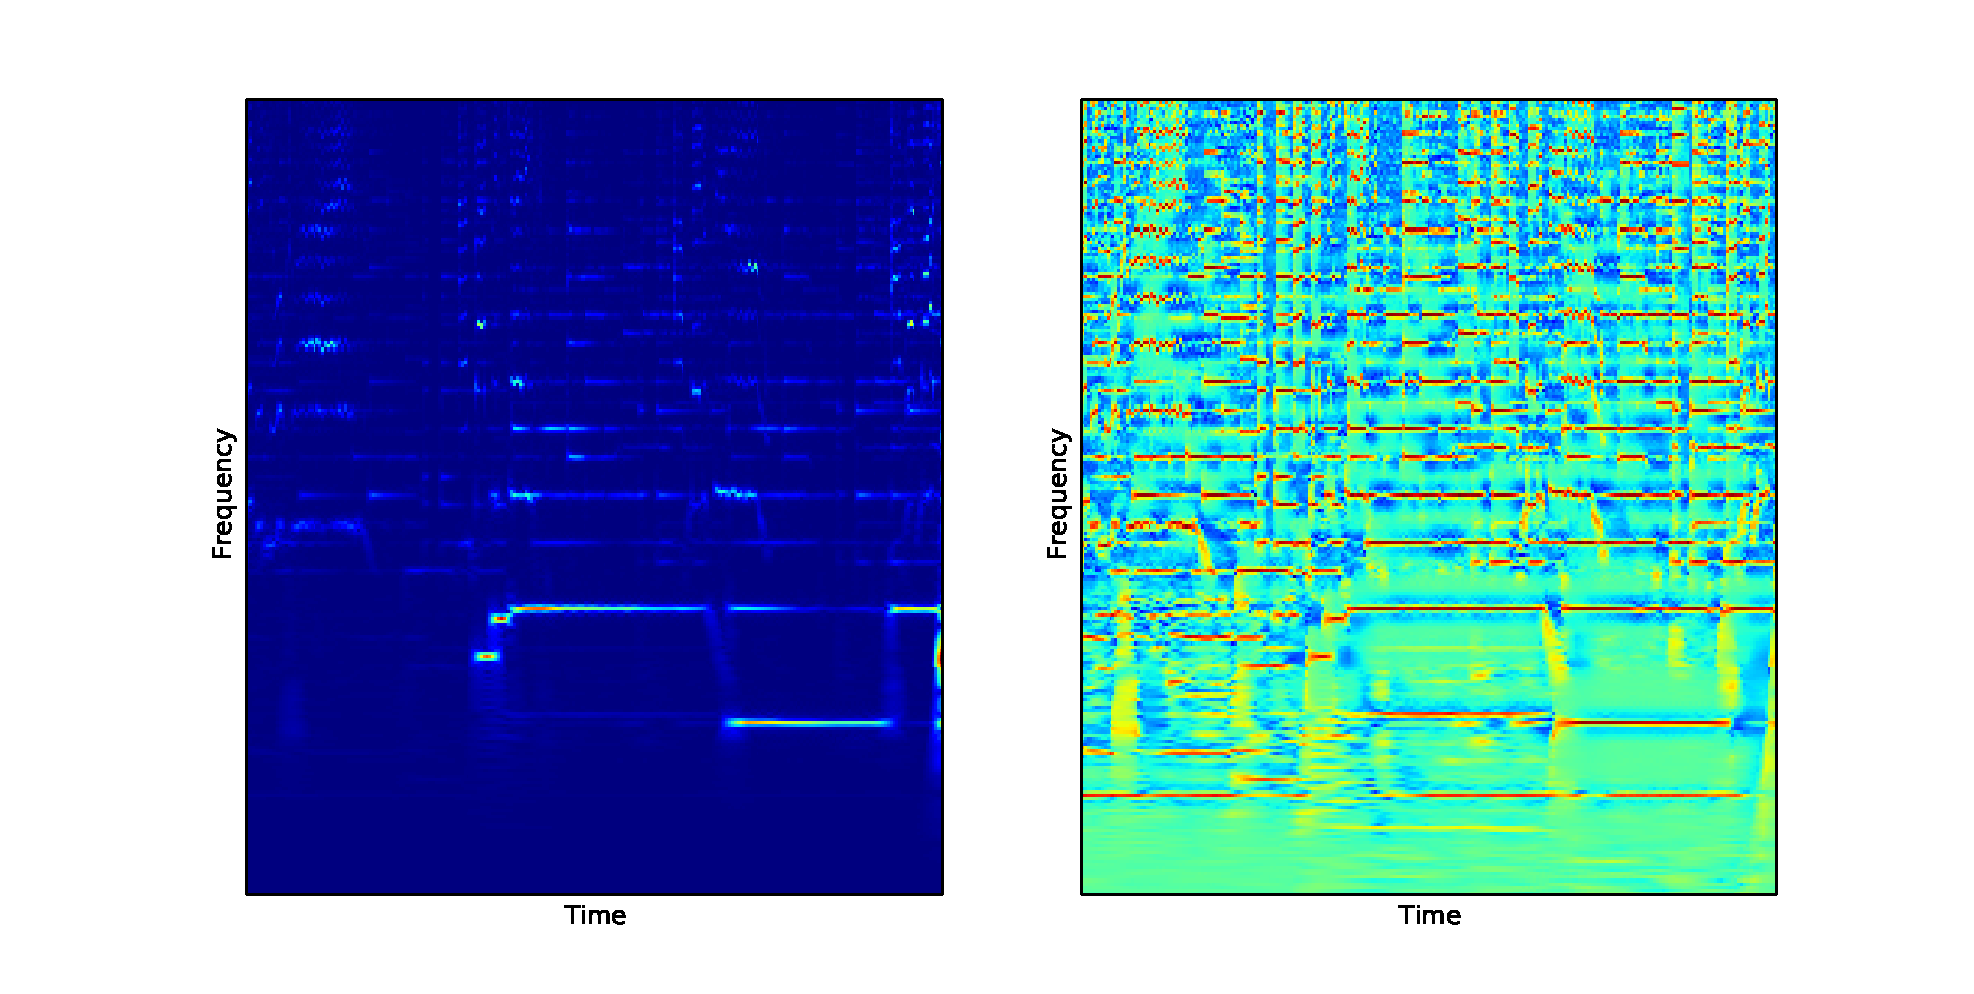
\includegraphics[width=\textwidth]{cqt_compare}
\caption{The visible effects of octave-dependent LCN, before (left) and after (right).}
\label{fig:lcn_mods}
\end{figure}


\subsubsection{Designing a Root-Invariant Classifier}
\label{subsubsec:root_invariance}
One of the key findings from the previous study of deep networks for ACE, consistent with previous research, is the importance of enforcing or encouraging root-invariance in the model.
With GMMs, this is typically achieved by rotating all data, i.e. chroma features, to the same root and fitting a model for each quality.
Then, when applying the model, likelihoods are estimated for each root by circularly rotating chroma through all twelve positions to recover the full space of chord classes.
In the pilot study on chord estimation, this concept was mimicked by rotating the data in the input domain.
While this data augmentation helped produce better results, it is a somewhat inelegant approach to realize pitch-invariance.
During training, the model must learn the same representation for all 12 pitch classes in order to represent each quality in every root.
Not only does this require more parameters to capture this redundant information, but it will likely require more training iterations for the model to do so.

Alternatively, pitch invariance can be built directly into the model by tying the weights of the classifier for different chord qualities across the twelve roots.
This is realized here by defining a four layer network composed entirely of convolution operations, diagrammed in Figure \ref{fig:fullconvnet}.
As convolutional networks amply demonstrated, weight tying is an effective way to achieve translation invariance with fewer parameters and less training data.
This is achieved as follows: the penultimate representation is designed to yield a matrix with shape $(12 \times N)$, corresponding to the number of pitch classes and the chosen output dimensionality of the second to last layer, respectively; the chord classifier is then applied by taking the inner product with a weight matrix with shape $(N \times 13)$, corresponding to the dimensionality of the previous layer and the number of chord qualities, respectively.
For ease and efficiency this is implemented as a convolution, but the result is equivalent.
This produces a $(12 \times 13)$ matrix, which is flattened to represent the 13 qualities in all possible roots.

The no-chord class is not captured by this operation, however, and a separate fully connected layer is applied in parallel to the flattened penultimate representation to estimate this class independently.
This one-dimensional no-chord estimator is then concatenated with the flattened chord estimator, and this combined representation of 157 classes is normalized by the softmax operation to yield the probability mass function over all classes.

\begin{figure}[!t]
\centering
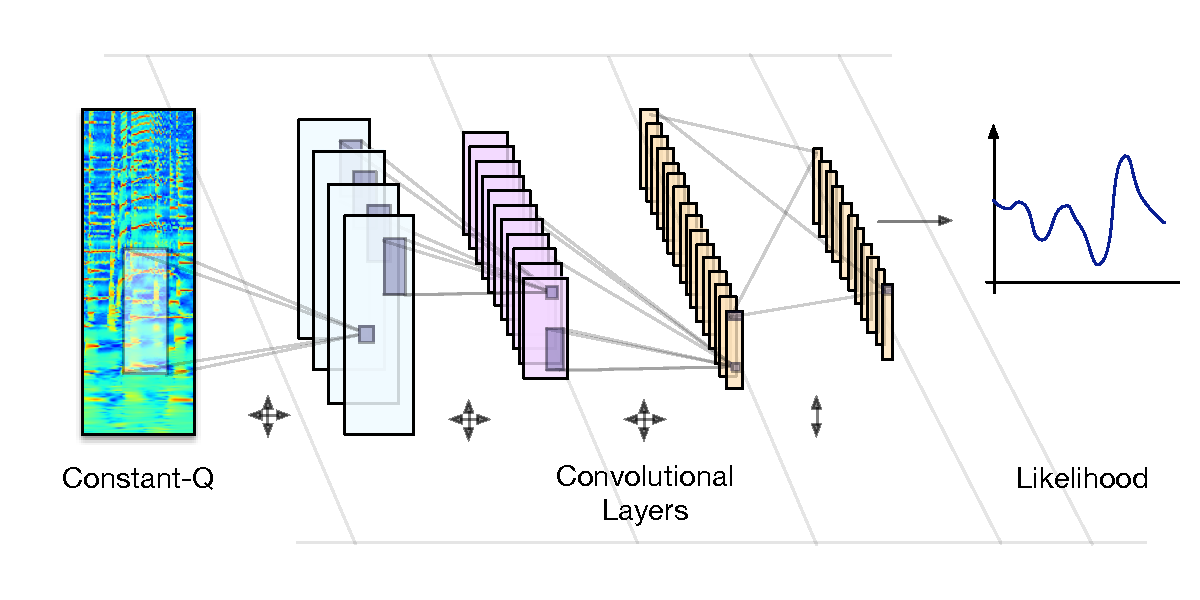
\includegraphics[width=\textwidth]{fullconvnet}
\caption{A Fully Convolutional Chord Estimation Architecture.}
\label{fig:fullconvnet}
\end{figure}

\subsubsection{Convolutional Dropout}
\label{subsubsec:conv_dropout}

Here, the principles of dropout, discussed in Chapter \ref{chp:deep_learning}, are extended to 3D convolutions.
In the weight-matrix case, training with dropout effectively ignores activations of an transformed output, setting them to zero.
Considering each output coefficient as a measure of activation for a given ``feature'', the act of dropout can be interpreted as sub-sampling the feature extractors learned by the model.

By extension, the same principle could be applied to convolutional layers.
In the absence of any known prior effort to do so, this is achieved here by dropping out a full 3D kernel.
% The former is chosen as a trade-off in the degree of randomness dropout introduces to the training processes; the merits of one approach over another are left for future work.
Expressed formally, the $i^{th}$ kernel, $W_i$, can be masked with probability $p$, resulting in the possibly empty feature map, $Z_i$:

\begin{equation}
\label{eq:conv_dropout}
Z_i = binomial(p) * h(X \circledast W_i + b_i) / (1.0 - p)
\end{equation}

\noindent where the output is also scaled by the complement of the probability.
Here, it is expected that each kernel learns a collection of feature extractors that, on average, work well together.
In the language of co-adaptation, the tensor can be seen as a ``team'' of feature detectors, and as such correlations are broken up at this mid, as opposed to global, level.

There are two small implementation details worth noting.
First, the same parameters in the model are dropped out over the entire batch, and not separately for each datapoint in the batch.
In the model averaging interpretation of dropout, this is analogous to updating one possible model at each update step, and offers interesting parallels to coordinate block descent.
Additionally, the original proposal of dropout suggests that the activations of all outputs be halved when using the full model at test time.
This is somewhat cumbersome in practice, and, as indicated in Eq. (\ref{eq:conv_dropout}), scale \emph{up} the parameters during training by the complement of the dropout ratio, allowing models in test to be agnostic of this process.


\subsubsection{Architectural Considerations}
\label{subsubsec:arch}

Given the theoretical relationship between dropout and model averaging, it is reasonable to expect that larger dropout ratios will necessitate larger architectures.
Therefore, a variety of model complexities are explored by changing the number of kernels in each layer; the primary weight shapes of the networks are given in Table \ref{tab:lvce_archs}:

\begin{table}[t]
\begin{center}
\caption{Parameter shapes in the three model complexities considered.}
\label{tab:lvce_archs}
\begin{tabular}{l | c | c | c | c }
layer & L & XL & XXL & pooling\\
\hline
0   & (16,  1, 5, 13) & (20,  1, 5, 13) & (24,  1, 5, 13) & (2, 3) \\
1   & (32, 16, 5, 37) & (40, 20, 5, 37) & (48, 24, 5, 37) & (2, 1) \\
2   & (64, 32, 1, 33) & (80, 40, 1, 33) & (96, 48, 1, 33) & (2, 1) \\
3.a & (13, 64, 1,  1) & (13, 80, 1,  1) & (13, 96, 1,  1) &   --   \\
3.b &    (768, 1)     &     (960, 1)    &    (1152, 1)    &   --   \\
\hline
\end{tabular}
\end{center}
\end{table}

The first four layers are 3D-convolutions, and thus the weights are 4 dimensional, corresponding to the number of kernels, the number of input feature maps, filter size in the time dimension, and filter size in the frequency dimension, respectively.
The first three of these layers make use of max-pooling in time by a factor of 2, but only the first also performs max-pooling in frequency, by a factor of 3.
As before, downsampling in frequency is performed in the spirit of learning slight tuning invariance, consistent with 12-TET.
The final layer, 3.b, corresponds to the fully-connected no-chord regressor, and the shape of this weight matrix is given as the input and output dimensionality, respectively.


\subsubsection{Correcting Class Imbalance with Scaled Likelihood Estimation}
\label{subsubsec:scaled_likelihood_estimation}
Having defined the output of the model as a probability function, it is straightforward to again optimize the parameters to the negative log-likelihood over the dataset.
However, there are two difficulties that prohibit the uniform presentation of classes, as in previous work.
First, due to the increased number of classes, mini-batches would either need to consist of many datapoints, increasing the processing time of each batch, or the learning rate would need to be smaller or diminishing over time to prevent oscillation, increasing the number of iterations necessary to converge.
To the latter point, it is easy to imagine scenarios where gradient descent wobbles back and forth between updates, as each batch pulls the parameters in a slightly different direction.
The other challenge this raises is a result of the considerable class imbalance, where uniform presentation would both spend too much time on minority classes and inhibit the speed at which the model could learn the full extent of the majority classes.

The solution to this problem is found in Bayes' theorem, where the network is understood as yielding a class posterior probability, $P(Y|x)$, for the chord class, $Y$, given the observation, $x$:

\begin{equation}
P(x|Y) = \frac{P(Y|x)P(x)}{P(Y)}
\end{equation}

The observation likelihood, $P(x|Y)$, is then a function of the posterior, the class prior, $P(Y)$, and probability of the observation itself, $P(x)$.
This final quantity is independent and thus can be ignored:

\begin{equation}
P(x|Y) \varpropto \frac{P(Y|x)}{P(Y)}
\end{equation}

While the deep network is trained to produce the class posterior, the class prior can be measured empirically over the training set, and divided out after the fact.
Referred to as \emph{scaled likelihood estimation}, this strategy has proven effective at reducing the effects of class imbalances in the functionally related domain of automatic speech recognition \cite{Dahl2012Context}.
Notably, scaled likelihood estimation is particularly attractive here because it scales well with the number of estimated classes.

As a final comment, a possible pitfall when applying likelihood scaling is a matter of numerical stability arising from the least represented classes, or classes that might not even occur in the training set.
Whereas this can be mitigated with pseudo-counting ---setting a heuristically determined, non-zero lower bound--- the class prior here is computed by counting each observation toward the same quality in all roots.
Though this prior could be seen as a coefficient vector to optimize in a more direct way, this approach works reasonably well in practice.


\subsubsection{Training and Early Stopping}
\label{subsubsec:early_stopping}

In contrast to the previous study, which converged to a stable result in a few thousand iterations, it takes considerably more effort to train models for this task, on the order of hundreds of thousands of iterations.
Given the lengthy run time, parameters are saved every 1k iterations during training, and frame the problem of early stopping as a brute-force search over a finite set of parameter configurations.
Due to the application of Viterbi and the coupling with the self transition penalty, validation is non-trivial and computationally expensive.
Therefore, exhaustive validation is performed every 10k iterations, starting at 5k.
The best model and self-transition penalty are chosen by finding the configuration with the highest harmonic mean over all evaluation metrics given in Section \ref{subsec:eval_methodology}.


% \subsubsection{Viterbi Post-filtering}
% \label{subsubsec:viterbi}

% Though somewhat standard at this point in ACE research, it is worthwhile to properly formalize the HMM-based post-filtering approach used here, given its considerable impact on system performance.


% \subsection{Research Questions}
% \label{subsec:research_questions}

% What can we do to overcome these issues of class imbalance?
% % Build class invariance into the model
% % use dropout during training
% % smaller inputs, more constraints, leverage HMM for context / stabilization
% How does the deep learning system compare to the state of the art?
% % Beats it! depending on who you ask, at least
% What are the advantages and challenges of training with larger vocabularies?
% % Resolve predictions back to maj / min, how does it do? Should be better...
% % Larger vocabularies result in more class collisions
% % But this is actually a manifestation of ambiguity
% Does observed system behavior correspond to quantitative evaluation?
% % Getting a lot of reasonable confusions.
% % Maybe this is a function of an inherently subjective task.
% % The ground truth data on hand were ``reviewed'', and there are no records concerning which chord names may have been contested or corrected.
% % Rock corpus


\subsection{Experimental Results}
\label{subsec:quantitative_results}


\begin{table}[t]
\scriptsize
\begin{center}
\caption{Weighted recall across metrics over the training data.}
\label{tab:recall_train}
\begin{tabular}{cc|rrrrrrr}

\hline
 \multicolumn{2}{c|}{Model} &   triads &   root &  MIREX &   tetrads &   sevenths &   thirds &   majmin \\
\hline
\hline
\multicolumn{2}{c|}{Cho, 2014} &   0.8053 & 0.8529 &  0.8205 &    0.6763 &     0.6823 &   0.8261 &   0.8109 \\
\hline
 L &  0.0 & 0.9087 & 0.9249 &  0.9140 & 0.8600 & 0.8601 &   0.9177 &   0.9097 \\
 & 0.125 &   0.8706 & 0.9018 &  0.8785 &    0.7798 &     0.7792 &   0.8895 &   0.8718 \\
 &  0.25 &   0.8382 & 0.8811 &  0.8490 &    0.7266 &     0.7277 &   0.8637 &   0.8405 \\
 & 0.5 &   0.7916 & 0.8491 &  0.8079 &    0.6577 &     0.6641 &   0.8262 &   0.7970 \\
\hline
  XL &   0.0 &   0.9236 & 0.9353 &  0.9277 &    0.8903 &     0.8906 &   0.9300 &   0.9244 \\
   &  0.125 &   0.8899 & 0.9145 &  0.8962 &    0.8217 &     0.8214 &   0.9049 &   0.8908 \\
   &  0.25 &   0.8504 & 0.8888 &  0.8610 &    0.7374 &     0.7385 &   0.8734 &   0.8527 \\
   &  0.5 &   0.7972 & 0.8541 &  0.8118 &    0.6632 &     0.6683 &   0.8329 &   0.8014 \\
\hline
  XXL &  0.0 &   0.9462 & 0.9528 & 0.9487 &    0.9297 &     0.9300 &   0.9498 &   0.9466 \\
   &   0.125 &   0.8994 & 0.9209 &  0.9048 &    0.8386 &     0.8374 &   0.9133 &   0.8997 \\
   &   0.25 &   0.8701 & 0.9041 & 0.8777 &    0.7833 &     0.7828 &   0.8921 &   0.8710 \\
   &   0.5 &   0.8043 & 0.8573 &  0.8184 &    0.6783 &     0.6820 &   0.8374 &   0.8080 \\
\hline
\end{tabular}
\end{center}
\end{table}

Following from the setup defined above, the three model complexities ---X, XL, and XXL--- are trained with four dropout values, $p_{dropout} \in \{0.0, 0.125, 0.25, 0.5\}$ across five folds of the data.
Note that when $p_{dropout} = 0.0$, this is equivalent to training a model without dropout.
Additionally, the system presented in \cite{Cho2014Improved}, referred to here simply as ``Cho'', is trained on identical partitions of the data and evaluated alongside the deep networks.
Weighted recall for the various comparison functions, averaged across folds, is given in Tables \ref{tab:recall_train} and \ref{tab:recall_test} for the training and test splits, respectively.


\begin{table}[t]
\scriptsize
\begin{center}
\caption{Weighted recall across metrics over the test (holdout) data.}
\label{tab:recall_test}
\begin{tabular}{cc|rrrrrrr}

\hline
\multicolumn{2}{c|}{Model}  & triads &   root &   MIREX &   tetrads &   sevenths &   thirds &   majmin \\
\hline
\hline
\multicolumn{2}{c|}{Cho, 2014} &   0.7970 & 0.8475 &  \textbf{0.8147} &    0.6592 &     0.6704 &   0.8197 &   0.8057 \\
\hline
L & 0.0 &   0.7939 & 0.8442 &  0.8102 &    0.6583 &     0.6725 &   0.8135 &   0.8041 \\
  & 0.125 &   0.7951 & 0.8465 &  0.8109 &    0.6516 &     0.6616 &   0.8203 &   0.8028 \\
 & 0.25 &   0.7882 & 0.8445 &  0.8039 &    0.6509 &     0.6592 &   0.8175 &   0.7950 \\
  & 0.5 &   0.7762 & 0.8372 &  0.7936 &    0.6358 &     0.6442 &   0.8115 &   0.7832 \\
\hline
 XL &   0.0 &   0.7939 & 0.8432 &  0.8098 &    0.6589 &     0.6736 &   0.8122 &   0.8042 \\
  &  0.125 &   \textbf{0.7995} & 0.8493 &  0.8145 &    \textbf{0.6673} &     \textbf{0.6788} &   0.8227 &   \textbf{0.8077} \\
  &  0.25 &   0.7950 & 0.8479 &  0.8114 &    0.6493 &     0.6580 &   0.8215 &   0.8023 \\
  &  0.5 &   0.7773 & 0.8401 &  0.7940 &    0.6351 &     0.6430 &   0.8147 &   0.7836 \\
\hline
   XXL & 0.0 &   0.7969 & 0.8463 &  0.8130 &    0.6583 &     0.6741 &   0.8136 &   0.8080 \\
   &  0.125 &   0.7993 & 0.8477 &  0.8140 &    0.6633 &     0.6745 &   0.8215 &   0.8075 \\
   &  0.25 &   0.7947 & \textbf{0.8497} &  0.8092 &    0.6592 &     0.6686 &   \textbf{0.8241} &   0.8020 \\
   &  0.5 &   0.7768 & 0.8369 &  0.7941 &    0.6392 &     0.6468 &   0.8121 &   0.7830 \\
\hline
\end{tabular}
\end{center}
\end{table}

There are several observations that may be drawn from these two tables.
First, in the absence of dropout, the deep network models considered here are able to overfit the training data.
This is an important finding in so far as making sure that the fully-convolutional architecture is not overly constrained, and indicates that the XXL model is a reasonable upper bound on complexity.
The effect of dropout on performance over the training set is significant, as it reduces overfitting consistent with increased values.

Shifting focus to performance on the test set, it is obvious that these differences in training set performance have little impact on generalization, and all models appear to be roughly equivalent.
A small amount of dropout --0.125 or 0.25-- has a slight positive effect on generalization; too much dropout, on the other hand, seems to have a negative effect on performance.
There are two possible explanations for this behavior:
one, a high degree of convolutional dropout is more destabilizing than in the fully-connected setting;
and two, these models were not finished learning, and stopped prematurely.

Overall, the best deep networks appear to be essentially equivalent to the state of the art comparison system, referred to henceforth as ``Cho''; XL-0.125 just barely eclipses Cho in every metric but ``MIREX'', while XL-0.25 is right on its heels.
The different metrics indicate that confusions at the strict level are predominantly musically related, i.e. descending in order from root, thirds, triads, sevenths, tetrads.
Interestingly, the performance gap between the ``root'' and ``triads'' scores is quite small, $\approx 5\%$, while the gap between ``root'' and ``tetrads'' is nearly $20\%$, for all models considered.
One way to interpret this result is that these systems are quite robust in the estimation of three-note chords, but struggle to match the way in which reference annotators use sevenths.


\begin{table}[t]
\begin{center}
\caption{Quality-wise recall statistics for train and test partitions, averaged over folds.}
\label{tab:qwise_macro_recall}
\begin{tabular}{l|rrrr}
\hline
 train   &    0.0 &   0.125 &   0.25 &    0.5 \\
\hline
 L       & 0.8858 &  0.8263 & 0.7403 & 0.5838 \\
 XL      & 0.9049 &  0.8569 & 0.7652 & 0.6147 \\
 XXL     & 0.9421 &  0.8838 & 0.8232 & 0.6459 \\
\hline
 test   &    0.0 &   0.125 &   0.25 &    0.5 \\
\hline
 L      & 0.4306 &  0.5029 & 0.5240 & 0.5135 \\
 XL     & 0.4174 &  0.4887 & \textbf{0.5281} & 0.5253 \\
 XXL    & 0.3935 &  0.4825 & 0.5127 & 0.5257 \\
\hline
\end{tabular}
\end{center}
\end{table}

The results for quality-wise recall are given in Table \ref{tab:qwise_macro_recall}.
While dropout is again able to considerably reduce over-fitting in the training set, it appears to have a more profound effect here towards generalization.
Whereas before a 0.5 dropout ratio seemed to result in the ``worst'' deep networks, here it leads to the best generalization across all chord qualities.
Furthermore, the best performing models, according to weighted recall, are not the best performing models in this table.
Thus these results allude to the notion that overall weighted recall may have an inverse relationship with quality-wise recall.


\begin{table}[t]
\begin{center}
\scriptsize
\caption{Individual chord quality accuracies for the XL-model over test data, averaged across all folds.}
\label{tab:ind_qwise_macro}
\begin{tabular}{l|ccccc|c}
\hline
    &   support (min) &    0.0 &   0.125 &   0.25 &    0.5 & Cho \\
\hline
 C:maj     &  397.4887 & 0.7669 &  0.7390 & 0.6776 & 0.6645 & 0.7196\\
 C:min     &  105.7641 & 0.5868 &  0.6105 & 0.6085 & 0.6001 & 0.6467\\
 C:7       &   68.1321 & 0.4315 &  0.5183 & 0.5783 & 0.5362 & 0.5959\\
 C:min7    &   63.9526 & 0.4840 &  0.5263 & 0.5954 & 0.5593 & 0.5381\\
 N         &   41.6994 & 0.7408 &  0.7679 & 0.7875 & 0.7772 & 0.5877\\
 C:maj7    &   23.3095 & 0.5802 &  0.6780 & 0.7268 & 0.7410 & 0.6587\\
 \hline
 C:sus4    &    8.3140 & 0.2380 &  0.3369 & 0.3811 & 0.4231 & 0.3894\\
 C:maj6    &    7.6729 & 0.1929 &  0.2908 & 0.3847 & 0.3540 & 0.3028\\
 C:sus2    &    2.4250 & 0.1921 &  0.3216 & 0.3698 & 0.3995 & 0.1993\\
 C:dim     &    1.8756 & 0.4167 &  0.4105 & 0.4140 & 0.3955 & 0.5150\\
 C:min6    &    1.5716 & 0.2552 &  0.3870 & 0.4505 & 0.5076 & 0.3129\\
 C:aug     &    1.2705 & 0.3730 &  0.5078 & 0.5346 & 0.5521 & 0.3752\\
 C:hdim7   &    1.1506 & 0.3840 &  0.5688 & 0.6659 & 0.6140 & 0.4593\\
 C:dim7    &    0.5650 & 0.2012 &  0.1790 & 0.2186 & 0.2296 & 0.0643\\
 \hline
 total & -- & 0.4174 &  0.4887 & 0.5281 & 0.5253 & 0.4546 \\
\hline
\end{tabular}
\end{center}
\end{table}

To further assess this claim, the individual chord quality accuracies are broken out by class for XL-0.125, and compared alongside Cho, given in Table \ref{tab:ind_qwise_macro}.
Immediately obvious is the influence of sharp distribution effects in generalization.
Performance for the majority chord qualities, in the upper half of the table, is noticeably higher than the minority classes, in the lower half.
The one exception is that of dominant 7 chords, which seems relatively low, especially compared to Cho;
this is likely a result of V vs V7 confusions, but the annotations do not easily provide this functional information to validate the hypothesis\footnote{The Billboard dataset \emph{does} provide tonic information, and thus this relationship could be recovered from the data; however, it is left here as a fertile area for future work}.
XXL-0.25 yields near identical weighted recall statistics to Cho, but achieves a significant increase in quality-wise recall, $R_{Q}$, 0.5127 to 0.4546 ($\delta$0.0581).


Notably, the only chord quality to decrease in accuracy with dropout is major, indicating that, with the addition of dropout, the decision boundary between major and its related classes, e.g. major 7 and dominant 7, shift.
However, because of the significant imbalance in the support of each quality, given here in minutes, a small drop in accuracy for major yields a considerable drop in weighted recall overall.
To illustrate, between the 0.125 and 0.25 dropout ratios, major accuracy drops 6\%, while dominant 7 and major 7 accuracy increase 6\% and 5\%, respectively.
In terms of overall time though, this comes at the expense of 24 minutes of major now being classified ``incorrectly'', compared to a combined 5 minutes of dominant and major 7's now being ``correct''.
Therefore, it seems there is a trade-off between these two measures, and thus the representational power of the model does not really change.
Rather, the decision boundaries between overlapping classes must prefer one over the other, and thus model selection may ultimately be a function of use-case.
For example, is it better to have a model that predicts simpler chords, i.e. major, most of the time? Or to have a model that makes use of a wider vocabulary of chords?
Lastly, it is necessary to recognize that, while quality-wise recall provides a glimpse into more nuanced system behavior, the severe class imbalance results in a rather volatile metric.


% Consider how the algorithms agree with each other
\begin{table}[t]
\begin{center}
\scriptsize
\caption{Weighted recall scores for the two algorithms scored against each other, and the better match of either algorithm against the reference.}
\label{tab:algo_vs_algo}

\begin{tabular}{lrrrrrrr}
\hline
         &   triads &   root &   MIREX &   tetrads &   sevenths &   thirds &   majmin \\
\hline
 XL-0.25 vs Cho &   0.7835 & 0.8406 &  0.8044 &    0.6769 &     0.7072 &   0.8148 &   0.8095 \\
 Cho vs XL-0.25 &   0.7835 & 0.8406 &  0.8044 &    0.6770 &     0.6982 &   0.8148 &   0.8035 \\
 \hline
 Ref. vs $\max$(XL-0.25 | Cho) &   0.8243 & 0.8705  &  0.8402  &   0.7037   &   0.7157  &  0.8452  &  0.8331 \\
\hline
\end{tabular}
\end{center}
\end{table}

As a final investigation of algorithm performance with this particular collection of data, having the estimations of two very different computational systems affords the opportunity to explore where they do or do not agree.
First, the two algorithms are scored against each other by using one as the reference and the other as the estimation.
Then, both algorithms are evaluated against the human reference, keeping the maximum of the two scores for each track.
This second condition is similar in concept to model averaging, and serves to further highlight differences between estimations.
The results of each given in Table \ref{tab:algo_vs_algo}.

It is interesting to consider that, despite nearly equivalent performance on the metrics reported above, the algorithms match each other about as well as either matches the reference annotations.
If the systems made same mistakes, there would be better agreement between their respective outputs.
Since this isn't the case, it is safe to conclude that the errors made by one system are sufficiently different than those of the other.
This is a particularly valuable discovery, as these systems offer two sufficiently distinct, automated perspectives and can be leveraged for further analysis.
Additionally, combining the systems' estimations shows that there are some instances where one model outperforms the other, encouraging the exploration of ensemble methods in future work.

\begin{figure}[t!]
\centering
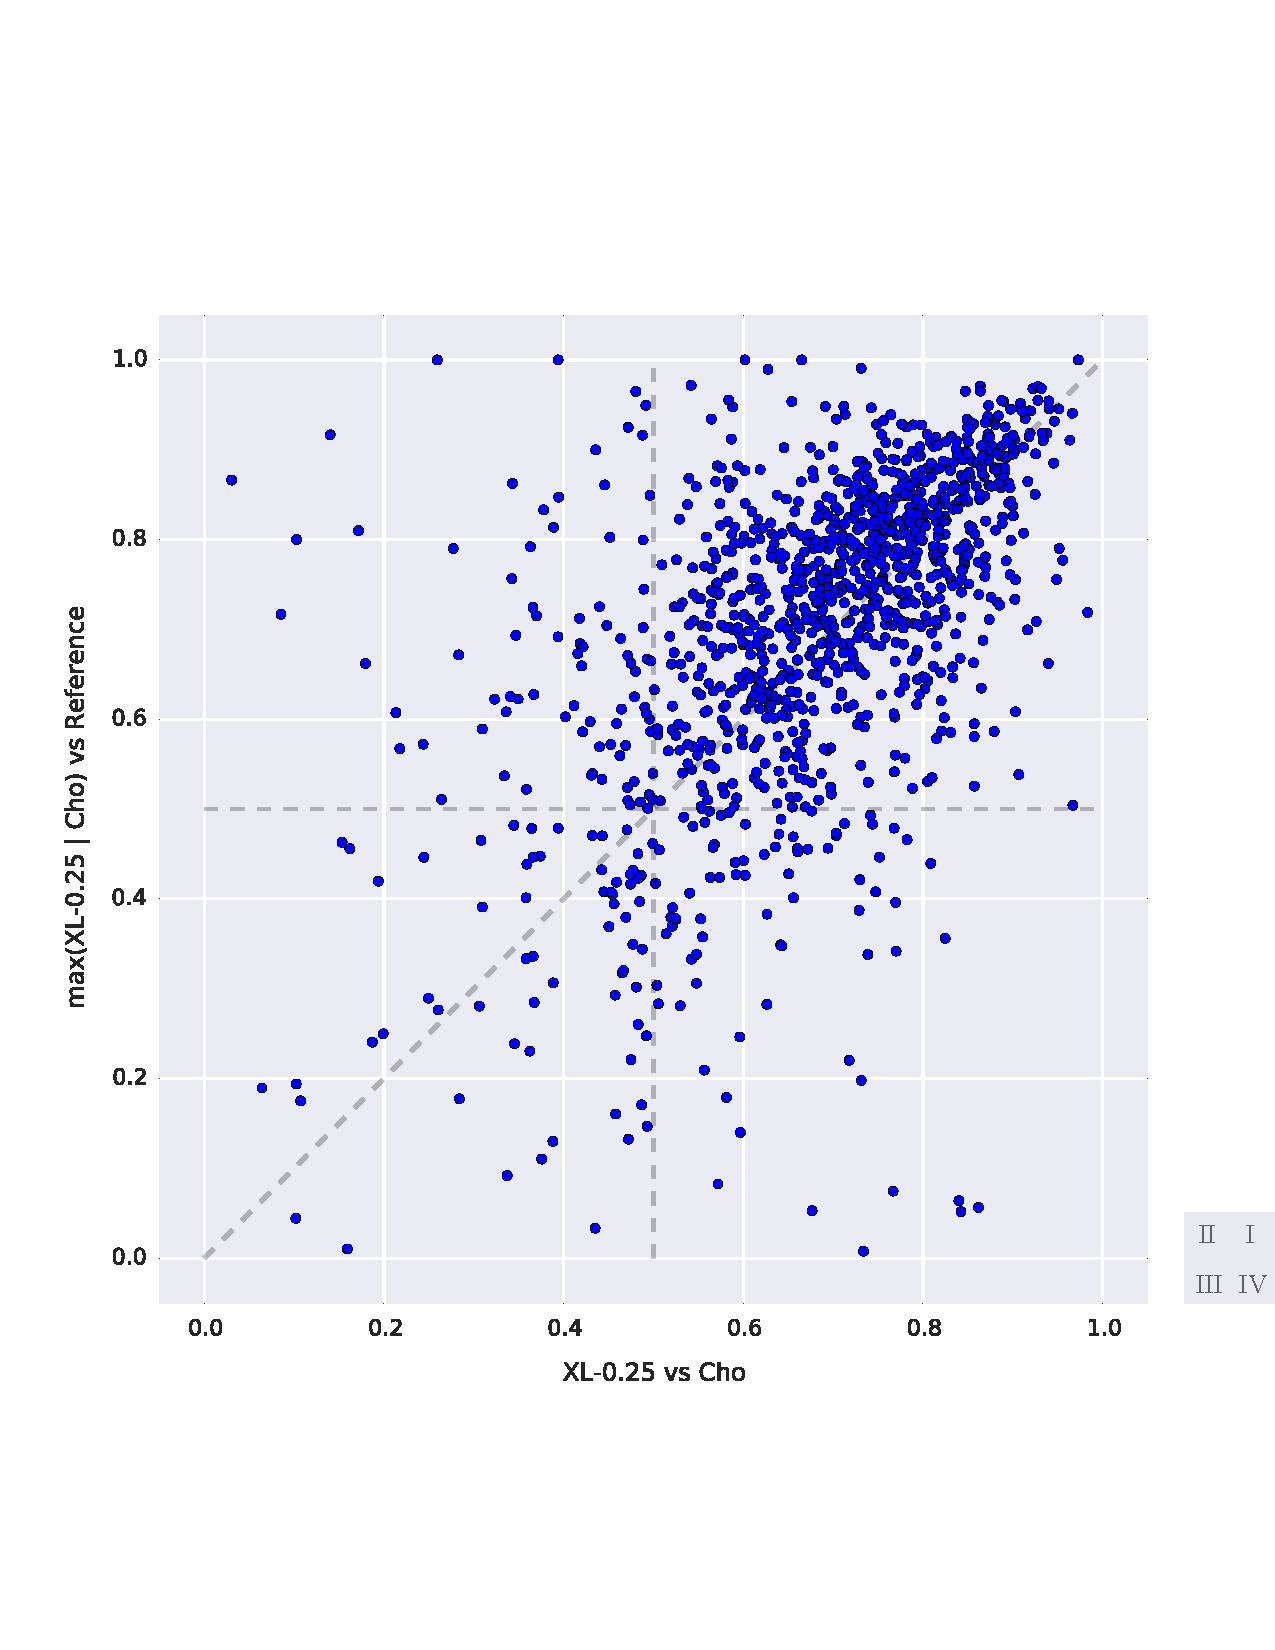
\includegraphics[width=\textwidth]{trackwise_test_agreement_annot}
\caption{Track-wise agreement between algorithms versus the best match between either algorithm and the ground truth data.}
\label{fig:trackwise_test_agreement}
\end{figure}


Expanding on this analysis, it is of considerable interest to compare scores between algorithms versus the best match with the reference on a track-wise basis; this is given in Figure \ref{fig:trackwise_test_agreement} for the ``tetrads'' metric.
Here, each track is represented as a point in coordinate space, with algorithmic agreement along the $x$-axis and best agreement with the ground truth annotations along the $y$-axis.
For clarity, this scatter plot can be understood in the following way:
the line $x=y$ corresponds to an equal level of agreement between all three chord transcriptions;
bisecting the graph horizontally and vertically yields four quadrants, enumerated I-IV in a counterclockwise manner, starting from the upper right.
Tracks that fall in each quadrant correspond to a different kind of behavior.
Points in Quadrant I indicate that both estimations and the reference have a high level of agreement ($x > 0.5$, $y > 0.5$).
Quadrant II contains tracks where the algorithms disagree significantly ($x < 0.5$), but one estimation matches the reference well ($y > 0.5$).
Tracks in Quadrant III correspond to the condition that no transcription agrees with another, ($x < 0.5$, $y < 0.5$), and are particularly curious.
Finally, Quadrant IV contains tracks where the algorithms estimate the same chords ($x > 0.5$), but the reference disagrees with them both ($y < 0.5$).


With this in mind, three-part annotations can be examined for a point in each quadrant, consisting of a reference (Ref), an estimation from the best deep neural network (XL-0.25), and an estimation from the baseline system (Cho).
In all following examples, chords are shown as color bars changing over time, from left to right;
as a convention, the pitch class of the chord's root is mapped to color hue, and the darkness is a function of chord quality, e.g. all \texttt{E:*} chords are a shade of green.
No-chords are always black, and chords that do not fit into one of the 157 chord classes are shown in gray.

\begin{figure}[t!]
\centering
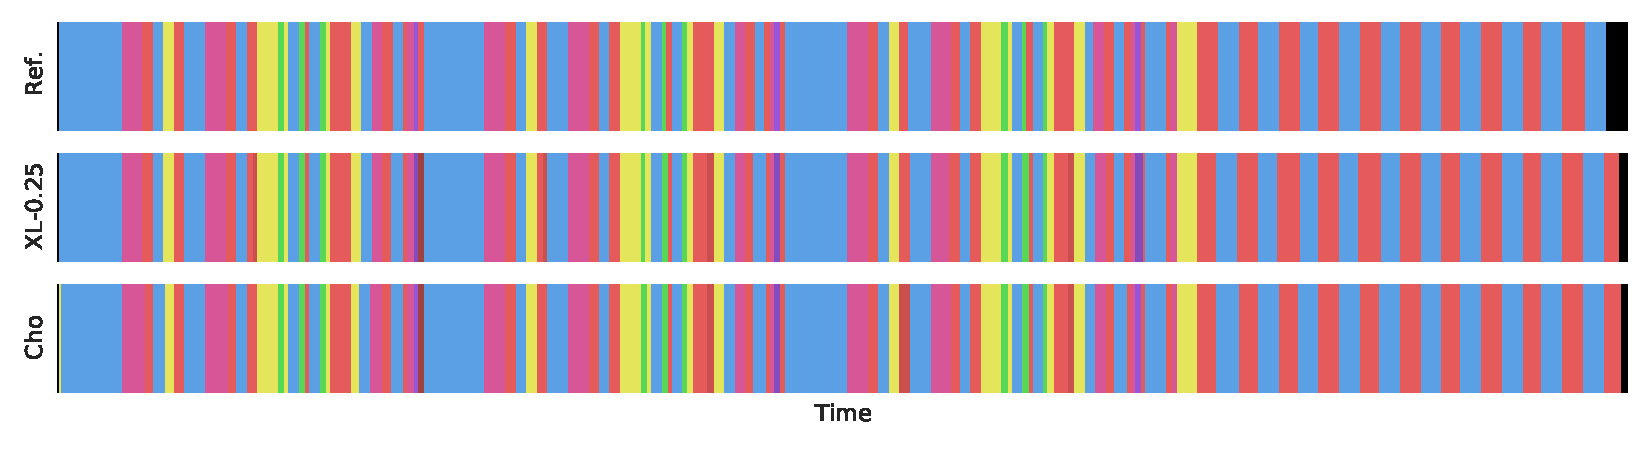
\includegraphics[width=\textwidth]{test_TRXHNQE149E2E0FFA2_annotations}
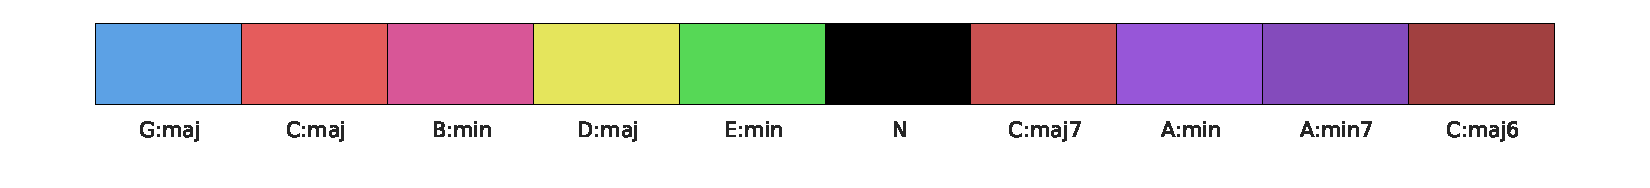
\includegraphics[width=\textwidth]{test_TRXHNQE149E2E0FFA2_legend}
\caption{Reference and estimated chord sequences for a track in Quadrant I, where both algorithms agree with the reference.}
\label{fig:test_quadI}
\end{figure}

A track from Quadrant I is given in Figure \ref{fig:test_quadI}.
As to be expected, the reference and both estimated chord sequences look quite similar.
The most notable discrepancy between the human-provided transcription and the two from the automatic methods is at the end of the sequence.
While the reference annotation claims that the transcription ends on a \texttt{G:maj}, both algorithms estimate the final chord as a \texttt{C:maj}.
This occurs because the song is in the key of G major, and thus the human chooses to end the song on the tonic chord.
However, the song ---``Against the Wind'' by Bob Seger--- is recorded with a fade-out, and the last audible part of the recording is in fact the \texttt{C:maj}, when playback volume is adjusted accordingly.
Therefore, this is an instance of the automatic systems being more precise than the human annotator.


Next, a track from Quadrant II ---``Smoking Gun'' by Robert Cray--- is considered in Figure \ref{fig:test_quadII}.
While the baseline system, Cho, agrees strongly with the reference that the predominant chord is an \texttt{E:min7}, the deep network, XL-0.25, prefers \texttt{E:min}, and produces a poor ``tetrads'' score as a result.
This confusion is an understandable one, and highlights an interesting issue in automatic chord estimation evaluation.
Depending on the instance, it could be argued that some chords are not fundamentally different classes, and thus ``confusions'' in the traditional machine learning sense, but rather a subset of a more specified chord, e.g. \texttt{E:min7} $\supset$ \texttt{E:min}.
Traditional 1-of-k classifier schemes fail to encode this nuance, whereas a hierarchical representation would better capture this relationship.

\begin{figure}[t!]
\centering
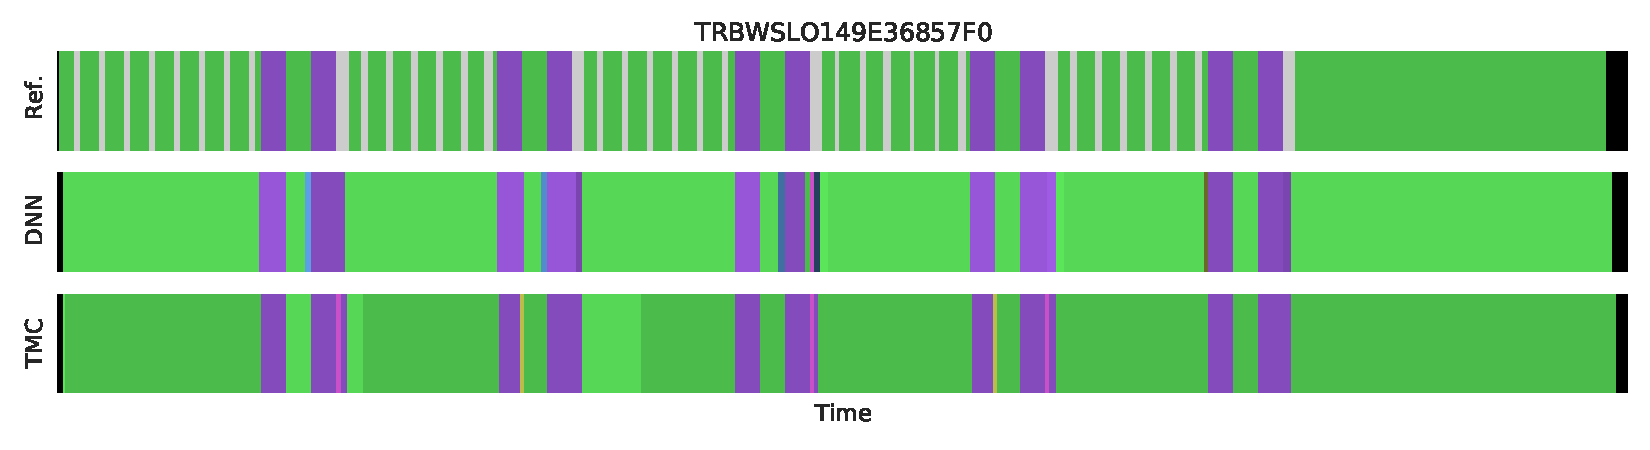
\includegraphics[width=\textwidth]{test_TRBWSLO149E36857F0_annotations}
\includegraphics[width=\textwidth]{test_TRBWSLO149E36857F0_legend}
\caption{Reference and estimated chord sequences for a track in Quadrant II, the condition where algorithms disagree sharply, but one agrees strongly with the reference.}
\label{fig:test_quadII}
\end{figure}

The track drawn from Quadrant III ---``Nowhere to Run'' by Martha Reeves and the Vandellas--- is shown in Figure \ref{fig:test_quadIII}, and especially interesting for three reasons.
First, most of the considerable disagreement between the reference and both estimated chord sequences can be explained by a tuning issue.
The automatic systems predict the tonic as \texttt{G}, while the human reference is based on \texttt{Ab}.
Matching a pure tone to this recording places the tonic around 400 Hz;
for reference to absolute pitch, the notes \texttt{G3} and \texttt{Ab3} correspond to roughly 391 Hz and 415 Hz, respectively.
Therefore, the human annotator and automatic systems disagree on how this non-standard tuning should be quantized.
Second, the two automatic systems again differ on whether to label the chord a \texttt{maj} or \texttt{7} chord;
this time, however, the reference annotation prefers the triad.
Lastly, there are three instrumental ``breaks'' in the piece where the backing band drops out to solo voice and drumset.
While the reference annotation marks the first occurrence in the song with an \texttt{X} chord label, the other two are not marked similarly despite sounding nearly identical.
The deep network model labels all three of these instances as ``no-chord,'' shown as black regions in the middle track.
This raises interesting questions regarding, among general annotator guidance, aspects of temporal continuity in a transcription.
How literal should an annotator be when marking a silence as ``no-chord''?
Is there a duration at which a gap becomes a pause?
And, of significant importance when merging various datasets, are different annotators applying the same rules and decision criteria?
% Unfortunately, none of these questions have easy answers, if any.
Taken together, this example serves to illustrate how fragile the notion of ``ground truth'' can be, due to practical issues of calibration, annotator consistency, and the instructions given during the annotation process.


\begin{figure}[t!]
\centering
\includegraphics[width=\textwidth]{test_TRVVMUA149E3780587_annotations}
\includegraphics[width=\textwidth]{test_TRVVMUA149E3780587_legend}
\caption{Reference and estimated chord sequences for a track in Quadrant III, the condition where neither algorithm agrees with the reference, nor each other.}
\label{fig:test_quadIII}
\end{figure}

\begin{figure}[t!]
\centering
\includegraphics[width=\textwidth]{test_TRNFEEU149E38D3E18_annotations}
\includegraphics[width=\textwidth]{test_TRNFEEU149E38D3E18_legend}
\caption{Reference and estimated chord sequences for a track in Quadrant IV, the condition where both algorithms agree with each other, but neither agrees with the reference.}
\label{fig:test_quadIV}
\end{figure}

As a final example from this analysis of two-part estimations, a track is considered from Quadrant IV, shown in Figure \ref{fig:test_quadIV}, corresponding to ``Some Like It Hot'' by The Power Station.
Evidenced by the large regions of estimated no-chord, both automatic systems struggle on this particular track.
Listening through, there are likely two contributing factors.
First, the song is very percussive, and heavily compressed wideband noise probably disrupts the harmonic estimates made by the models.
Second, the song makes very little use of true pitch simultaneities, and much of the harmony in this song is implied.
The song is also sparsely populated from an instrumental perspective, resulting in erroneous estimations.
While both systems appear to fall victim to this kind of content, the example speaks to the limitations of the task as it is currently defined, as well as the importance of ensuring that the content included in a dataset is relevant to the task at hand.


\subsection{Rock Corpus Analysis}
\label{subsec:qualitative_analysis}

Much can and has been said about the consistency, and thus quality, of the reference annotations used for development and evaluation of chord estimation systems.
The majority of human-provided chord annotations are often singular, either being performed by one person or as the result of a review process to resolve disagreements.
The idea of examining, rather than resolving, annotator disagreements is an interesting one, because there are two reasons why such discrepancies might occur.
The first is simply a matter of human error, resulting from typographical errors and other similar oversights.
The second, and far more interesting cause, is that there is indeed some room for interpretation in the musical content, leading to different acceptable annotations.
Most chord annotation curation efforts have made an explicit effort to resolve all discrepancies to a canonical transcription, however, and it is not possible to explore any such instances in the data used so far.



Fortunately, the \emph{Rock Corpus} dataset, first introduced in \cite{deClercq2011Corpus}, is a set of 200 popular rock tracks with time-aligned chord and melody transcriptions performed by two expert musicians:
one, a pianist, and the other, a guitarist.
This insight into musical expertise adds an interesting dimension to the inquiry when attempting to understand alternate interpretations by the annotators.
This collection of chord transcriptions has seen little use in the ACE literature, as its initial release lacked timing data for the transcriptions, and the chord names are provided in a Roman Numeral syntax.
A subsequent release fixed the former issue, however, in addition to doubling the size of the collection.
The latter issue is more a matter of convenience, as key information is provided with the transcriptions and this format can be translated to absolute chord names, consistent with the syntax in Section \ref{sec:chord_syntax}.
This dataset provides a previously uncapitalized opportunity to explore the behavior of ACE systems as a function of multiple reference transcriptions.


% What happens if the ground truth changes?

% Concurrent opinions are different from sequential opinions; this is known as ``anchoring'' and causes hysteresis in annotation.
% For example, ``Human A says X, human B doesn't disagree'' doesn't entail ``Human B says Y, human A disagrees''.

% What if either is ground truth? We can look at C(A, B) vs max(C(A, M), C(B, M)), over the rock corpus alone, to obtain many datapoints.
%

As an initial step, the two annotators, referred to here as DT and TdC, are each used as a reference and estimation perspective in order to quantify the agreement between them.
The results, given in Table \ref{tab:rc_agreement}, indicate a high, but imperfect level of consistency between the two human perspectives.
Following earlier trends, this is also a function of the chord spelling complexity, whereby equivalence at the ``root'' is much higher than for ``tetrads''.
Additionally, it is worth noting the asymmetry in chord comparisons.
Thus, depending on the perspective used as the reference, a estimation may match better or worse with it.
Finally, it is curious that the ``MIREX'' score is not perfect, a measure that focuses on pitch composition rather than contextual spelling.
One would assume that the difficulty in naming a chord is more a function of the latter than the former, but this proves not to be the case.

\begin{table}[t]
\begin{center}
\scriptsize
\caption{Weighted recall scores for the two references against each other, each as the reference against a deep network, and either against the deep network.}

\begin{tabular}{lrrrrrrr}
\hline
         &   triads &   root &   MIREX &   tetrads &   sevenths &   thirds &   majmin \\
\hline
DT vs TdC  &  0.8986 & 0.9329 &  0.9180  &   0.8355  &    0.8380  &   0.9042  &  0.9008 \\
TdC vs DT &   0.9117 & 0.9465 &  0.9168  &   0.8477  &    0.8537 &   0.9174 &    0.9176 \\
\hline
DT vs XL-0.25  &   0.7051 & 0.7816 &  0.7180  &   0.5625   &   0.5653  &  0.7314  &  0.7084 \\
TdC vs XL-0.25  & 0.7182 & 0.7939 & 0.7314  &   0.5786  &    0.5822 &   0.7444 &   0.7228 \\
\hline
$\max$(DT | TdC) vs XL-0.25 & 0.7306 & 0.8010 & 0.7431  &   0.5998  &    0.6032 &   0.7569  &  0.7348\\
\hline
\end{tabular}
\label{tab:rc_agreement}
\end{center}
\end{table}

Continuing, the deep network used in the previous analysis, XL-0.125, is again considered here.
Adopting a similar methodology as before, the estimations of the deep network are compared against both references separately, as well as against the references together and taking the better match.
Overall performance is generally worse than that observed over the holdout data in the previous investigation.
This is predominantly caused by a mismatch in the chord distributions between the datasets, as the RockCorpus only contains half the chords known to the automatic system.
Scores at the comparison of the ``root'' are much closer than that of the ``tetrads'' level, for example.
Comparing the algorithmic estimations against the intersection of the human references results in a small performance boost across all scores, indicating that the machine's ``errors'' are musically plausible, and might be validated by an additional perspective.


\begin{figure}[t!]
\centering
\includegraphics[width=\textwidth]{trackwise_rc_agreement_annot}
\caption{Track-wise agreement between annotators versus the best match between either annotator and the best performing deep network.}
\label{fig:trackwise_rc_agreement}
\end{figure}

Keeping with previous methodology, annotator agreement is compared to the better match between the estimation and either reference on a track-wise basis; this is given in Figure \ref{fig:trackwise_rc_agreement} for the ``tetrads'' metric.
Similar to Figure \ref{fig:trackwise_test_agreement}, the former is shown along the $x$-axis, and the latter along the $y$-axis.
This scatter plot can be understood similarly to before, with a few slight differences.
As before, Quadrant I contains tracks where all transcriptions agree estimation ($x > 0.5$, $y > 0.5$), and Quadrant III, where all transcriptions disagree ($x < 0.5$, $y < 0.5$).
Quadrant II now contains tracks where the \emph{annotators} disagree significantly ($x < 0.5$), but one annotator matches the reference well ($y > 0.5$), and Quadrant IV contains tracks where the annotators agree ($x > 0.5$), but the estimation disagrees with them both ($y < 0.5$).


\begin{figure}[t!]
\centering
\includegraphics[width=\textwidth]{rc_TRYCJDO14A082C24CA_annotations}
\includegraphics[width=\textwidth]{rc_TRYCJDO14A082C24CA_legend}
\caption{Reference and estimated chord sequences for a track in Quadrant I, where the algorithm agrees with both annotators.}
\label{fig:rc_quadI}
\end{figure}

Figure \ref{fig:rc_quadI} shows the three-part transcription for ``The Weight'' by The Band, a track in Quadrant I.
Again, the three chord sequences score well against each other, and offer a high degree of visual similarity.
Notably though, the algorithmic estimation independently agrees more with the interpretation of TdC than DT.
For example, there are slight discrepancies in root movement at the end of the sequence, where DT expands the \texttt{A:maj} of TdC and XL-0.25 into \texttt{A:maj}-\texttt{F\#:min}-\texttt{C\#:min}, or relatively in Roman numeral form, I-vi-iii.
This motion occurs multiple times in the song, and each annotator's interpretation is internally consistent.

\begin{figure}[t!]
\centering
\includegraphics[width=\textwidth]{rc_TRJAZCU14A0814BC9D_annotations}
\includegraphics[width=\textwidth]{rc_TRJAZCU14A0814BC9D_legend}
\caption{Reference and estimated chord sequences for a track in Quadrant II, the condition where the annotators disagree sharply, but one agrees strongly with the algorithm.}
\label{fig:rc_quadII}
\end{figure}

Being that the human annotators tend to agree more with each other than the two automatic systems previously considered, fewer tracks fall in the left half of the scatter plot in Figure \ref{fig:trackwise_rc_agreement} than Figure \ref{fig:trackwise_test_agreement}.
One of these from Quadrant II, ``All Apologies'' by Nirvana, is shown in Figure \ref{fig:rc_quadII}.
Here, the human annotators have disagreed on the harmonic spelling of the verse, with DT and TdC reporting \texttt{C\#:maj} and \texttt{C\#:7}, respectively.
On closer inspection, it would appear that both annotators are in some sense correct;
the majority of the verse is arguably \texttt{C\#:maj}, but a cello sustains the flat-$7^{th}$ of this key intermittently.
% 27 seconds in
These regions that this occurs are clearly captured in the XL-0.25 annotation, corresponding to its \texttt{C\#:7} predictions.
This proves to be an interesting discrepancy, because one annotator (DT) is using long-term structural information about the song to apply a single chord to the entire verse.

\begin{figure}[t!]
\centering
\includegraphics[width=\textwidth]{rc_TRUVQBD14A081682DB_annotations}
\includegraphics[width=\textwidth]{rc_TRUVQBD14A081682DB_legend}
\caption{Reference and estimated chord sequences for a track in Quadrant III, the condition where neither annotator agrees with the algorithm, nor each other.}
\label{fig:rc_quadIII}
\end{figure}

Another of these select few, this time from Quadrant III, is ``Papa's Got a Brand New Bag'' by James Brown, shown in Figure \ref{fig:rc_quadIII}.
In this instance, all perspectives involved disagree substantially, not only at the level of sevenths but also the quality of the third.
Exploring why this might be the case, one finds the song consists of unison riffs and syncopated rhythms with liberal use of rests.
In the absence of sustained simultaneities, most of the harmony in the song is implied, creating even more room for subjectivity on behalf of the annotators.
The automatic system, alternatively, flips back and forth between the various perspectives of the two reference annotations.
Again, the chord estimation machine has little choice but to be literal in its interpretation of solo vocal phrases, and labels such regions ``no-chord'' in the middle of the song.
This kind of repeat behavior calls attention to what is fundamentally an issue of problem formulation.
Chord \emph{transcription} is a more abstract and ultimately different task than chord \emph{recognition}, taking into consideration high-level concepts long term musical structure, repetition, segmentation or key, but conventional methodology conflates these two to some unknown degree.


\begin{figure}[t!]
\centering
\includegraphics[width=\textwidth]{rc_TRXVZFX14A0816D7D2_annotations}
\includegraphics[width=\textwidth]{rc_TRXVZFX14A0816D7D2_legend}
\caption{Reference and estimated chord sequences for a track in Quadrant IV, the condition where both annotators agree with each other, but neither agrees with the algorithm.}
\label{fig:rc_quadIV}
\end{figure}

Finally, a track from Quadrant IV ---``Every Breath You Take'' by The Police--- is given in Figure \ref{fig:rc_quadIV}.
Similar to the track considered from the same region before, the estimation is consistently a half-step flat from the references.
This pattern is indicative of a similar tuning discrepancy as before, and tuning a pure sinusoid to the track finds the tonic at approximately 426Hz, putting the song just over a quartertone flat.
Though functionally equivalent to the previous example of tuning being an issue, this instance is interesting because two annotators independently arrived at the same decision.
% Why would they both make the same mistake? Maybe it's not a mistake!
One reason this might have occurred is that, as a rock song, it makes far more sense to play in \texttt{A:maj} on guitar than \texttt{Ab:maj}.
The chord shapes involved are much easier to form in \texttt{A:maj}, and therefore more likely.
Additionally, a guitarist would probably need to change tunings to play the \texttt{Eb:maj} in the right voicing.
Taken together, it is noteworthy that such extrinsic knowledge can, and perhaps should, play a role in the process of automatic chord estimation.



\subsection{Conclusions \& Future Work}
\label{subsec:conclusions}

% Quantitative observations
Based on conventional methodology, the proposed deep learning approach leads to results on par with the state of the art, just eclipsing the baseline in the various metrics considered.
Though fully convolutional models can be complex enough to over-fit the dataset, a small amount of dropout during training helps reduce this over-fitting, while leading to slightly better generalization.
Dropout also raises quality-wise recall in minority classes significantly.
Given the significant imbalance of chord classes in the dataset, however, this is a very unstable measure of system performance.
Small shifts in the quality-wise recall of a majority class can result in large performance swings, and vice versa.
Thus, the criteria for what makes for a ``good'' system may be motivated by use case, to determine which of these metrics correspond to the desired behavior.

Additionally, the suite of chord comparison functions demonstrate that most errors between reference and estimation are hierarchical, and increase with specificity of the chord, e.g. from root to triads to tetrads.
One-of-K classifiers struggle to encode these relationships between certain chords, e.g. \texttt{A:maj} and \texttt{A:maj7}.
By analogy, this is like building a classifier that discriminates between, among other classes, animals and cats, respectively; all cats are animals, but not all animals are cats.
This is problematic in a flat classifier, because it is attempting to linearly separate a pocket of density contained within another.
To address this issue, a structured output and loss function would be better suited to model these relationships.
Directly encoding the knowledge that \texttt{maj7} chords are a subset of \texttt{maj}, will make it easier for a machine to learn these boundaries.
One such hierarchy for the chords considered in this work is given in Figure \ref{fig:chord_hierarchy}.
Here, the degree of specificity increases as the decision tree is traversed to a leaf node, and could be achieved with more structured output, such as a hierarchical softmax or conditional estimator.


\begin{figure}[t!]
\centering
\includegraphics[width=\textwidth]{chord_hierarchy}
\caption{A possible chord hierarchy for structured prediction of classes. Decisions blocks are rectangular, with the result of the previous node shown in parentheses, the semantic meaning of the node is given before a colon, and the set of valid responses is pipe-separated. Stopping conditions are given as octagons.}
\label{fig:chord_hierarchy}
\end{figure}


% On having mutliple estimators
In comparing the estimations of the two computational systems, deeper insight is gained into the ground truth data used for development, and the kinds of behavior, both the good and bad, that such approaches are prone to exhibit.
First, it is observed that they make rather different predictions and their responses could be combined, motivating the exploration of ensemble methods.
Looking at performance at the track-level, alternatively, helps identify problematic or noisy data in a collection.
This is similar in spirit to a growing body of work in MIR \cite{Zapata2012Assigning}, but it also provides some unique insight into the ACE task itself.
Computational systems tend to be precise in ways humans are not, such as continuing to predict chords during a fade-out, or reporting ``no-chord'' during a musical break.
The issue of hierarchical class relationships manifests in both models, but instances of algorithm disagreement point to music content that falls near a boundary between classes.
Such knowledge could be used to single out and review the reference chord annotation more closely.
These systems can also be sensitive to inexact tuning, and half-step deviations can be a large source of error.
Additionally, implied harmony or temporally sparse patterns can be especially problematic, resulting in an over-estimation of the ``no-chord'' class.


% On having multiple annotators
Conversely, leveraging multiple annotations for a given track provides a deeper understanding of the errors a computational system might make.
As seen here, the assessment of a system will change depending on which interpretation is taken as a reference, and a computational system may agree with another human's perspective, consistent with the work of McVicar \cite{Ni2013Understanding}.
Most important is the recognition that human annotators do not agree all the time, and that describing some music content in the language of chords is inherently subjective.
In such cases, there is no ``ground truth'' to speak of, and multiple chord labels may be acceptable.
This is a critical observation, and one that cuts strongly against the long-standing methodology of curating ground truth references in ACE.
Stated previously, the sole purpose of an objective measure is that it serves as a reasonable proxy for subjective experience.
If the goal of ACE is to produce a chord annotation on par with that of a qualified human ---a musical Turing test of sorts--- then the reference annotation at hand may be only one of many valid perspectives.
As a result, evaluating against a singular perspective is leading to results that may be inconsistent with subjective experience.

Instead, embracing multiple perspectives, rather than attempting to resolve them into a canonical target, would allow for more stable evaluation of computational models.
One such way this could be achieved is by obtaining multiple chord annotations and creating a time-aligned bag of words reference.
For example, knowing that 97 of 100 annotators labeled a chord as \texttt{A:7} is very different from the scenario that 52 did, while the other 48 reported \texttt{A:maj}.
Curating a dataset with so many perspectives is unlikely to happen, but perhaps multiple computational systems could be used to find boundary chords that \emph{do} warrant multiple perspectives.
Ultimately, this study demonstrates that future chord datasets should strive to capture the degree of subjectivity in an annotation, thus enabling objective measures better correspond with subjective experience.


\section{Summary}
\label{sec:summary}

In this chapter, the application of deep learning to ACE has been thoroughly explored.
By standard evaluation practices, competitive performance is demonstrated on both a major-minor and large-vocabulary formulation of the task.
Importantly, much effort is invested in understanding both the behavior of the computational systems discussed, as well as the reference data used to evaluate performance.
Perhaps the most important finding is that the current state of the art may have truly hit a glass ceiling, due to the conventional practice of building and testing against ``ground truth'' datasets for an all too often subjective task.
This challenge is further compounded by approaches to prediction and evaluation, which attempt to perform flat classification of a hierarchically structured chord taxonomy.
Thus, while there is almost certainly room for improvement, the exploration here indicates that the vast majority of error in modern chord recognition systems is a result of invalid assumptions baked into the very task.

Notably, four issues with current chord estimation methodology have been identified in this work.
One, it seems necessary that computational models embrace structured outputs; one-of-K class encoding schemes introduce unnecessary complexity between what are naturally hierarchical relationships.
Two, the community fundamentally needs to better distinguish between the two tasks at hand, being chord recognition ---I am playing this literal chord on guitar--- and chord transcription ---finding the best chord label to describe this harmonically homogeneous region of music--- and how this is articulated to reference annotation authors.
Three, chord transcription requires more explicit segmentation, rather than letting such boundaries between regions of harmonic stability result implicitly from post-filtering algorithms.
Lastly, the often subjective nature of chord labeling needs to be acknowledged in the process of curating reference data, and the human labeling task should combine multiple perspectives rather than attempt to yield a canonical ``expert'' reference.


% this file is called up by thesis.tex
% content in this file will be fed into the main document


\graphicspath{{6/figures/}}

\chapter{From Music Audio to Guitar Tablature}
\label{chp:background}

In the previous chapter, it was demonstrated that state of the art ACE systems perform at a relatively high level, often producing reasonable, if not exact, chord estimations.
Deploying these systems in the wild for real users, however, presents two practical difficulties:
one, performing a given chord sequence requires that the musician knows how to play each chord on their instrument of choice;
and two, the performance of classification-minded chord estimation systems does not degrade gracefully, especially for those lacking a good music theory background.
Recognizing that guitarists account for a large majority of the music community, both challenges are addressed here by designing a deep convolutional network to model the physical constraints of a guitar's fretboard, directly producing \emph{human-readable} representations of music audio, i.e. tablature.

Approaching chord estimation through the lens of guitar tablature offers a variety of critical benefits.
Guitar chord shapes impose an explicit hierarchy among notes in a chord family, such that related chords are forced to be near-neighbors in the output space.
This constrains the learning problem in musically meaningful ways, and enables the model to produce outputs beyond the lexicon of chords used for training.
The human-readable nature of the system's output is also valuable from a user perspective, being immediately useful with minimal prerequisite knowledge.
Furthermore, a softer prediction surface results in more informative errors, thus allowing for more graceful degradation of performance.
Finally, with an eye toward future work, the estimation of tablature makes it far easier for large online guitar communities to validate and, as needed, correct system outputs, regardless of skill level.

Therefore, this chapter extends a novel approach to bootstrapping the task of automatic chord estimation to develop an end-to-end system capable of representing polyphonic music audio as guitar tablature.
To encourage playability, a finite vocabulary of chord shape templates are defined, and the network is trained by minimizing the distance between its output and the best template for a given observation.
Experimental results show that the model achieves the goal of faithfully mapping audio to a fretboard representation, as well as further advancing the art in some quantitative evaluation metrics.


\section{Context}
\label{sec:context}


\begin{figure}[t!]

  \centering
  \centerline{\includegraphics[width=0.8\textwidth]{chord_tablature}}
\caption{A chord sequence (top), traditional staff notation (middle), and guitar tablature (bottom) of the same musical information, in decreasing levels of abstraction.}
\label{fig:chord_notation}
%
\end{figure}

% Rise of the guitarists
To date, the majority of research in automatic chord estimation is based on the two-fold premise that (a) it is fundamentally a classification problem, and (b) the ideal output is a time-aligned sequence of singular chord names.
That said, it is worthwhile to reconsider how the development of such systems is motivated by the goal of helping the amibitious musician learn to play a particular song.
Notably, today guitarists comprise one of the largest groups of musicans attempting to do just that.
Over the last century, the guitar, in all of its forms, has drastically risen in popularity and prevalance, both in professional and amateur settings.
Given the low start-up cost, portability, favorable learning curve, and ---courtesy of musicans like Jimi Hendrix or \emph{The Beatles}--- an undisputed ``cool factor'' in Western popular culture, it is unsurprising that guitars dwarf music instrument sales in the United States.
Based on the 2014 annual report of the National Association of Music Merchants (NAMM), a whopping 2.47M guitars were sold in 2013 in the United States, accounting for a retail value of \$1.07 \emph{billion} USD \cite{NAMM2014}; as a point of comparison, all wind instruments \emph{combined} ---the next largest instrument category--- totaled just over half that figure, at \$521M USD.

% Tablature notation
The fact that guitarists comprise such a large portion of the musician community is important, as it affects how they might prefer to interact with a chord estimation system.
While most instruments make use of traditional staff notation, fretted instruments, like lute or guitar, have a long history of using \emph{tablature} to notate music.
Illustrated in Figure \ref{fig:chord_notation}, tablature requires minimal musical knowledge to interpret, and thus offers the advantage that is easier to read, particularly for beginners.
Whereas staff notation explicitly encodes pitch information, leaving the performer to translate notes to a given instrument, tablature explicitly encodes performance instructions for a given instrument.
Though it can be difficult to accurately depict rhytmic information with tablature, this is seldom an obstacle for guitarists.
Chords-centric guitar parts typically place less emphasis on rhythm, and changes are usually aligned with lyrics or metrical position.

\begin{figure}[t!]
  \centering
  \centerline{\includegraphics[width=0.8\textwidth]{ug_compete}}
\caption{Visitor statistics for the tab website \emph{Ultimate Guitar}, as of January 2015.}
\label{fig:ug_compete}
%
\end{figure}

% Digitization and the internet
From the earliest days of personal computing, contemporary guitarists have embraced technology en masse for the creation and dissemination of ``tabs.''
Initial bandwidth and memory limitations, however, prevented the curation of high resolution images of sheet music, and symbolic representations, like MIDI, required specialized programs to render the music visually.
With small filesizes and compatibility with common text editors, ASCII ``tabs'' made it comparatively trivial to create, share, and store guitar music.
Thus, combining easy readability and a sufficient level of musical detail with technological constraints of the time period, guitar tablature spiked in popularity towards the end of the $20^{th}$ century.
As evidenced by heavily trafficked, user-curated websites like Ultimate Guitar\footnote{http://www.ultimate-guitar.com/}, modern online guitar communities continue to place a high demand on tablature.
Shown in Figure \ref{fig:compete}, this website alone sees, on average, over 2M unique visitors\footnote{Based on Compete.com analytics data, accessed on 15 March, 2015.} per month in the United States.

% Put it together
Taken together, these observations motivate an obvious conclusion.
Guitarists comprise a significant portion of the global music community, and are actively creating and using tablature as a means of learning music.
An automatic chord estimation system would be extremely valuable to this demographic, but such a system should be sensitive to the common preference for tablature.
Therefore, this chapter is an effort to steer automatic chord estimation toward a specific application, in order to address a potential use case for a very real demographic.


\section{Proposed System}

Building on previous efforts in automatic chord estiamtion, the best performing configuration presented in Chapter 5, XL-0.125, is extended here for guitar chord estimation.
As such, many design decisions remain consistent with the previous description, such as the constant-Q representation, dataset, or evaluation methodology, and are omitted from the discussion.
There are a few important differences, however, which are addressed below.
First, the architecture is modified slightly to produce fretboard-like outputs.
A strategy is then discussed for incorporating guitar chord shapes into the model.
The modified objective and decision functions are presented last, detailing how the model is optimized and use to estimate discrete chord classes.

Finally, it is worth mentioning that, despite the desire to map notes to a guitar fretboard, this approach is much closer in principle to chord estimation than automatic transcription methods.
Thus, while some previous work embraces this position in the realm of transcribing guitar recordings \cite{Barbancho2012} or arranging music for guitar \cite{Hori2013}, the only previous work in estimating guitar chords as tablature directly from polyphonic recordings is performed by the author, in \cite{Humphrey2014}.


\subsection{Designing a Fretboard Estimator}
\label{subsec:design}

So far, this study has shown deep trainable networks have proven to be a versatile, powerful, and practical approach to solving complex machine learning problems.
Thus it is a particular advantage of deep learning that various end-to-end systems can be quickly developed, provided one can express its fitness as a differentiable objective function.
This high level design strategy is exploited here by modifying the convolutional neural networks of the previous chapter to produce an output representation that behaves like the fretboard of a guitar.

For clarity, the modern guitar consists of six parallel strings, conventionally tuned to E2, A2, D2, G3, B3, and E4.
The polyphony of a guitar can be anywhere from zero to \emph{six}, the condition in which all strings are plucked, strummed, or otherwise activated.
A guitar is also fretted, such that the different pitches produced by a string are quantized in ascending order, as a result of shortening the length of the vibrating string.
A continuous pitch range may be achieved by various means, such as bending the strings, but such embellishments are rare to the point of unnecessary when addressing chords.
Thus, for the purposes here, it can be said that each string only takes a finite number of states: off (\texttt{X}), open, (\texttt{O}), or a number corresponding to the fret at which the string is held down.
As a simplification, all chords will be voiced in the first seven frets, and therefore each string can have nine mutually exclusive states.

Framed as such, the strings of a guitar can modeled as six correlated, but ultimately independent, probability mass functions.
The common approach toward achieving this behavior is by passing the output of an affine projection through a softmax function, as described in Chapter \ref{chp:method}, yielding a non-negative representation that sums to one.
Starting with the first three layers of the ``XL'' model defined previously, six independent softmax layers are used to model each string independently, and concatenated to form a 2-dimensional heatmap of the fretboard:

\begin{align*}
\label{eq:softmax_layer}
\small
Z_i = f_i(X_{l-1} \vert \theta_i) = \sigma (W_i \bullet X_{l-1} + b_i), i \in [0:6), \theta = [W_i, b_is]
\end{align*}

\noindent The activation of the $i^{th}$ string, $Z_i$, is computed by projecting the output of the penultimate layer in the network, $X_{l-1}$, against the weights, $W_i$, and added to a bias term, $b_i$.
This linear transformation is normalized by the softmax function, $\sigma$, and repeated for each of the six strings.
The overall model is diagrammed in Figure \ref{fig:guitarnet}.


\begin{figure}[t!]
  \centering
  \centerline{\includegraphics[width=\textwidth]{sys_diagram}}
\caption{Full diagram of the proposed network during training.}
\label{fig:guitarnet}
%
\end{figure}


\subsection{Guitar Chord Templates}
\label{subsec:vocabulary}

Having designed a convolutional network to estimate the active states of a fretboard, it is necessary to devise a mapping from chord transcriptions to fingerings on a guitar.
As the annotations available were curated for generic chord estimation, they  do not offer insight into how a given chord might best be voiced on a guitar.
Therefore, using the same vocabulary of 157 chords as before, a canonical chord shape ``template'' is chosen for each.
This is done in such a way so as to prefer voicings where all quality variations over a given root are maximally similar, i.e. chords of the same root are near-neighbors in fretboard space.
To illustrate, tablature representations for all templates are given in Figure \ref{fig:templates}.

It is worthwhile at this point to acknowledge the natural multiplicity of chord voicings on the guitar.
In addition to the normal variation that may occur in stacking the notes of a chord, e.g. ``open'' or ``closed'' position, there are other factors that influence the actual pitches that are played.
First, the same note can often be played in multiple positions on the fretboard.
For example, E3 can be played on the 12th fret of the first string, the 7th of the second, or the 2nd of the third.
Additionally, some standard chord voicings cannot be formed on the guitar, comfortably or otherwise.
As a result, it is common to play the 3rd degree of a chord over the octave, as the 10th, with a few exceptions resulting from open fingerings.
Perhaps most importantly, context is likely to determine how a chord is played, such that it is easier to move from one chord shape to the next.
Rather than attempt to cope with these issues now, the canonical template approach is chosen to simplify overall system design.
The choice of one template over another likely has nontrivial implications for the behavior of the model, but this is left as a variable to be explored in the future.


\subsection{Decision Functions}
\label{subsec:loss}

While estimating frets is sufficient for human interpretation, it is necessary to design two related decision functions.
First, the templates defined above must be incorporated into an objective function, such that the machine can learn to optimize this measure over the training data.
Finding inspiration in \cite{LeCun1998}, a Radial Basis Function (RBF) layer is added to the network, given as follows:

\begin{equation}
\small
\mathcal{E}(Z \vert W_T) = \sum(Z_{out} - W_{T}[k])^2
\end{equation}

\noindent where $Z$ is the output of the fretboard model, $W_T$ is a tensor of chord shape templates with shape $(K, 6, 9)$, such that $K$ is the number of chord templates, and $k$ the index of the reference class.
Note that these templates will impose the proper organization on the output of the model, and thus remain fixed during the learning process.
Since these weights are constant, minimizing this function does not require a contrastive penalty or margin term to prevent it from collapsing, i.e. making all the squared distances zero.

Additionally, in order to apply Viterbi post-filtering and fairly compare with previous results, the energy surface must be inverted into a likelihood function.
This is achieved by negating the energy function, $E$, and normalizing as a Gibbs distribution:

\begin{equation}
\small
\mathcal{L}(Y_k \vert X, \Theta) = \frac{exp(-\beta~E(Y_k \vert X, \Theta))}{\sum_i^K~exp(-\beta~E(Y_k \vert X, \Theta))}
\end{equation}

For the experiments detailed below, $\beta=1$.
It is conceivable that the choice of hyperparameter may impact system behavior when coupled with the Viterbi algorithm, but this value was empirically observed to give good results and not explored further.


\section{Experimental Method}

The focus of this chapter now shifts toward the experimental method adopted to investigate the behavior of this basic approach.
Herein, the training strategy, corresponding variables, and subsequent quantitative results are addressed in turn.

\subsection{Training Strategy}
\label{subsec:strategy}

Though it is able to incorporate musical knowledge into the architectural design, the model proposed here is unable achieve root-invariant weight sharing similarly to the one presented in the previous chapter.
This is due to root-dependent chord shapes, resulting from the nonuniform arrangement of chords on the neck of the guitar.
It is important to consider the effect this has on system performance, as well as other means of achieving ``root invariance'', and thus three different training strategies are employed here.

As a baseline condition, the model is trained with the natural distribution of the data (``as-is'').
Note that it is reasonable to expect these models to be deficient, as there may be chord class mismatch between training and test conditions, i.e. chord classes in the test partition do not occur in the training set.
To address the imbalanced learning problem, the second training condition scales the loss of each training observation by a class-dependent weight (``scaled'').
These weights are determined by computing the root-invariant prior over the training partition, taking its inverse, and standardizing the coefficients to unit mean and standard deviation.
The third and final training condition couples loss scaling with data augmentation, such that during training each datapoint is circularly shifted in frequency on the interval $[-12, 12]$ (``augmented'').
This allows the variance of each chord quality to be evenly distributed across classes, and helping prevent any missing class coverage in the training set.

Identical partitions of the dataset used in the previous chapter are employed here; the dataset is split 68:12:20, into training, validation, and test, respectively, and the partitions are rotated so that all data is used as a holdout set once.
All models are trained with mini-batch stochastic gradient descent at a batch size of 50, learning rate of 0.02, and dropout ratio of 0.125.
Training proceeded for several hundred iterations, ultimately bounded by a ceiling of 24 hours, and parameters were checkpointed every 10k iterations.
Model selection was performed as a brute force search over both the parameter checkpoints and self-transition penalty for Viterbi, from -20 to -40 in steps of 5.
The best model was chosen by the maximum of the harmonic mean of the chord evaluation metrics outlined previously.


\subsection{Quantitative Evaluation}
\label{subsec:evaluation}

In lieu of user study, earmarked here as future work, the quality of the resulting models is measured against the chord estimation task posed in Chapter 5.4.
Applying the methodology outlined above, the three training conditions were run to completion and used to predict into the space of 157 chord classes.
Given the intersection with the previous chapter, these three systems are compared to the system presented in \cite{Cho2014}, referred to as ``Cho, 2014'', and the model related to those explored here, ``XL-0.125'', referred to now as the ``root-invariant'' condition.

\begin{table}[t]
\begin{center}
\scriptsize
\caption{Micro-recall scores over the test set for two previous models, and the three conditions considered here.}
\label{tab:test_micro}
\begin{tabular}{c|rrrrrrr}

\hline
 & triads &   root &   mirex &   tetrads &   sevenths &   thirds &   majmin \\
\hline
Cho, 2014 & 0.7970 & 0.8475 & 0.8147 & 0.6592 & 0.6704 & 0.8197 & 0.8057 \\
\hline
Root-invariant (Chapter 5)  & 0.7995 & 0.8493 & 0.8145 & 0.6673 & 0.6788 & 0.8227 & 0.8077 \\
\hline
As-Is     & 0.8234 & 0.8705 & 0.8352 & 0.6855 & 0.7084 & 0.8376 & 0.8394 \\
Scaled    & 0.8156 & 0.8644 & 0.8283 & 0.6791 & 0.6994 & 0.8308 & 0.8295 \\
Augmented & \textbf{0.8294} & \textbf{0.8715} & \textbf{0.8420} & \textbf{0.6989} & \textbf{0.7167} & \textbf{0.8440} & \textbf{0.8412} \\
\hline
\end{tabular}
\end{center}
\end{table}

Overall perfomance, or ``micro-recall'', across metrics is given in Table \ref{tab:test_micro}.
It is immediately apparent from the table that the three fretboard models appear to do considerably better than either of the two previous ones.
Additionally, the combination of weight scaling and pitch shifting leads to the best overall performance.
As the second, weight scaled condition fares slightly worse than training the models with the data as-is, it is reasonable to assume that applying pitch shifting only during training likely would have resulted in higher overall scores.
However, the quality-wise, ``macro-recall'', measures, given in Table \ref{tab:test_qualitywise}, better illustrate the true impact of these strategies.

\begin{table}[t]
\begin{center}
\scriptsize
\caption{Quality-wise recall across conditions.}
\label{tab:test_qualitywise}
\begin{tabular}{c|c|ccc|c}

 quality   &  Root-invariant &  As-is & Scaled & Augmented & Support (min) \\
\hline
 maj       &  0.7390 &  0.8572 &  0.8413 &  0.8417 &  397.4887 \\
 min       &  0.6105 &  0.6516 &  0.6312 &  0.6645 &  105.7641 \\
 7         &  0.5183 &  0.2928 &  0.3001 &  0.3367 &   68.1321 \\
 min7      &  0.5263 &  0.4556 &  0.4670 &  0.5077 &   63.9526 \\
 N         &  0.7679 &  0.6670 &  0.6712 &  0.6942 &   41.6994 \\
 maj7      &  0.6780 &  0.4143 &  0.4614 &  0.5525 &   23.3095 \\
 \hline
 maj6      &  0.2908 &  0.0259 &  0.0682 &  0.1061 &    7.6729 \\
 sus4      &  0.3369 &  0.0252 &  0.0952 &  0.1747 &    8.3140 \\
 sus2      &  0.3216 &  0.0098 &  0.0146 &  0.2216 &    2.4250 \\
 aug       &  0.5078 &  0.0093 &  0.1431 &  0.3365 &    1.2705 \\
 dim       &  0.4105 &  0.2898 &  0.4030 &  0.3803 &    1.8756 \\
 min6      &  0.3870 &  0.0367 &  0.1611 &  0.3011 &    1.5716 \\
 hdim7     &  0.5688 &  0.0000 &  0.0610 &  0.3913 &    1.1506 \\
 dim7      &  0.1790 &  0.0040 &  0.0453 &  0.0391 &    0.5650 \\
 \hline
 average   &  0.4887 &  0.2671 &  0.3117 &  0.3963 &  \\
\hline
\end{tabular}
\end{center}
\end{table}

Going from the ``as-is'' to ``scaled'' conditions, the slight reduction in micro-recall is traded for an increase in averaged quality-wise recall.
This result is intuitively satisfying, as the introduction of class-dependent weights into the training process should help raise the preference for the long tail chords.
Though this can help attenuate the model's strong preference for majority chord classes, it does nothing to help address the overall deficiency of minority classes.
Therefore, when loss scaling is combined with data augmentation, the increase in performance is profound; nearly all statistics, at both the micro and quality-wise macro level, improve, some significantly.

Additionally, it can be seen that the higher overall scores in the guitar model are a result of over-predicting majority, and in particular ``major'', chords
Compared to the root-invariant model of the previous chapter, the guitar models are over 10\% better at predicting major chords alone.
Somewhat surprisingly, the root-invariant model is nearly 20\% better at dominant seven chords than any new model trained here.
This can be understood as an artifact of the intersection in fretboard space between major and dominant seven chords, coupled with the significant bias toward major chords.
Finally, as to be expected, the imbalanced distribution of chord qualities prevents the lower quality-wise scores from being reflected in the overall, micro-recall statistics.
This behavior alludes to the previous discussion regarding the apparent trade-off between global performance and quality-wise accuracy.


\begin{figure}[t!]
  \centering
  \centerline{\includegraphics[width=0.8\textwidth]{quantized}}
\caption{Understanding misclassification as quantization error, given a target (top), estimation (middle), and nearest template (bottom).}
\label{fig:quantized}
%
\end{figure}


Another important behavior to consider here is the idea that the direct estimation of a fretboard representation affords some benefit over simply projecting the predicted labels of a standard chord classifier \emph{back} onto guitar chord templates.
Typical chord estimation systems, and especially those that rely heavily on Viterbi, like \cite{Cho2014}, produce a sequence of discrete chord labels, and are thus effectively ``classifiers''.
Comparatively, fretboard estimation can be seen as regression, given the continuous output surface, but can be used for classification by identifying the closest known chord template, referred to as \emph{vector quantization}.
Thus, illustrated in Figure \ref{fig:quantized}, misclassification can be understood as a type of quantization \emph{error};
here a prediction close to, but on the wrong side of, the decision boundary is assigned to a different chord shape.
However, since the representation is human readable, it is trivial to correct the error from a \texttt{C\#:min7} to \texttt{C\#:min}.


\begin{figure}[t!]
  \centering
  \centerline{\includegraphics[width=0.8\textwidth]{quant_error}}
\caption{Cumulative distribution functions of distance are shown for correct (green) and incorrect (blue) classification, in the discrete (classification) and continuous (regression) conditions.}
\label{fig:quant_error}
%
\end{figure}

In the space of fretboard estimation, this can be quantified by comparing the distances between predictions both before and after classification, partitioned on whether or not the datapoint is correctly assigned.
First, the distances between the continuous-valued fretboard and the corresponding target template are computed and histogrammed.
Next, the estimated fretboard representations are assigned to the \emph{nearest} template, and distance is computed to the target; these distances, are also histogrammed, but only take a finite number of values.
Both probability density functions are integrated into continuous distribution functions to illustrate what ratio of the data lives within an expanding sphere, shown in Figure \ref{fig:quant_error}.
Here, it is visually apparent classification widens the gap between correct and incorrect answers.
Alternatively, in the regression scenario, nearly 20\% of these errors are closer to their correct class, accounting for well over 80\% of the data.
Importantly, the improved proximity of these errors mean that they should be easier to correct by potential users.


\section{Discussion}

Thoughts on guitar stuff.
Voronoi interpretation is interesting; could probably fudge the weights to balance the volume of a classes partition with its frequency in the dataset.
A musician might know that a the flat seventh could be moved to the octave, but this representation can encode that information directly.
Thus the system can be informative even when it's technically ``wrong'', living up to the goals of graceful degradation.

\section{Summary}

Awesometown, population you.
Shown how knowledge of the guitar can be used to constrain a deep learning system and produce human readable output.


% this file is called up by thesis.tex
% content in this file will be fed into the main document

%: ----------------------- introduction file header -----------------------
% the code below specifies where the figures are stored
\graphicspath{{7/figures/}}

\chapter{Workflows for Reproducible Research}
\label{chp:reproducibility}

In recent years, the philosophy of open source software has begun taking root in scientific research, particularly in the field of computer science.
There are several reasons why open research is beneficial to the greater body of human knowledge, but three are of particular value here.
First, sharing code and data allows others to reproduce previous results, a fundamental tenet of the scientific method.
Open source implementations are invaluable for sufficiently complex systems.
It may be near impossible to describe every minute detail in a publication necessary for someone else to replicate the obtained results;
for some works, in fact, the only artifact that can do this unambiguously is the source code itself.
Second, and in a related vein, open research makes it both easier and faster to build upon and extend the previous work of others.
Even in the instance a researcher is able to recreate a published system, the time and effort necessary to get to this point is significant and arguably unnecessary.
Granted, while there is an educational component inherent to the re-implementation of previous work, the situation is akin to long division:
it is certainly valuable to learn \emph{how} to divide by hand, but no one shuns the use of a calculator on a day to day basis.
Lastly, it is a good and responsible act to contribute tools and software back to the larger research community.
All research stands on the shoulders of previous efforts, from improving on a recently published algorithm to the decades-old linear algebra routines doing all its number crunching.
The reality is that no one individual has ever truly solved anything on their own, and sharing the fruits of one's research endeavors serves the common good.

With these motivations in mind, this chapter details the several open source contributions made in the course of this work, culminating in a single code repository used to produce the results contained herein.
These software tools consist of the following:
Section \ref{sec:jams} describes \texttt{jams}, a JSON annotated music specification and python API for rich music descriptions;
Section \ref{sec:biggie} introduces \texttt{biggie}, an HDF5 interface for interacting with notoriously big data;
Section \ref{sec:optimus} details \texttt{optimus}, a user-friendly library for building and serializing arbitrary acyclic processing graphs;
Section \ref{sec:mir_eval} discusses relevant contributions to \texttt{mir\_eval}, a transparent framework for evaluating MIR systems;
and finally, Section \ref{sec:dl4mir} outlines \texttt{dl4mir}, the framework used here to complete this research.


\section{\texttt{jams}}
\label{sec:jams}

Music annotations ---the collection of observations made by one or more agents about an acoustic music signal--- are an integral component of content-based music informatics methodology, and are necessary for designing, evaluating, and comparing computational systems.
For clarity, the scope of an annotation is constrained to time scales at or below the level of a complete song, such as semantic descriptors (tags) or time-aligned chords labels.
Traditionally, the community has relied on plain text and custom conventions to serialize this data to a file for the purposes of storage and dissemination, collectively referred to as ``lab-files.''
Despite a lack of formal standards, lab-files have been, and continue to be, the preferred file format for a variety of music description tasks, such as beat or onset estimation, chord estimation, or segmentation.

Meanwhile, the interests and requirements of the community are continually evolving, thus testing the practical limitations of lab-files.
Reflecting on this tradition, there are three unfolding research trends that are demanding more of a given annotation format:

\begin{itemize}
\item \textbf{Comprehensive annotation data}:
Rich annotations, like the Billboard dataset\cite{Burgoyne2011Expert}, require new, content-specific conventions, increasing the complexity of the software necessary to decode it and the burden on the researcher to use it; such annotations can be so complex, in fact, it becomes necessary to document how to understand and parse the format\cite{De2012Parsing}.

\item \textbf{Multiple annotations for a given task}:
The experience of music can be highly subjective, at which point the notion of ``ground truth'' becomes tenuous.
Recent work in automatic chord estimation, both here and in \cite{Ni2013Understanding}, has shown that multiple reference annotations should be embraced, as they can provide important insight into both system evaluation and the problem formulation itself.

\item \textbf{Multiple concepts for a given signal}:
Although systems are classically developed to describe observations in a single namespace, e.g. chords, there is ongoing discussion toward integrating information across various musical concepts \cite{Vincent2010Roadmap}.
This has already yielded measurable benefits for the joint estimation of chords and downbeats \cite{Papadopoulos2011Joint} or chords and segments \cite{Mauch2009Using}, where leveraging multiple information sources for the same input signal can lead to improved performance.
\end{itemize}


\noindent It has long been acknowledged that lab-files cannot be used to these ends, and various formats and technologies have been previously proposed to alleviate these issues, such as RDF \cite{Cannam2006Sonic}, HDF5 \cite{Bertin2011Million}, or XML \cite{McKay2005Ace}.
However, none of these formats have been widely embraced by the community.
Considering these options, the weak adoption of alternative formats is likely due to the combination of multiple factors.
For example, new tools can be difficult, if not impossible, to integrate into a research workflow because of compatibility issues with a preferred development platform or programming environment.
Additionally, it is a common criticism that the syntax or data model of these alternative formats is non-obvious, verbose, or otherwise confusing.
This is especially problematic when researchers must handle format conversions.
Therefore, a JSON Annotated Music Specification (JAMS) was developed to address these various needs.


\subsection{Core Design Principles}
\label{subsec:design}

In order to craft an annotation format that might serve the community into the foreseeable future, it is worthwhile to consolidate the lessons learned from both the relative success of lab-files and the challenges faced by alternative formats into a set of principles that might guide the design of a new format.
With this in mind, it is argued that usability, and thus the likelihood of adoption, is a function of three criteria:
simplicity, structure, and sustainability.

\subsubsection{Simplicity}
\label{subsubsec:simplicity}
The value of simplicity is demonstrated by lab-files in two specific ways.
First, the contents are represented in a format that is intuitive, such that the document model clearly matches the data structure and is human-readable, i.e. uses a lightweight syntax.
This is a particular criticism of RDF and XML, which can be verbose compared to plain text.
Second, lab-files are conceptually easy to incorporate into research workflows.
The choice of an alternative file format can be a significant hurdle if it is not widely supported, as is the case with RDF, or the data model of the document does not match the data model of the programming language, as with XML.

\subsubsection{Structure}
\label{subsubsec:structure}
It is important to recognize that lab-files developed as a way to serialize tabular data (i.e. arrays) in a language-independent manner.
Though lab-files excel at this particular use case, they lack the structure required to encode complex data such as hierarchies or mix different data types, such as scalars, strings, multidimensional arrays, etc.
This is a known limitation, and the community has devised a variety of ad hoc strategies to cope with it: folder trees and naming conventions, such as ``\{X\}/\{Y\}/\{Z\}.lab'', where X, Y, and Z correspond to ``artist'', ``album'', and ``title'', respectively\footnote{\url{http://www.isophonics.net/content/reference-annotations}}; parsing rules, such as ``lines beginning with `\#' are to be ignored as comments''; auxiliary websites or articles, decoupled from the annotations themselves, to provide critical information such as syntax, conventions, or methodology.
Alternative representations are able to manage more complex data via standardized markup and named entities, such as fields in the case of RDF or JSON, or IDs, attributes and tags for XML.

\subsubsection{Sustainability}
\label{subsubsec:sustainability}

Recently in MIR, a more concerted effort has been made toward sustainable research methods, which we see positively impacting annotations in two ways.
First, there is considerable value to encoding methodology and metadata directly in an annotation, as doing so makes it easier to both support and maintain the annotation while also enabling direct analyses of this additional information.
Additionally, it is unnecessary for the MIR community to develop every tool and utility ourselves; we should instead leverage well-supported technologies from larger communities when possible.

\subsection{The JAMS Schema}
\label{subsec:schema}

A JAMS object is hierarchically structured to capture all relevant information in a logically organized manner.
The primary record is an \emph{annotation}, of which a JAMS object may contain zero or more.
Annotations are comprised of \emph{observations}, which maintain a set of properties: time, duration, value, confidence, namespace.
Observations have two variants, to better handle \emph{sparse} or \emph{dense} data, such as onsets or melody, respectively.
The semantic context of an observation is specified by its \emph{namespace}, providing information about how the data in the observation should be understood.
Thus a namespace allows for easy filtering and interpretation of the data in an annotation for different music description tasks.

An annotation also maintains a \emph{metadata} object.
Annotation metadata allows for rich descriptions of \emph{who} and \emph{how} a particular record was produced.
Currently, metadata has properties such as \emph{corpus}, \emph{annotator}, \emph{validation}, \emph{curator}, to name a few fields.
Not only does this information make it easier to develop and evaluate systems with an eye to subjectivity, but it enables deeper meta-analyses of the annotations themselves.
This could be achieved by considering the observations made by annotators with different musical backgrounds or degrees of formal training, for example.

In addition to an array of annotations, JAMS objects also maintain a top-level file metadata object.
While annotation metadata sponges information about observer, file metadata tracks global information about the corresponding audio signal, with properties like \emph{title}, \emph{artist}, \emph{duration}, or \emph{identifiers}.
As there is currently no standard convention for uniquely specifying audio recordings in a global manner, file metadata exists to help link the JAMS object with the appropriate signal.

Finally, \emph{sandboxes} exist in both the top-level and annotation objects to facilitate the growth and extensibility of the format.
These are unconstrained objects that can be used as needed for anything not covered by the formal schema.
This is done in the hope that sandboxes might identify information that could be incorporated into future versions.


\subsection{Python API}
\label{subsec:jams_tools}

To facilitate the use and integration of JAMS in software projects, a Python library is publicly available and under active development\footnote{\url{http://github.com/marl/jams}}.
This application programming interface (API) provides a simple interface for reading, writing, and manipulating the information in a JAMS object.
Many common datasets are also provided in this format to further encourage adoption.
Complementing the creation and use of human annotations, JAMS makes it easier to operate on this information, such as augmenting audio and annotations in parallel\footnote{\url{http://github.com/bmcfee/muda}}.


\section{\texttt{biggie}}
\label{sec:biggie}

Common practice in machine learning frameworks, like scikit-learn\footnote{\url{http://scikit-learn.org/}}, often proceeds by massaging the training data into something like a large table, i.e. rows are individual datapoints, and columns correspond to different features, coefficients, etc.
Attempts to map this paradigm to time-varying data, such as audio, can be problematic and cumbersome in practice.
It is typically advantageous to learn on several consecutive frames of features, referred to as tiles, windows, or shingles, as was the case in all work presented here.
These tiles could be sharded from longer feature sequences into some number of discrete, equivalently shaped observations, but this is generally undesirable.
Doing so limits the flexibility of the researcher considering different tile sizes, requiring that the data be sharded again.
More difficult, this practice increases the footprint of the dataset linearly with the size of each observation.
Lastly, it is helpful to keep the entire feature sequence in tact, as it facilitates the application of any additional time-dependent processing, e.g. Viterbi decoding.

To achieve these ends, \texttt{biggie}\footnote{\url{http://github.com/ejhumphrey/biggie}} is the high-dimensional, signal-level equivalent to JAMS, built on two basic objects.
An \emph{entity} is a struct-like object designed to keep various numerical representations together, regardless of samplerate.
These objects are then freely written to and read from a \emph{stash}, a persistent, i.e. on-disk, key-value store.
Here, each entity is given a unique key, making it easy to align a dictionary of signals with a dictionary of annotations.
Leveraging the h5py\footnote{\url{http://www.h5py.org/}} library under the hood and based on HDF5\footnote{\url{http://www.hdfgroup.org/HDF5/}}, biggie scales to arbitrarily large datasets;
however, though it shares a common interface with in-memory dictionaries, the footprint of a stash scales gracefully with available computational resources by lazily loading data into memory.
Biggie also allows random access and data caching, greatly facilitating stochastic sampling for on-line learning\footnote{\url{https://github.com/bmcfee/pescador}}.
Perhaps most practically though, biggie serves as \emph{the} data interchange format between processing stages in the larger framework, eliminating the need for filename parsing or content-specific naming conventions; operations are written to consume and return stashes with data under the same keys.
While biggie helps address similar pain points as other libraries, like \texttt{pandas}\footnote{\url{http://pandas.pydata.org/}}, the HDF5 back-end is crucial for serializing a large collection numerical tensors in a simple, Pythonic manner.


\section{\texttt{optimus}}
\label{sec:optimus}

% What is the problemo
Deep learning tools have matured rapidly in the last half decade, with powerful choices across several programming languages.
Developed under the direction of Yoshua Bengio at the University of Montreal, Theano\footnote{\url{http://deeplearning.net/software/theano/}}, is the leading Python library for deep learning.
Boasting a large and growing user base, Theano offers all the pieces necessary for deep learning research, including symbolic differentiation, optimized C-implementations, and seamless integration with GPUs.
Though extremely powerful, useful, and expressive, there are two facets of the library that proved troublesome in the course of this work.
Serialization is can be tricky, especially for networks under active development.
The common approach to saving objects in Python, known as ``pickling'', is sensitive to modifications to the code, and thus something pickled previously may not be recoverable in the future.
Additionally, designing neural networks in Theano can be rather time-consuming, and is not the most user-friendly experience.
This is especially true when constructing non-standard architectures, such as guitar fretboard models or pairwise training strategies.

% How does optimus solve these problems
Optimus\footnote{\url{http://github.com/ejhumphrey/optimus}} is therefore an effort to address both of these problems in a maximally versatile and intuitive manner.
To simplify the creation, training, and application of neural networks, common building blocks are provided as natively serializable objects that can be wired together in a graphical manner.
% Nodes and math
Arbitrary acyclic, i.e. no loops, directed processing graphs can be architected from a large collection of \emph{nodes}, including inputs, functions, like ``Affine'' or ``Conv3D'', and outputs.
% Losses
While a large space of loss functions can be realized from these basic building blocks, a handful of standard \emph{losses} are provided, simplifying design further.
The topology between these parts is given by a routing table, and passed off to a \emph{graph}, which connects the dots and returns a callable function.
Furthermore, given the flexibility to define topologies in a processing graph, it is simple to explore a variety of modifications, such as layer-wise hyperparameters, tapping various intermediary representations as outputs, or ``cloning'' a processing node to create a deep copy of its parameters.

In addition to the user-facing advantages, robust serialization is achieved by expressing processing graph definitions as JSON and archives of multidimensional arrays.
This offers the additional benefit that it would be straightforward to port optimus models, as graph definitions and parameter bundles, across languages in the future.
Finally, as parameter assignments are expressed through named nodes and fields, it is trivial to not only save parameters but easily initialize them by arbitrary means, such as pre-training or using supervised learning on hand-crafted functions.


\section{\texttt{mir\_eval}}
\label{sec:mir_eval}

As addressed at the outset of this work, the conventional formulation of many music description tasks attempts to model the behavior of an expert human listener.
Framing the problem as a mapping between inputs and outputs allows for objective quantitative evaluation, thus providing common dimensions on which to compare algorithms and systems against each other.
The particular dimensions on which an algorithm is evaluated is almost by definition specific to the application, and different metrics have evolved over time to provide musically meaningful assessment.
Many such scoring functions are nontrivial to implement, however, and small details can give rise to variability in resulting metrics.
The Music Information Retrieval Evaluation eXchange (MIREX), the community's annual algorithm evaluation event, has helped provide common ground on which to compare different systems.
This implementation is seldom used outside MIREX due to a variety of practical difficulties, however, and instead, researchers often resort to reimplementing the same evaluation metrics.
Unfortunately these personal implementations are not standardized, and may differ in important details, or even contain bugs, confounding comparisons.
Therefore, the \texttt{mir\_eval} project aims to address these challenges for a variety of well-established tasks \cite{Raffel2014Eval}.


Though larger in scope, the contributions to the chord estimation evaluation are particularly relevant to this work.
Despite being one of the oldest MIREX tasks, evaluation methodology and metrics for automatic chord estimation is an ongoing topic of discussion, due to issues with vocabularies, comparison semantics, and other lexicographical challenges unique to the task~\cite{Pauwels2013Evaluating}.
One source of difficulty stems from an inherent subjectivity in ``spelling'' a chord name and the level of detail a human observer can provide in a reference annotation~\cite{Ni2013Understanding}.
As a result, a consensus has yet to be reached regarding the single best approach to comparing two sequences of chord labels, and instead are often compared over a set of rules, i.e Root, Major-Minor, and Sevenths, with or without inversions.

To efficiently compare chords, a given chord label is first separated into its
constituent parts, based on the syntax of~\cite{Harte2010Towards}.
For example, the chord label \texttt{G:maj(6)/5} is mapped to three pieces of information: the root (``G''), the root-invariant active semitones as determined by the quality shorthand (``maj'') and scale degrees (``6''), and the bass interval (``5'').
Based on this representation, an estimated chord label can be compare with a reference by defining a comparison function between these invariant representations.
Any encoded chords that are deemed to be ``out of gamut'' return a negative score to be easily filtered.
Track-wise scores are computed by weighting each comparison by the duration of its interval, over all intervals in an audio file.
This is achieved by forming the union of the boundaries in each sequence, sampling the labels, and summing the time intervals of the ``correct'' ranges.
The cumulative score, referred to as \emph{weighted chord symbol recall}, is tallied over a set audio files by discrete summation, where the importance of each score is weighted by the duration of each annotation~\cite{Mauch2010Automatic}.


\section{\texttt{dl4mir}}
\label{sec:dl4mir}

Leveraging these various software components, an aggregate framework representing all work presented herein is also made available, referred to as \texttt{dl4mir}\footnote{\url{http://github.com/ejhumphrey/dl4mir}}.
At a high level, this resource contains the additional functionality necessary to reproduce this work.
For convenience, the majority of processes can be executed via a series of shell scripts to perform feature extraction, training, and evaluation.
All reported results and figures provided in this document are survived in IPython notebooks for both reference and repeatability.
Furthermore, dependencies have been minimized to make this framework sufficiently independent.
% Goals
In addition to the immediate goal of reproducing experimental results, this is done in the hope that it may facilitate future extensions of this work.
Serialized versions of important network models are also included to make comparisons against similar work easier, or to simply build them into other systems.
Finally, the source code is provided so that it will serve as another example of how one might architect a flexible deep learning framework.


\section{Summary}
\label{sec:summary}

This chapter has covered the various libraries and programming tools developed in the course of this work:
\texttt{jams}, a JSON format and Python API for music annotation;
\texttt{biggie}, an HDF5 interface for managing large amounts of numerical data;
\texttt{optimus}, a versatile yet intuitive approach to building, training, and saving deep networks;
and \texttt{mir\_eval}, an open framework for evaluation.
Not only are many of these components independently useful to deep learning workflows, but the software necessary to repeat the research reported here is made publicly available online, in the form of \texttt{dl4mir}.
Following the spirit of reproducible research, these efforts aspire to make it easier to repeat, compare against, and extend the work presented, ultimately serving the greater music informatics community.

\graphicspath{{8/figures/}}
\chapter{Conclusion}
\label{chp:conclusion}

This thesis has explored the application of deep learning methods to the general domain of automatic music description, focusing on timbre similarity and automatic chord estimation.
Encouraging performance is obtained in both areas, advancing the state of art in the latter, while providing deeper insight to the tasks at hand.
These observations encourage the slight reformulation of chord estimation as a representation learning, rather than a classification, problem, resulting in a high performing system with myriad practical benefits.
This chapter summarizes the main contritributions of this work, and offers perspectives for the future, including an assessment of outstanding challenges and the potential impact of continued research in this domain.

\section{Summary}

Automatic music description is at the heart of content-based music informatics research.
This is necessary for problems where manual annotation does not scale, such as acoustic similarity, as well as problems where most people lack the musical expertise to perform the task well, such as transcription.
While this topic is independently valuable, it would seem that progress is decelerating, and thus any efforts to correct this course must first determine why.
In Chapter \ref{chp:context}, common practice in automatic music description was revisited, leading to the identification of three deficiencies worth addressing:
hand-crafted feature design is not sustainable, shallow architectures are fundamentally limited, and short-time analysis alone fails to capture long-term musical structure.
Deep architectures and feature learning were shown to hold promise in music analysis tasks, evidenced both conceptually and by its growing success, motivating the exploration of deep learning in automatic music description.

At this point, it was necessary to consider what is ``deep learning'', and why is this an option now?
In Chapter \ref{chp:deep_learning}, the history of the field was first re-examined, showing that after an over-hyped introduction, neural networks languished through the latter part of the 20th century.
This period of skepticism and disinterest gave technology time to catch up to the theory, and after a serious of significant research contributions, deep learning made a triumphant return to the fore of computer science, toppling longstanding benchmarks seemingly overnight.
While this has brought about a second wave of hype and interest, it also encouraging the curation of a more established theory of deep networks.
As reviewed, the modern practice of deep learning consists of a handful of modular processing blocks, strung together in differentiable functions and numerically optimized to an objective function via gradient-based methods, complemented by a growing suite of practical tricks of the trade.

Having reviewed the modern core of deep learning, this work shifted focus in Chapter \ref{chp:timbre} to explore these methods directly.
As a first inquiry, a deep convolutional network was applied to the task of timbre similarity, achieving three goals:
the model is able to learn relevant signal-level features that give rise to source identification;
the resulting output space is organized in a semantically meaningful way;
and the smoothness of the space is indicated by error analysis.
The approach presented here also offers novel extensions to previous efforts in pairwise training, achieving extremely robust representations despite a considerable reduction in dimensionality.
And perhaps most importantly, these results are obtained without the need for costly subjective pairwise ratings of content.

Whereas timbre similarity served as a relatively constrained problem, Chapter \ref{chp:chord_estimation} sought to test the limits of deep learning as applied to automatic chord estimation, a well-established music informatics challenge.
Competitive performance is achieved with a deep convolutional neural network, evaluated in both a conventional and large-vocabulary variant of the task.
Somewhat more interestingly, rigorous error analysis reveals that efforts in automatic chord estimation are converging to a glass ceiling, due in large part to the objective formulation of an often subjective experience.
The problems caused by the tenuous nature of ``ground truth'' annotations are exacerbated by efforts to treat chord estimation as a flat, rather than hierarchical, classification task.
Therefore, the singlemost critical advancement facing the topic of automatic chord estimation is a re-evaluation of the task the community is attempting to solve and the data used to do so.

Despite these difficulties, the chord estimation data is leveraged to ask a slightly different question: can a model be built to automatically predict chords as guitar tablature?
Therefore, in Chapter \ref{chp:guitar}, again using a deep convolutional architecture, global performance statistics are improved over the general chord estimation system, while offering significant practical benefits.
In addition to being a high-performing system, the fretboard estiamtions are immediately human-readable and thus attractive from a user experience perspective.
Such a representation is also advantageous from a data collection, correction, and validation standpoints, significantly reducing the degree of prerequisite skill necessary to contribute annotations.

Finally, the various open source software artifacts developed in the course of this research are introduced and detailed in Chapter \ref{chp:reproducibility}:
\texttt{jams}, the structured music annotation format designed for multiplicity of both annotator perspective and task namespace;
\texttt{biggie}, an approach to managing large collections of numerical data for training stochastic learning algorithms;
\texttt{optimus}, a user-friendly library for describing and serializing trainable processing graphs;
\texttt{mir\_eval}, a suite of evaluation tools for benchmarking music description algorithms;
and finally \texttt{dl4mir}, a common framework for the systems and results presented here.


\section{Perspectives on Future Work}
\label{sec:future}

Based on the work performed herein and observations made in the process, this section offers several perspectives on deep learning, music informatics, and the intersection between them, in the spirit of helping guide future work.


\subsection{Architectural Design in Deep Learning}

Among the most common questions currently facing the application of deep learning to any problem is that of architectural design.
``How many layers,'' one might ask, ``or how many kernels are necessary for this to work?
Should I use convolutions, or matrix products, or something else altogether?
And furthermore, if and when it does actually work, what on earth is it doing?''
Admittedly, the combination of numerical optimization and extremely versatile functions often results in systems with opaque mid-level representations, earning deep networks the reputation as ``black boxes'' and the study of them a ``dark art''.
However, while these enigmatic functions might cause understandable confusion, the design of deep architectures is not necessarily devoid of intution.

% Simply train the systems we've already got
But where to start?
The simplest way one might begin to explore deep learning for some problem of choice is to build some previously published algorithm and use gradient descent to fine-tune the hand crafted weights.
There are countless MIR systems could be reformulated in the deep learning framework, such as onset detection, instrument identification, or pitch estimation.
Most importantly, doing so eliminates the need to compare minor implementation details, like specific hyperparameters or window coefficients;
just learn it and let it all come out in the wash.
Addtionally, introducing the process of learning to classic music informatics systems makes it easier to \emph{combine} multiple systems to reap the benefits of model averaging.
The key takeaway here is the notion that good architectures already exist for some problems, and that better performance can be obtained by using numerical optimization to expand the space of parameters considered.

% Or explore new ones
Critically, these lessons and practices transcend known problems to new ones.
As demonstrated with the fretboard achitecture of Chapter \ref{chp:tabbing}, systems can be quickly constructed by appropriately constraining the behavior.
Since a guitar has six strings, and each can only be active in one place, it makes sense to model each as a probability surface.
That said, there is much more could be done here.
Perhaps transition constraints could be imposed, such that the model would prefer common chord shapes, or positional constraints, whereby nearby frets are perferred to large jumps.
In this manner, end-to-end systems can be designed and developed at a high level, and numerical optimization can be leveraged to work out the fine details.
Furthermore, while learning can discover useful features that were previously overlooked or not considered, this advantage is amplified for new challenges and applications that do not offer much guiding intuition.
For tasks like artist identification or automatic mixing, it is difficult to comprehend, much less articulate, exactly what signal attributes are informative to the task and how an implementation might robustly capture this information.

% Going beyond problems that already provide some structural intuition, an advantage of deep learning is it's substantial flexibility.

% Design is a skill to be learned.
% Various design decisions, such as model selection, data pre-processing, and carefully choosing the building blocks of the system, can impact performance on a continuum from negligible differences in overall results to whether or not training can, or will, converge to anything useful.
% Likewise, the same kind of intuition holds for adjusting the various hyperparameters ---learning rate, regularizers, sparsity penalties--- that may arise in the course of training.
% The important thing to recognize though is that these are skills to be learned.
% Using deep learning presents a design problem not altogether different from the one with which we are familiar, but the approach is overtly more abstract and conceptual, placing a greater emphasis on high-level decisions like the choice of network topology or appropriate loss function.

% Abstraction
Thus, deep learning, as an approach to system design, transforms the challenge from ``how do I \emph{implement} the desired behavior?'' to ``how do I \emph{achieve} the desired behavior?''
The nature of this advantage is illustrated by the relationship between programming in a high-level language, like Python, and a low-level one, like assembly.
Technically speaking, both can be used to the same ends, but high-level languages allow for faster development of complex systems by abstracting away the minute details, like memory management or the laborious task of moving data around registers.
% Knowledge of low-level operation is often critical to success in its higher level counterpart, but powerful languages do not absolve the developer of design.
In both cases, precise control is traded for power, leaving the developer to focus on the task at hand with greater speed and efficiency.
Note, however, that abstraction doesn't eliminate the need for sound architecture, only the need to worry about certain facets.
The fundamental design challenge is the same, but operating at a higher level of abstraction allows the deep learning researcher to build bigger systems faster.

% Takeaway: it's not really guess work, there's still work to be done.
Therefore, it is worthwhile to note that music informatics researchers are quite proficient at leveraging domain knowledge, engineering acumen, and a bit of intuition to architect signal processing systems;
how many principal components should one keep of a feature representation?
what is a suitable window size for a Fourier transform?
how many subbands should a given filterbank have?
The same intuition can and should be used to design deep networks, as discussed in the learning of chroma, the design of a tempo estimation system, or constructing instrument-specific models.
% Digital signal theory is still relevant,
Ultimately, the process of designing a deep architecture is as arbitrary or intentional as one makes it; it's only guesswork if you're guessing.


\subsection{Practical Advice for Fellow Practitioners}

%
While the previous discussion hopefully serves to address some of the mystery inherent to deep learning, it certainly entails the disclaimer of ``your mileage may vary.''
The following are a handful of guidelines accumulated in the course of research;
far more suggestion than direction, they have served well in practice.

\begin{enumerate}

\item \textbf{Data is fundamental}:
The data-driven researcher will live and die by the quality of data available.
It is widely held that lots of weakly labeled data will often trump a small amount of strongly labeled data.
The cousin of this sentiment is once you have enough data, everything will come out in the wash.
Take care to note that though this may hold for training, with caveats, the inverse is true for evaluation.
Furthermore, beware obscure biases in data.
Greedy optimization will happily yield bad solutions because of oversights in the curation of training data.
This is particularly true of regression problems.
It is possible to compensate for biased data in classification via uniform class presentation or likelihood scaling, but this can be far less obvious for continuous valued outputs.


\item \textbf{Design what you know, learn what you don't}:
As mentioned, neural networks offer the theoretical promise of the universal approximation theorem, but realizing such general behavior is far from trivial.
It is therefore crucial to leverage domain knowledge where possible.
This will typically take two forms:
one, simplify the learning problem by removing degrees of freedom known to be irrelevant to the problem;
two, constrain the learning problem to encourage musically plausible solutions.
If loudness doesn't impact one's ability to recognize chords, for example, the data should probably be normalized.
Music informatics researchers have a diverse background on which to draw, and this knowledge can be incorporated into the model or training strategy.
Notably, curriculum learning will likely become a much larger topic in the near future, and much can be incorporated from music education and pedagogy in this process.


\item \textbf{Over-fitting is your friend}:
Long heralded as the boon of deep networks, over-fitting is arguably a \emph{good} sign, and far more desirable behavior than the inverse.
Simply put, if a deep network is unable to over-fit the training data, something is likely wrong.
This is often due to one or more of the following three issues;
one, it is indicative of a problem with the data, e.g. the observations and targets are uncorrelated or, worse, conflicting;
two, the chosen model lacks the representational power to fit the training data;
or three, and most problematic, the learning problem is poorly posed and optimization is getting stuck in a bad local minima.
The methods for dealing with such issues are not so well codified, but consist of data cleaning, exploring ``bigger'' models, unsupervised pre-training, changing the loss function, etc.; that said, the efficacy of such approaches will vary case by case.


\item \textbf{Get good mileage out of greedy optimization}:
Gradient descent and other such greedy methods are certainly prone to bad local minima, but it is not impossible to take active measures to discourage unfortunate solutions.
% Encourage good behaviour and discourage the bad.
Additionally, it may be easier to define the kinds of things a model \emph{shouldn't} do than the things it should.
For example, a fretboard prediction network could incorporate a penalty whereby ``unplayable'' chord shapes incur significant loss to help keep outputs in a realistic space.


\item \textbf{The gap between ``real'' and synthetic music is closing}:
As more modern music transitions to a digital environment, the difference in quality between a real sound recording and one synthesized for research purposes is converging to zero.
Generally speaking, samplers, synthesizers, and other music production software are underutilized in data-driven music research.
These high quality tools can also be used for data augmentation to make algorithms robust to irrelevant deformations, such as perceptual codecs, background noise, tempo modulation, or pitch shifting.
By generating an unprecedented amount of realistic training data, can we functionally solve tasks such as onset detection, pitch detection, or tempo estimation?

\end{enumerate}


\subsection{Limitations, Served with a Side of Realism}

% Part of a larger arc
As some of its forebears recognize and advocate, especially those who persevered through the first AI winter, it is crucial to maintain reasonable expectations for what can be achieved with deep learning.
Shown in Figure \ref{fig:deephype}, it is interesting to consider that, to date, the path of deep learning has roughly followed Gartner's hype cycle for emerging technologies:
after a most promising start followed by a period of disinterest, neural networks have sharply returned to prominence.
% This trajectory is far from finished, however, and it is yet to be determined if the topic is ready for productivity or may fall victim to another winter.

\begin{figure}
\begin{centering}
\includegraphics[width=0.6\textwidth]{deephype}
\caption{Gartner Hype cycle, applied to the trajectory of neural networks, consisting of five phases: (a) innovation, (b) peak of inflated expectations, (c) trough of disillusionment, (d) slope of enlightenment, and (e) plateau of productivity.}
\label{fig:deephype}
\end{centering}
\end{figure}

% Deep learning is trending
It goes almost without saying that excitement and interest in deep learning is spiking across computer science, in academia and industry alike.
Research groups are forming based primarily on deep learning, it is being used to win increasing number of data science competitions, and the topic has become common fodder for popular science articles and interviews.
With all the success and attention, it is easy to get carried away in thinking that deep learning is the proverbial ``magic bullet'', that it might topple all problems in due time.

The reality, however, is far more modest.
Deep learning \emph{is} indeed several important things.
It is a powerful approach to non-linear system design.
Deep networks make fantastic models of physical phenomena, and could have profound use in the fields of acoustics, immersive audio, or amplifier modeling.
It is extremely versatile, and can be easily adapted in application-specific ways that other powerful machines, such as SVMs, cannot.
And, given significant gains in compute power, the combination of architectural flexibility and numerical optimization makes it an arguably efficient research strategy, at least more so than graduate students manually tuning parameters.

That said, there are a few important things deep learning is not.
It is by no means the best answer to every problem.
Deep learning is, in its current forms, still relatively data hungry and often computationally expensive.
Even in the case of unsupervised pre-training, sufficient volumes of realistic data may not be trivial to obtain, as in the case of accelerometers or gyroscopes.
To the latter point, any performance gains obtained with a deep network could be effectively negated by disproportionate increase in processing time.
Both of these limitations are like to become less important over time, but remain relevant today.
More conceptually, albeit somewhat contentiously, nor can the modern flavors of deep learning be called ``intelligent'';
echoing the ghost of Searle, a system may certainly \emph{behave} intelligently without truly \emph{being} so.
Despite the imagery evoked by metaphors and figurative language that pervade the field, deep learning has as much in common with humanity as a player piano, and learning is merely a means of programming in a data-driven manner.
This is not to say that deep learning can or will not lead to such breakthroughs, but care should be taken when differentiating metaphor from reality.

% Semantic gap, the limitation of audio signal processing systems whereby the information necessary to make some decision does not truly reside in the signal.
% Wiggins, offers ``the mysterious thing that is Music is an abstract and intangible cultural construct, which does not have physical existence in itself, but which is described by all three of these representational domains'', being the acoustic, the auditory, and the graphemic (notated) \cite{Wiggins2009}.



% Takeaways:
What should one make of deep learning then?
Suffice it to say that deep learning is just another tool ---a powerful tool, but a tool nonetheless--- to be included in the toolbelt of the information science practitioner.
Similar to the trajectories of other, now standard, methods, such as principal components analysis, Gaussian mixture models, or support vector machines, deep learning is settling into the final stage of its hype cycle, the point at which it becomes a means to solve a problem.
\emph{Is deep learning some magic bullet?}
Of course not.
\emph{Is it intelligent?}
Hardly.
But is it useful?
Can it accelerate the process of system design and implementation?
Can it allow the clever researcher to quickly vet ideas and develop complex, robust systems?
The answer to all of these is \emph{yes}.


\subsection{On the Apparent Rise of Glass Ceilings in Music Informatics}

One of the motivating factors of this work was to understand and potentially address the increasing prevalence of diminishing returns in various music description tasks, like chord estimation, genre classification, or mood prediction.
The main hypothesis resulting from an initial survey was the idea that common approaches to system design were inadequate, and another approach to system design, i.e. deep learning, might afford significant performance gains.
However, one of the most significant outcomes of this work is in some sense the most unexpected:
subtle deficiencies in methodology may be contributing as much or more to unsatisfactory results than the algorithms or approaches used to achieve them.

This finding reflects a small but growing trend in music informatics of critically assessing how the scientific method is applied to machine listening tasks, with meta-analyses of genre recognition \cite{Sturm20inf}, rhythmic similarity \cite{Esparza2014}, and music segmentation \cite{Neito2015}, to name a few.
Looking to the intersection of these areas, the research methodology of automatic music description consists of five basic steps:

\begin{enumerate}
\item Define the problem.
\item Collect data.
\item Build a solution.
\item Evaluate the model.
\item Iterate.
\end{enumerate}


With this method as a common underpinning, the evolution of content-based music informatics unfolds logically.
Though a young field, the majority of current research has converged to a handful of established tasks, as evidenced by those conducted at MIREX.
Labeled music data is notorious difficult to amass in large quantities, but resouces have grown steadily for those well-worn problems.
In cases where it has not, researchers are faced with one of two options:
curate the data themselves, or adapt an existing dataset to their problem.
Having developed a solution, it is necessary to benchmark a proposed algorithm against previous efforts.
However, to make such comparisons fairly, it is typically necessary to compute the same metrics over the same data, as the systems themselves are seldom made public.
Thus, most research efforts today focus almost exclusively on (3) and (5), adopting or otherwise accepting the other three.

It is critical to note, though, that these other methodological stages --- problem formulation, data curation, and evaluation--- have developed naturally over time at the community level, based not on globally optimal design but rather a combination of evolving understanding, inertia, and convenience.
At this point, it serves to return to an initial question posed by this work:
why \emph{are} music description systems yielding diminishing returns?
The findings of this work, particularly in the space of automatic chord estimation, corroborate the growing trend that perhaps the biggest problem facing content-based music informatics is one of methodology.

With this in mind, reconsider the case of automatic chord estimation.
What is the scope of the problem being addressed?
``Can an agent provide acceptable chord transcriptions?'' is a very different question from ``Can an agent reproduce \emph{these} chord transcriptions?''
Analysis of the Rock Corpus transcriptions showed that comparing the outputs of two expert musicians can achieve a ``yes'' and ``no'' respectively.
Does the data reflect these requirements?
Chord annotations consist of single perspectives from several anonymized annotators.
It is doubtful that all annotators are using the chord labels the same way.
How do we know when the problem is solved?
Does weighted chord symbol recall with different comparison rules correspond to subjective experience?
Not all substitutions are equal, as the distance in harmonic function between a \texttt{I:7} and a \texttt{I} is quite different from a \texttt{V:7} and a \texttt{V}, for example.

Understandably, it is easy to lose sight of the fact that research is not just the process of iterative system development, but the entire arc of the scientific method.
At this point in the trajectory of music informatics, it is conceivable that several well-worn tasks could use a reassessment of what constitutes methodological best practices.
This is hardly a novel realization, but one that warrants greater awareness within the music informatics community.
% Interestingly enough, it has been over half a decade since Wiggins offered that ``because music is first and foremost a psychological construct, there can be no externally defined truth, and systems which aim to encode musical similarity must, by definition, do so in a human-like way.''
It is necessary, but ultimately insufficient, to tirelessly pursue better solutions;
we must be as dilligent in our pursuit of better problems.


% --------------------------------------------------------------
%:                  BACK MATTER: appendices, refs,..
% --------------------------------------------------------------

% the back matter: appendix and references close the thesis


%: ----------------------- bibliography ------------------------

%\clearpage
\onehalfspacing
\bibliographystyle{apacite}

\renewcommand{\bibname}{Bibliography} % changes the header; default: Bibliography

\bibliography{backmatter/library} % adjust this to fit your BibTex file



%: ------ appendices----------------------------------------
%\appendix

\chapter{Brownie tootsie roll lollipop cookie}
\label{adx:a}

\doublespacing

Oat cake pudding sweet lemon drops gummies cookie. 
Dragee lollipop ice cream apple pie sweet roll brownie. 
Lollipop marshmallow jelly beans marzipan sugar plum chupa chups caramels toffee. 
Croissant icing chocolate cake oat cake muffin powder tart. 
Croissant wafer dessert pudding cupcake croissant. 
Cheesecake wafer sugar plum danish. 
Liquorice powder sesame snaps.


%: --------------------------- index ---------------------------

%\clearpage
% \begin{footnotesize}
% \cleardoublepage % ensure the right page
% \phantomsection % sets an anchor
% \printindex
% \end{footnotesize}



\end{document}
